\documentclass[12pt,a4paper]{report}
\usepackage[utf8]{inputenc}
\usepackage[french]{babel}
\usepackage[T1]{fontenc}
\usepackage{geometry}
\usepackage{graphicx}
\graphicspath{{screens/}{compilation/}}
\usepackage{hyperref}
\usepackage{listings}
\usepackage{xcolor}
\usepackage{float}
\usepackage{amsmath}
\usepackage{enumitem}
\usepackage{titlesec}
\usepackage{fancyhdr}
\usepackage{booktabs}
\usepackage{array}
\usepackage{longtable}
\usepackage{setspace}
\usepackage{indentfirst}
\usepackage{csquotes}
\usepackage{caption}

% Configuration de la page - Marges 2,5 cm de tous les côtés
\geometry{left=2.5cm,right=2.5cm,top=2.5cm,bottom=2.5cm}

% Configuration de la police - Times New Roman, taille 12pt
\usepackage{times}
\renewcommand{\familydefault}{\rmdefault}

% Configuration des paragraphes
% Interligne 1,5
\onehalfspacing
% Alignement justifié, alinéa 1,25 cm, espacement après 6 pts
\setlength{\parindent}{1.25cm}
\setlength{\parskip}{6pt}
\setlength{\parfillskip}{0pt plus 1fil}

% Configuration des citations - retrait et italique
\renewenvironment{quote}
  {\list{}{\rightmargin\leftmargin\leftmargin=2cm}%
   \itshape\small}
  {\endlist}

% Configuration de l'entête et pied de page
\pagestyle{fancy}
\fancyhf{}
% Entête : chapitre courant en petits caractères italiques (taille 8)
\fancyhead[C]{\fontsize{8}{10}\selectfont\itshape\leftmark}
% Pied de page : numéro de page centré sous la forme "- 5 -"
\fancyfoot[C]{- \thepage\ -}
\renewcommand{\headrulewidth}{0pt}
\renewcommand{\footrulewidth}{0pt}

% Configuration des couleurs pour le code
\definecolor{codegreen}{rgb}{0,0.6,0}
\definecolor{codegray}{rgb}{0.5,0.5,0.5}
\definecolor{codepurple}{rgb}{0.58,0,0.82}
\definecolor{backcolour}{rgb}{0.95,0.95,0.92}

% Configuration de listings pour le code SQL
\lstdefinestyle{sqlstyle}{
    backgroundcolor=\color{backcolour},
    commentstyle=\color{codegreen},
    keywordstyle=\color{magenta},
    numberstyle=\tiny\color{codegray},
    stringstyle=\color{codepurple},
    basicstyle=\ttfamily\footnotesize,
    breakatwhitespace=false,
    breaklines=true,
    captionpos=b,
    keepspaces=true,
    numbers=left,
    numbersep=5pt,
    showspaces=false,
    showstringspaces=false,
    showtabs=false,
    tabsize=2,
    language=SQL
}

\lstset{style=sqlstyle}

% Configuration de listings pour le code PHP
\lstdefinestyle{phpstyle}{
    backgroundcolor=\color{backcolour},
    commentstyle=\color{codegreen},
    keywordstyle=\color{blue},
    numberstyle=\tiny\color{codegray},
    stringstyle=\color{codepurple},
    basicstyle=\ttfamily\footnotesize,
    breakatwhitespace=false,
    breaklines=true,
    captionpos=b,
    keepspaces=true,
    numbers=left,
    numbersep=5pt,
    showspaces=false,
    showstringspaces=false,
    showtabs=false,
    tabsize=2,
    language=PHP
}

% Configuration des numérotations des tableaux et figures selon les normes
% Tableau 1. : ... et Figure 1. : ...
\renewcommand{\figurename}{Figure}
\renewcommand{\tablename}{Tableau}
\captionsetup[figure]{labelformat=simple, labelsep=period}
\captionsetup[table]{labelformat=simple, labelsep=period}

% Configuration des titres - Numérotation "Chapitre 1", "Chapitre 2", etc.
\renewcommand{\chaptername}{Chapitre}
\titleformat{\chapter}[display]
{\normalfont\huge\bfseries}{\chaptername\ \thechapter}{20pt}{\Huge}
\titlespacing*{\chapter}{0pt}{50pt}{40pt}

% Configuration de la numérotation des sections selon les normes
% I., I.1., I.1.1., 1), ✓
\setcounter{secnumdepth}{3}
\renewcommand{\thesection}{\Roman{section}.}
\renewcommand{\thesubsection}{\thesection\arabic{subsection}.}
\renewcommand{\thesubsubsection}{\thesubsection\arabic{subsubsection}.}

% Configuration des listes selon les normes
% Pour les listes numérotées : 1), 2), etc.
\renewcommand{\labelenumi}{\arabic{enumi})}
\renewcommand{\labelenumii}{\arabic{enumii})}
% Pour les listes à puces : ✓
\renewcommand{\labelitemi}{$\checkmark$}
\renewcommand{\labelitemii}{$\checkmark$}

% Métadonnées
\title{
    \vspace{2cm}
    \Huge\textbf{rapport complet de projet de 4 modules }\\
    \vspace{1cm}
    \Large Système de Gestion de Cabinet Dentaire\\
    \vspace{0.5cm}
    \large Analyse des Besoins, Conception UML, Modèle de Données, Réalisation Logicielle, Module de Compilation, Architecture du Projet 
    \vspace{2cm}
}

\author{
    \large Projet 4 Module\\
    \vspace{0.5cm}
    \normalsize Développement d'Application Web
}
\date{\today}

\begin{document}

% Page de titre personnalisée
\begin{titlepage}
\thispagestyle{empty}
\centering

% Logo EMSI
\begin{figure}[h]
    \centering
    
\includegraphics[width=0.4\textwidth]{emsi/emsi_logo.png}
\end{figure}

\vspace{1cm}

% Titre du projet
{\Huge\textbf{PROJET}}\\
\vspace{0.5cm}
{\Large\textbf{3IIR}}\\
\vspace{1cm}
{\Large\textbf{Conception et réalisation d'un système de suivi}}\\
{\Large\textbf{des patients pour un cabinet dentaire}}\\
\vspace{0.5cm}
{\large\textbf{Ingénierie Informatique et Réseaux}}\\

\vspace{2cm}

% Encadrants à gauche et Étudiants à droite
\begin{minipage}{0.45\textwidth}
    \raggedright
    {\large\textbf{Encadrants :}}\\
    \vspace{0.3cm}
    \begin{tabular}{l}
        \large Pr. Safsouf Yassine \\
        \large Pr. Hazman Chaimae \\
        \large Pr. Ait Rai Khaoula \\
        \large Pr. El Gourari Abelali \\
    \end{tabular}
\end{minipage}
\hfill
\begin{minipage}{0.45\textwidth}
    \raggedleft
    {\large\textbf{Étudiants :}}\\
    \vspace{0.3cm}
    \begin{tabular}{l}
        \large Laknifli Khalil \\
        \large Ait Elmoumen Aymane \\
        \large Asli Oubaydoullah \\
        \large El Fellah Adil \\
        \large Ourhanim Ibrahim \\
    \end{tabular}
\end{minipage}

\vspace{2cm}

% Date
{\large\textbf{Année académique : \today}}

\end{titlepage}
\newpage

% Numérotation en chiffres romains pour les pages avant l'Introduction
\pagenumbering{roman}

% Remerciements
\chapter*{Remerciements}
\thispagestyle{empty}
\addcontentsline{toc}{chapter}{Remerciements}
\vspace*{\fill}

Nous tenons à exprimer notre profonde gratitude à tous ceux qui ont contribué à la réalisation de ce projet.

Nos remerciements vont tout d'abord à nos enseignants et encadrants pédagogiques qui nous ont guidés et apporté leur expertise tout au long de ce travail. Leur disponibilité et leurs conseils précieux ont été déterminants pour la réussite de ce projet.

Nous remercions également l'équipe pédagogique du module de Développement d'Application Web pour la qualité de l'enseignement dispensé et pour les outils mis à notre disposition.

Enfin, nous adressons nos remerciements à notre famille et à nos proches pour leur soutien indéfectible, leur patience et leurs encouragements constants durant cette période d'études.

\vspace*{\fill}
\newpage

% Résumé en Français et mots clés
\chapter*{Résumé}
\thispagestyle{empty}
\addcontentsline{toc}{chapter}{Résumé}

Ce rapport présente l'analyse complète, la conception et la réalisation d'un système de gestion de cabinet dentaire, couvrant l'ensemble du cycle de développement logiciel depuis l'analyse des besoins jusqu'à l'implémentation technique.

Le document débute par une analyse fonctionnelle et non fonctionnelle approfondie, identifiant quatre acteurs principaux (Patient, Docteur, Personnel Administratif, Système de Notifications) et leurs interactions avec le système. La modélisation UML est réalisée à travers trois diagrammes essentiels : un diagramme de cas d'utilisation avec relations \texttt{includes} et \texttt{extends}, un diagramme de séquence illustrant les interactions temporelles lors de la gestion des rendez-vous et traitements, et un diagramme de classes présentant une hiérarchie d'héritage et des relations d'association détaillées.

La conception de la base de données repose sur un schéma relationnel normalisé (3NF) implémenté sous MySQL, comprenant 11 tables principales, 3 vues optimisées pour les requêtes fréquentes, des index stratégiques et des contraintes d'intégrité référentielle complètes. Le système gère les patients, les rendez-vous avec détection de conflits, les traitements médicaux avec prescriptions, le personnel avec horaires de travail, ainsi qu'un système complet de notifications et rappels automatiques.

La réalisation logicielle présente une architecture découplée moderne : un frontend développé avec React 18, TypeScript et Tailwind CSS comprenant plus de 15 composants réutilisables et des services API organisés, et un backend Laravel 12 exposant une API RESTful complète avec 8 contrôleurs et 8 modèles Eloquent. L'authentification sécurisée utilise JWT (JSON Web Tokens) avec gestion fine des permissions selon les rôles. Le système inclut également un tableau de bord avec statistiques en temps réel, un calendrier interactif pour la gestion des rendez-vous, et une gestion complète des dossiers médicaux.

Une partie importante du rapport est dédiée au module d'analyse et de compilation, présentant une étude approfondie de cinq fonctions critiques du système. Pour chaque fonction, les cinq phases principales de compilation sont détaillées : analyse lexicale (tokenisation), analyse syntaxique (construction de l'AST), analyse sémantique (vérification de cohérence), optimisation (amélioration des performances) et génération de code. Cette analyse illustre les mécanismes internes des langages de programmation et permet d'identifier les optimisations possibles dans le code.

Le rapport se conclut par un bilan technique détaillé, présentant les compétences acquises en architecture découplée, développement frontend et backend moderne, sécurité et bonnes pratiques, ainsi que les perspectives d'évolution du système vers des fonctionnalités avancées comme la télémédecine, l'intelligence artificielle ou l'architecture microservices.

\vspace{0.5cm}
\textbf{Mots clés :} Système de gestion, Cabinet dentaire, UML, Base de données relationnelle, React, Laravel, POO, Compilation, Analyse lexicale, Analyse syntaxique, Analyse sémantique, Génération de code, Optimisation de code, Architecture, Interface

\newpage

% Abstract in English and keywords
\chapter*{Abstract}
\thispagestyle{empty}
\addcontentsline{toc}{chapter}{Abstract}

\textbf{Abstract :}

This report presents the complete analysis, design, and implementation of a dental clinic management system, covering the entire software development lifecycle from requirements analysis to technical implementation.

The document begins with an in-depth functional and non-functional analysis, identifying four main actors (Patient, Doctor, Administrative Staff, Notification System) and their interactions with the system. UML modeling is carried out through three essential diagrams: a use case diagram with \texttt{includes} and \texttt{extends} relationships, a sequence diagram illustrating temporal interactions during appointment and treatment management, and a class diagram presenting an inheritance hierarchy and detailed association relationships.

The database design is based on a normalized relational schema (3NF) implemented in MySQL, comprising 11 main tables, 3 optimized views for frequent queries, strategic indexes, and complete referential integrity constraints. The system manages patients, appointments with conflict detection, medical treatments with prescriptions, staff with work schedules, as well as a complete notification and automatic reminder system.

The software implementation presents a modern decoupled architecture: a frontend developed with React 18, TypeScript, and Tailwind CSS comprising over 15 reusable components and organized API services, and a Laravel 12 backend exposing a complete RESTful API with 8 controllers and 8 Eloquent models. Secure authentication uses JWT (JSON Web Tokens) with fine-grained permission management according to roles. The system also includes a dashboard with real-time statistics, an interactive calendar for appointment management, and complete medical record management.

A significant part of the report is dedicated to the analysis and compilation module, presenting an in-depth study of five critical system functions. For each function, the five main compilation phases are detailed: lexical analysis (tokenization), syntactic analysis (AST construction), semantic analysis (consistency verification), optimization (performance improvement), and code generation. This analysis illustrates the internal mechanisms of programming languages and enables identification of possible code optimizations.

The report concludes with a detailed technical assessment, presenting skills acquired in decoupled architecture, modern frontend and backend development, security and best practices, as well as system evolution perspectives toward advanced features such as telemedicine, artificial intelligence, or microservices architecture.

\vspace{0.5cm}
\textbf{Keywords :} Management system, Dental clinic, UML, Relational database, React, Laravel, OOP, Compilation, Lexical analysis, Syntactic analysis, Semantic analysis, Code generation, Code optimization, Architecture, Interface

\newpage

% Table des matières
\tableofcontents
\newpage

% Liste des abréviations (optionnelle - à compléter)
\chapter*{Liste des Abréviations}
\thispagestyle{empty}
\addcontentsline{toc}{chapter}{Liste des Abréviations}

\begin{description}
\item[UML] Unified Modeling Language
\item[PFA] Projet de Fin d'Année
\item[API] Application Programming Interface
\item[SQL] Structured Query Language
\item[3NF] Troisième Forme Normale
\item[JWT] JSON Web Token
\item[SPA] Single Page Application
\item[REST] Representational State Transfer
\item[ORM] Object-Relational Mapping
\item[MVC] Model View Controller
\item[CSS] Cascading Style Sheets
\item[UI/UX] User Interface / User Experience
\end{description}

\newpage

% Liste des figures
\listoffigures
\newpage

% Liste des tableaux
\listoftables
\newpage


% Passage à la numérotation en chiffres arabes à partir de l'Introduction
\pagenumbering{arabic}
\setcounter{page}{1}

% Introduction générale
\chapter{Introduction Générale}
\section{Contexte du Projet}

Ce projet consiste en l'analyse et la conception d'un système complet de gestion de cabinet dentaire. Le système doit permettre de gérer les patients, les rendez-vous, les traitements, le personnel et les notifications pour différents types d'utilisateurs : patients, docteurs et personnel administratif.

Ce document présente l'analyse des besoins, la modélisation UML du système et la conception de la base de données relationnelle.

\section{Objectifs du Projet}

Les objectifs principaux de ce projet sont :

\begin{itemize}
    \item Analyser les besoins fonctionnels et non fonctionnels du système
    \item Identifier les acteurs et leurs interactions avec le système
    \item Modéliser le système à l'aide de diagrammes UML (cas d'utilisation, séquence, classes)
    \item Concevoir une base de données relationnelle normalisée et optimisée
    \item Définir les relations entre les entités du système
\end{itemize}

\section{Structure du Document}

Ce rapport est organisé comme suit :

\begin{itemize}
    \item \textbf{Chapitre 2} : Analyse des besoins et des acteurs (analyse fonctionnelle et non fonctionnelle, contraintes)
    \item \textbf{Chapitre 3} : Conception UML (diagrammes de cas d'utilisation, séquence et classes avec relations détaillées)
    \item \textbf{Chapitre 4} : Modèle de données et base de données (schéma complet, tables, relations, vues, optimisations)
    \item \textbf{Chapitre 5} : Réalisation du Projet (stack technique détaillée, architecture, API REST, composants React, fonctionnalités, interfaces, sécurité, tests)
    \item \textbf{Chapitre 6} : Module Analyse et Compilation (étude approfondie de 5 fonctions avec analyse lexicale, syntaxique, sémantique, optimisation et génération)
    \item \textbf{Chapitre 7} : Conclusion Générale (résumé, bilan technique, apports, perspectives d'évolution)
\end{itemize}

% Analyse
\chapter{Analyse des Besoins}

\section{Analyse Fonctionnelle}

\subsection{Acteurs du Système}

Le système identifie quatre acteurs principaux :

\subsubsection{Patient}

Le patient est l'utilisateur principal qui bénéficie des services du cabinet dentaire. Il peut :
\begin{itemize}
    \item Créer un compte et s'authentifier
    \item Consulter son dossier médical
    \item Prendre, modifier et annuler des rendez-vous
    \item Modifier ses informations personnelles
    \item Recevoir des notifications et rappels
\end{itemize}

\subsubsection{Docteur}

Le docteur est le professionnel médical qui fournit les soins. Il peut :
\begin{itemize}
    \item Consulter le tableau de bord avec les statistiques
    \item Voir tous les rendez-vous des patients
    \item Consulter les dossiers médicaux des patients
    \item Ajouter et modifier des traitements
    \item Consulter le planning des rendez-vous
    \item Recevoir des notifications
\end{itemize}

\subsubsection{Personnel Administratif}

Le personnel administratif gère les aspects administratifs du cabinet. Il peut :
\begin{itemize}
    \item Gérer les patients (création, modification, consultation)
    \item Gérer les rendez-vous (planification, modification, annulation)
    \item Recevoir des notifications sur les actions des patients
    \item Gérer les rappels pour les patients
\end{itemize}

\subsubsection{Système de Notifications}

Le système de notifications est un acteur externe qui gère l'envoi automatique de :
\begin{itemize}
    \item Confirmations de rendez-vous
    \item Rappels automatiques (24h avant le rendez-vous)
    \item Notifications au personnel administratif
\end{itemize}

\subsection{Fonctionnalités Principales}

\subsubsection{Gestion des Comptes et Authentification}

\begin{itemize}
    \item Création de compte pour les patients
    \item Authentification sécurisée pour tous les utilisateurs
    \item Gestion des rôles et permissions
    \item Déconnexion
\end{itemize}

\subsubsection{Gestion des Rendez-vous}

\begin{itemize}
    \item Prise de rendez-vous en ligne par les patients
    \item Vérification de la disponibilité des créneaux
    \item Modification de rendez-vous existants
    \item Annulation de rendez-vous
    \item Consultation du planning par les docteurs
    \item Gestion des rendez-vous par le personnel administratif
\end{itemize}

\subsubsection{Gestion des Dossiers Médicaux}

\begin{itemize}
    \item Consultation du dossier médical par le patient
    \item Consultation et modification du dossier par le docteur
    \item Gestion des antécédents médicaux
    \item Gestion des allergies
    \item Historique des traitements
\end{itemize}

\subsubsection{Gestion des Traitements}

\begin{itemize}
    \item Ajout de traitements par le docteur
    \item Modification des traitements
    \item Association des traitements aux dossiers médicaux
    \item Gestion des prescriptions
    \item Génération de factures
\end{itemize}

\subsubsection{Système de Notifications}

\begin{itemize}
    \item Envoi automatique de confirmations de rendez-vous
    \item Rappels automatiques 24h avant les rendez-vous
    \item Notifications au personnel lors d'actions importantes
    \item Notifications aux patients pour les rappels
\end{itemize}

\section{Analyse Non Fonctionnelle}

\subsection{Exigences de Performance}

\begin{itemize}
    \item Temps de réponse acceptable pour les opérations courantes (< 2 secondes)
    \item Support de plusieurs utilisateurs simultanés
    \item Gestion efficace des requêtes de base de données
\end{itemize}

\subsection{Exigences de Sécurité}

\begin{itemize}
    \item Authentification sécurisée des utilisateurs
    \item Gestion des rôles et permissions
    \item Protection des données médicales sensibles
    \item Chiffrement des mots de passe
\end{itemize}

\subsection{Exigences de Disponibilité}

\begin{itemize}
    \item Système disponible pendant les heures d'ouverture du cabinet
    \item Sauvegarde régulière des données
    \item Récupération en cas de panne
\end{itemize}

\section{Contraintes}

\begin{itemize}
    \item Respect de la confidentialité des données médicales
    \item Conformité aux réglementations sur la protection des données
    \item Interface intuitive pour tous les types d'utilisateurs
    \item Compatibilité avec les navigateurs web modernes
\end{itemize}

% Conception UML
\chapter{Conception UML}

\section{Diagrammes de Conception}

Le projet inclut trois diagrammes UML essentiels qui modélisent l'architecture et le comportement du système. Ces diagrammes sont essentiels pour comprendre la structure du système et les interactions entre ses différents composants.

\subsection{Diagramme de Cas d'Utilisation}

Le diagramme de cas d'utilisation présente les fonctionnalités du système du point de vue des différents acteurs. Il identifie les interactions entre les utilisateurs (acteurs) et le système.

\begin{figure}[H]
    \centering
    \includegraphics[width=0.95\textwidth]{casUtilisation.jpg} % Replace with actual UML if found
    \caption{Diagramme de cas d'utilisation du système de gestion de cabinet dentaire}
    \label{fig:use-case}
\end{figure}

\subsubsection{Acteurs Identifiés}

Le diagramme illustre les acteurs suivants :
\begin{itemize}
    \item \textbf{Patient} : Utilisateur principal qui peut créer un compte, prendre des rendez-vous, consulter son dossier médical, et recevoir des notifications
    \item \textbf{Docteur} : Professionnel médical qui peut consulter les dossiers patients, gérer les traitements, et consulter le tableau de bord
    \item \textbf{Personnel Administratif} : Personnel qui gère les patients et les rendez-vous, et reçoit des notifications
    \item \textbf{Système de Notifications} : Système externe responsable de l'envoi des notifications
\end{itemize}

\subsubsection{Cas d'Utilisation Principaux}

Les cas d'utilisation principaux incluent :

\textbf{Pour le Patient :}
\begin{itemize}
    \item Créer un compte / S'authentifier
    \item Consulter son dossier médical
    \item Prendre un rendez-vous
    \item Modifier ses informations
    \item Gérer ses rendez-vous (modifier, annuler)
    \item Recevoir des notifications
    \item Se déconnecter
\end{itemize}

\textbf{Pour le Docteur :}
\begin{itemize}
    \item Voir tous les rendez-vous des patients
    \item Consulter le tableau de bord
    \item Recevoir des notifications
    \item Gérer les patients
\end{itemize}

\textbf{Pour le Personnel Administratif :}
\begin{itemize}
    \item Gérer les patients
    \item Gérer les rendez-vous
    \item Recevoir des notifications
\end{itemize}

\textbf{Cas d'Utilisation Système :}
\begin{itemize}
    \item Envoyer des rappels automatiques (déclenché lors de la création, modification ou annulation de rendez-vous)
    \item Notifier le personnel (déclenché lors de l'envoi de rappels automatiques)
\end{itemize}

\subsubsection{Relations entre Cas d'Utilisation}

Les relations \texttt{includes} et \texttt{extends} montrent les dépendances entre les cas d'utilisation :
\begin{itemize}
    \item \texttt{Créer un compte / S'authentifier} \texttt{includes} \texttt{Créer un compte}
    \item \texttt{Gérer ses rendez-vous} \texttt{extends} \texttt{Modifier un rendez-vous}
    \item \texttt{Gérer ses rendez-vous} \texttt{extends} \texttt{Annuler un rendez-vous}
    \item \texttt{Envoyer rappel automatique} \texttt{extends} \texttt{Prendre un rendez-vous}
    \item \texttt{Envoyer rappel automatique} \texttt{extends} \texttt{Modifier un rendez-vous}
    \item \texttt{Envoyer rappel automatique} \texttt{extends} \texttt{Annuler un rendez-vous}
    \item \texttt{Notifier le Personnel} \texttt{extends} \texttt{Envoyer rappel automatique}
\end{itemize}

\subsection{Diagramme de Séquence}

Le diagramme de séquence illustre les interactions temporelles entre les différents objets du système lors de l'exécution d'un scénario.

\begin{figure}[H]
    \centering
    \includegraphics[width=0.95\textwidth]{Sequence-Diagrame[1]_page-0001.jpg} % Placeholder for missing sequence diagram
    \caption{Diagramme de séquence : Processus de gestion des rendez-vous et traitements}
    \label{fig:sequence}
\end{figure}

\subsubsection{Scénarios Modélisés}

Ce diagramme montre le flux complet d'un processus de rendez-vous, incluant :

\begin{enumerate}
    \item \textbf{Demande de rendez-vous} : 
    \begin{itemize}
        \item L'interface permet au patient de choisir une date et un motif
        \item Le système vérifie la disponibilité dans l'agenda du docteur
    \end{itemize}
    
    \item \textbf{Création du rendez-vous} : 
    \begin{itemize}
        \item Une fois la disponibilité confirmée, le rendez-vous est créé
        \item Le docteur est notifié de la création du nouveau rendez-vous
    \end{itemize}
    
    \item \textbf{Envoi de confirmation} : 
    \begin{itemize}
        \item Le système de notifications envoie une confirmation au patient par SMS ou email
    \end{itemize}
    
    \item \textbf{Consultation du dossier} : 
    \begin{itemize}
        \item Le docteur peut consulter le dossier médical d'un patient via son interface
        \item Le dossier médical charge les données du patient
    \end{itemize}
    
    \item \textbf{Ajout de traitement} : 
    \begin{itemize}
        \item Le docteur peut ajouter un traitement
        \item Le traitement est créé avec type et description
        \item Le traitement est lié au dossier médical du patient
    \end{itemize}
    
    \item \textbf{Génération de facture} : 
    \begin{itemize}
        \item Un traitement peut déclencher la génération automatique d'une facture PDF
    \end{itemize}
    
    \item \textbf{Rappels automatiques} : 
    \begin{itemize}
        \item Un processus cron (minuteur) vérifie quotidiennement les rendez-vous du lendemain
        \item Des rappels automatiques sont envoyés aux patients par SMS ou email
    \end{itemize}
\end{enumerate}

\subsubsection{Participants du Diagramme}

Les participants principaux dans ce diagramme sont :
\begin{itemize}
    \item \textbf{Interface RDV} : Interface utilisateur pour la gestion des rendez-vous
    \item \textbf{Système RDV} : Système de gestion des rendez-vous (logique métier)
    \item \textbf{Agenda Docteur} : Gestion de l'agenda et de la disponibilité du docteur
    \item \textbf{Docteur} : Acteur externe (professionnel médical)
    \item \textbf{Interface Docteur} : Interface utilisateur pour le docteur
    \item \textbf{Dossier Médical} : Gestion des dossiers médicaux des patients
    \item \textbf{Traitement} : Gestion des traitements médicaux
    \item \textbf{Facture} : Génération des factures
    \item \textbf{Cron (Minuteur)} : Processus automatisé pour les tâches planifiées
    \item \textbf{Système Notifications} : Gestion de l'envoi des notifications
    \item \textbf{RendezVous} : Entité/module représentant les rendez-vous
    \item \textbf{Notification} : Entité/module représentant les notifications
    \item \textbf{Patient} : Acteur externe recevant les confirmations et rappels
\end{itemize}

\subsection{Diagramme de Classes UML}

Le diagramme de classes représente la structure statique du système en montrant les classes, leurs attributs, leurs méthodes et les relations entre elles.

\begin{figure}[H]
    \centering
    \includegraphics[width=0.95\textwidth]{UML class diagram.drawio (2)[1]_page-0001.jpg} % Placeholder for missing class diagram
    \caption{Diagramme de classes du système de gestion de cabinet dentaire}
    \label{fig:class-diagram}
\end{figure}

\subsubsection{Hiérarchie d'Héritage}

\paragraph{Classe de Base : User}

La classe \texttt{User} est la classe parente qui définit les attributs et méthodes communs à tous les utilisateurs :

\textbf{Attributs :}
\begin{itemize}
    \item \texttt{id\_user} : Identifiant unique (int)
    \item \texttt{username} : Nom d'utilisateur (String)
    \item \texttt{password} : Mot de passe (String)
    \item \texttt{role} : Rôle de l'utilisateur (String)
\end{itemize}

\textbf{Méthodes :}
\begin{itemize}
    \item \texttt{login()} : Authentification de l'utilisateur
    \item \texttt{logout()} : Déconnexion de l'utilisateur
\end{itemize}

\paragraph{Classes Dérivées}

\begin{itemize}
    \item \textbf{Docteur} : Hérite de \texttt{User} et ajoute :
    \begin{itemize}
        \item Attributs : \texttt{id\_docteur}, \texttt{nom}, \texttt{prenom}, \texttt{specialite}
        \item Méthodes : \texttt{consulterDossierPatient()}, \texttt{ajouterTraitement()}, \texttt{modifierTraitement()}, \texttt{consulterPlanning()}
    \end{itemize}
    
    \item \textbf{Patient} : Hérite de \texttt{User} et ajoute :
    \begin{itemize}
        \item Attributs : \texttt{id\_patient}, \texttt{nom}, \texttt{prenom}, \texttt{date\_naissance}, \texttt{telephone}, \texttt{email}, \texttt{adresse}, \texttt{antécédents\_médicaux}
        \item Méthodes : \texttt{prendreRDV()}, \texttt{annulerRDV()}, \texttt{modifierRDV()}, \texttt{consulterDossier()}
    \end{itemize}
    
    \item \textbf{PersonnelAdministratif} : Hérite de \texttt{User} et ajoute :
    \begin{itemize}
        \item Attributs : \texttt{id\_personnel}, \texttt{nom}, \texttt{prenom}, \texttt{role}
        \item Méthodes : \texttt{gérerPatient()}, \texttt{gérerRendezVous()}
    \end{itemize}
\end{itemize}

\subsubsection{Classes Métier}

\paragraph{RendezVous}

Gère les rendez-vous avec :
\begin{itemize}
    \item Attributs : \texttt{id\_rdv}, \texttt{date}, \texttt{heure}, \texttt{statut}
    \item Méthodes : \texttt{valider()}, \texttt{annuler()}, \texttt{modifier()}
\end{itemize}

\paragraph{Notification}

Gère l'envoi de rappels et les notifications au personnel :
\begin{itemize}
    \item Attributs : \texttt{id\_notification}, \texttt{message}, \texttt{type}, \texttt{date\_envoi}
    \item Méthodes : \texttt{envoyerRappel()}, \texttt{notifierPersonnel()}
\end{itemize}

\paragraph{DossierMedical}

Contient les informations médicales et les traitements :
\begin{itemize}
    \item Attributs : \texttt{id\_dossier}, \texttt{allergies}, \texttt{notes}
    \item Méthodes : \texttt{consulter()}, \texttt{ajouterTraitement()}
\end{itemize}

\paragraph{Traitement}

Représente un traitement médical :
\begin{itemize}
    \item Attributs : \texttt{id\_traitement}, \texttt{type}, \texttt{description}, \texttt{date}
    \item Méthodes : \texttt{ajouter()}, \texttt{modifier()}
\end{itemize}

\subsubsection{Relations entre Classes}

\paragraph{Relations d'Association}

\begin{itemize}
    \item \textbf{Docteur - RendezVous} : 
    \begin{itemize}
        \item Un \texttt{Docteur} peut avoir plusieurs \texttt{RendezVous} (0..*)
        \item Un \texttt{RendezVous} est associé à exactement un \texttt{Docteur} (1)
    \end{itemize}
    
    \item \textbf{Patient - RendezVous} : 
    \begin{itemize}
        \item Un \texttt{Patient} peut avoir plusieurs \texttt{RendezVous} (0..*)
        \item Un \texttt{RendezVous} est associé à exactement un \texttt{Patient} (1)
    \end{itemize}
    
    \item \textbf{Patient - Notification} : 
    \begin{itemize}
        \item Un \texttt{Patient} peut recevoir plusieurs \texttt{Notification}s (0..*)
        \item Une \texttt{Notification} est destinée à exactement un \texttt{Patient} (1)
    \end{itemize}
    
    \item \textbf{Patient - DossierMedical} : 
    \begin{itemize}
        \item Relation de possession (1-1) : chaque \texttt{Patient} possède exactement un \texttt{DossierMedical}
        \item Un \texttt{DossierMedical} appartient à exactement un \texttt{Patient} (1)
    \end{itemize}
    
    \item \textbf{DossierMedical - Traitement} : 
    \begin{itemize}
        \item Un \texttt{DossierMedical} contient plusieurs \texttt{Traitement}s (0..*)
        \item Un \texttt{Traitement} appartient à exactement un \texttt{DossierMedical} (1)
    \end{itemize}
\end{itemize}

\section{Correspondance avec la Base de Données}

Le diagramme de classes constitue la base du modèle de données implémenté dans la base de données MySQL. Il existe des correspondances directes entre les classes et les tables de la base de données :

\begin{itemize}
    \item \texttt{User} → Table \texttt{users}
    \item \texttt{Docteur} → Table \texttt{staff} (avec role='dentist')
    \item \texttt{Patient} → Table \texttt{patients}
    \item \texttt{PersonnelAdministratif} → Table \texttt{staff} (avec role='receptionist' ou 'admin')
    \item \texttt{RendezVous} → Table \texttt{appointments}
    \item \texttt{Notification} → Tables \texttt{notifications} et \texttt{admin\_notifications}
    \item \texttt{DossierMedical} → Informations dans la table \texttt{patients} et table \texttt{patient\_allergies}
    \item \texttt{Traitement} → Table \texttt{treatments}
\end{itemize}

% Base de données
\chapter{Modèle de Données et Base de Données}

\section{Schéma de Base de Données}

Le système utilise une base de données MySQL relationnelle avec un schéma normalisé. La base de données \texttt{cabinet\_dentaire} contient 11 tables principales et 3 vues pour faciliter les requêtes.

\subsection{Architecture de la Base de Données}

La base de données suit les principes de normalisation (3NF) pour éviter la redondance des données et assurer l'intégrité référentielle. Le schéma utilise le charset UTF8MB4 pour supporter tous les caractères Unicode, notamment les caractères arabes et français.

\subsection{Tables Principales}

\subsubsection{Table \texttt{users}}

Cette table stocke tous les utilisateurs du système (patients, docteurs, personnel administratif).

\textbf{Structure :}
\begin{itemize}
    \item \texttt{id} : Identifiant unique (VARCHAR(50), PRIMARY KEY)
    \item \texttt{email} : Email unique de l'utilisateur (VARCHAR(255), UNIQUE, NOT NULL)
    \item \texttt{password} : Mot de passe (VARCHAR(255), NOT NULL) - À hasher en production
    \item \texttt{role} : Rôle de l'utilisateur (ENUM: 'patient', 'docteur', 'personnelAdministratif', NOT NULL)
    \item \texttt{first\_name}, \texttt{last\_name} : Nom et prénom (VARCHAR(100), NOT NULL)
    \item \texttt{patient\_id} : Référence vers la table patients (VARCHAR(50), NULL, FOREIGN KEY)
    \item \texttt{staff\_id} : Référence vers la table staff (VARCHAR(50), NULL, FOREIGN KEY)
    \item \texttt{created\_at}, \texttt{updated\_at} : Timestamps automatiques
\end{itemize}

\textbf{Index :}
\begin{itemize}
    \item Index sur \texttt{email} pour les recherches rapides
    \item Index sur \texttt{role} pour filtrer par type d'utilisateur
    \item Index sur \texttt{patient\_id} et \texttt{staff\_id} pour les jointures
\end{itemize}

\subsubsection{Table \texttt{patients}}

Stocke les informations complètes des patients.

\textbf{Structure :}
\begin{itemize}
    \item \texttt{id} : Identifiant unique (VARCHAR(50), PRIMARY KEY)
    \item \texttt{first\_name}, \texttt{last\_name} : Nom et prénom (VARCHAR(100), NOT NULL)
    \item \texttt{date\_of\_birth} : Date de naissance (DATE, NOT NULL)
    \item \texttt{phone} : Téléphone (VARCHAR(20), NOT NULL)
    \item \texttt{email} : Email unique (VARCHAR(255), UNIQUE, NOT NULL)
    \item \texttt{address} : Adresse complète (TEXT, NOT NULL)
    \item \texttt{blood\_type} : Groupe sanguin (VARCHAR(10), NULL)
    \item \texttt{medical\_history} : Antécédents médicaux (TEXT, NULL)
    \item \texttt{registration\_date} : Date d'inscription (DATE, NOT NULL)
    \item \texttt{created\_at}, \texttt{updated\_at} : Timestamps automatiques
\end{itemize}

\textbf{Index :}
\begin{itemize}
    \item Index sur \texttt{email} et \texttt{phone} pour les recherches
    \item Index sur \texttt{registration\_date} pour les statistiques
    \item Index composite sur \texttt{last\_name}, \texttt{first\_name} pour les recherches par nom
\end{itemize}

\subsubsection{Table \texttt{patient\_allergies}}

Table de liaison pour gérer les allergies multiples d'un patient (relation 1-N).

\textbf{Structure :}
\begin{itemize}
    \item \texttt{id} : Identifiant unique (INT, AUTO\_INCREMENT, PRIMARY KEY)
    \item \texttt{patient\_id} : Référence vers patients (VARCHAR(50), NOT NULL, FOREIGN KEY)
    \item \texttt{allergy} : Nom de l'allergie (VARCHAR(255), NOT NULL)
    \item \texttt{created\_at} : Timestamp automatique
\end{itemize}

\textbf{Contrainte :} ON DELETE CASCADE pour supprimer les allergies lors de la suppression d'un patient.

\subsubsection{Table \texttt{staff}}

Gère le personnel du cabinet (dentistes, assistants, réceptionnistes, administrateurs).

\textbf{Structure :}
\begin{itemize}
    \item \texttt{id} : Identifiant unique (VARCHAR(50), PRIMARY KEY)
    \item \texttt{first\_name}, \texttt{last\_name} : Nom et prénom (VARCHAR(100), NOT NULL)
    \item \texttt{role} : Type de personnel (ENUM: 'dentist', 'assistant', 'receptionist', 'admin', NOT NULL)
    \item \texttt{specialty} : Spécialité (VARCHAR(100), NULL) - Principalement pour les dentistes
    \item \texttt{phone} : Téléphone (VARCHAR(20), NOT NULL)
    \item \texttt{email} : Email unique (VARCHAR(255), UNIQUE, NOT NULL)
    \item \texttt{created\_at}, \texttt{updated\_at} : Timestamps automatiques
\end{itemize}

\textbf{Index :}
\begin{itemize}
    \item Index sur \texttt{email} pour les recherches
    \item Index sur \texttt{role} pour filtrer par type de personnel
    \item Index composite sur \texttt{last\_name}, \texttt{first\_name} pour les recherches par nom
\end{itemize}

\subsubsection{Table \texttt{staff\_schedules}}

Gère les horaires de travail du personnel (relation 1-N).

\textbf{Structure :}
\begin{itemize}
    \item \texttt{id} : Identifiant unique (INT, AUTO\_INCREMENT, PRIMARY KEY)
    \item \texttt{staff\_id} : Référence vers staff (VARCHAR(50), NOT NULL, FOREIGN KEY)
    \item \texttt{day\_of\_week} : Jour de la semaine (VARCHAR(20), NOT NULL)
    \item \texttt{created\_at} : Timestamp automatique
\end{itemize}

\textbf{Contrainte :} UNIQUE KEY sur (\texttt{staff\_id}, \texttt{day\_of\_week}) pour éviter les doublons.

\subsubsection{Table \texttt{appointments}}

Gère tous les rendez-vous du cabinet.

\textbf{Structure :}
\begin{itemize}
    \item \texttt{id} : Identifiant unique (VARCHAR(50), PRIMARY KEY)
    \item \texttt{patient\_id} : Référence vers le patient (VARCHAR(50), NOT NULL, FOREIGN KEY)
    \item \texttt{dentist\_id} : Référence vers le dentiste (VARCHAR(50), NOT NULL, FOREIGN KEY)
    \item \texttt{appointment\_date} : Date du rendez-vous (DATE, NOT NULL)
    \item \texttt{appointment\_time} : Heure du rendez-vous (TIME, NOT NULL)
    \item \texttt{duration} : Durée en minutes (INT, NOT NULL)
    \item \texttt{type} : Type de rendez-vous (VARCHAR(100), NOT NULL) - Ex: Consultation, Détartrage, Extraction
    \item \texttt{status} : Statut (ENUM: 'scheduled', 'completed', 'cancelled', 'no-show', NOT NULL, DEFAULT 'scheduled')
    \item \texttt{notes} : Notes optionnelles (TEXT, NULL)
    \item \texttt{created\_at}, \texttt{updated\_at} : Timestamps automatiques
\end{itemize}

\textbf{Contraintes :}
\begin{itemize}
    \item FOREIGN KEY sur \texttt{patient\_id} avec ON DELETE CASCADE
    \item FOREIGN KEY sur \texttt{dentist\_id} avec ON DELETE RESTRICT (empêche la suppression d'un dentiste avec des rendez-vous)
\end{itemize}

\textbf{Index :}
\begin{itemize}
    \item Index sur \texttt{patient\_id} et \texttt{dentist\_id} pour les jointures
    \item Index sur \texttt{appointment\_date} pour les requêtes par date
    \item Index sur \texttt{status} pour filtrer par statut
    \item Index composite sur (\texttt{appointment\_date}, \texttt{appointment\_time}) pour vérifier les conflits
\end{itemize}

\subsubsection{Table \texttt{treatments}}

Stocke tous les traitements effectués.

\textbf{Structure :}
\begin{itemize}
    \item \texttt{id} : Identifiant unique (VARCHAR(50), PRIMARY KEY)
    \item \texttt{patient\_id} : Référence vers le patient (VARCHAR(50), NOT NULL, FOREIGN KEY)
    \item \texttt{dentist\_id} : Référence vers le dentiste (VARCHAR(50), NOT NULL, FOREIGN KEY)
    \item \texttt{treatment\_date} : Date du traitement (DATE, NOT NULL)
    \item \texttt{type} : Type de traitement (VARCHAR(100), NOT NULL) - Ex: Plombage, Détartrage, Couronne
    \item \texttt{tooth} : Numéro ou position de la dent (VARCHAR(20), NULL)
    \item \texttt{description} : Description détaillée (TEXT, NOT NULL)
    \item \texttt{cost} : Coût du traitement (DECIMAL(10,2), NOT NULL)
    \item \texttt{next\_visit} : Date de la prochaine visite recommandée (DATE, NULL)
    \item \texttt{created\_at}, \texttt{updated\_at} : Timestamps automatiques
\end{itemize}

\textbf{Index :}
\begin{itemize}
    \item Index sur \texttt{patient\_id} et \texttt{dentist\_id} pour les jointures
    \item Index sur \texttt{treatment\_date} pour les requêtes par date
    \item Index sur \texttt{type} pour les statistiques par type de traitement
\end{itemize}

\subsubsection{Table \texttt{treatment\_prescriptions}}

Gère les prescriptions associées aux traitements (relation 1-N).

\textbf{Structure :}
\begin{itemize}
    \item \texttt{id} : Identifiant unique (INT, AUTO\_INCREMENT, PRIMARY KEY)
    \item \texttt{treatment\_id} : Référence vers treatments (VARCHAR(50), NOT NULL, FOREIGN KEY)
    \item \texttt{prescription} : Texte de la prescription (TEXT, NOT NULL)
    \item \texttt{created\_at} : Timestamp automatique
\end{itemize}

\textbf{Contrainte :} ON DELETE CASCADE pour supprimer les prescriptions lors de la suppression d'un traitement.

\subsubsection{Table \texttt{reminders}}

Gère les rappels pour les patients.

\textbf{Structure :}
\begin{itemize}
    \item \texttt{id} : Identifiant unique (VARCHAR(50), PRIMARY KEY)
    \item \texttt{patient\_id} : Référence vers le patient (VARCHAR(50), NOT NULL, FOREIGN KEY)
    \item \texttt{type} : Type de rappel (ENUM: 'checkup', 'treatment', 'followup', NOT NULL)
    \item \texttt{due\_date} : Date d'échéance (DATE, NOT NULL)
    \item \texttt{message} : Message du rappel (TEXT, NOT NULL)
    \item \texttt{status} : Statut (ENUM: 'pending', 'sent', 'completed', NOT NULL, DEFAULT 'pending')
    \item \texttt{created\_at}, \texttt{updated\_at} : Timestamps automatiques
\end{itemize}

\textbf{Index :}
\begin{itemize}
    \item Index sur \texttt{patient\_id} pour les jointures
    \item Index sur \texttt{due\_date} pour les requêtes de rappels à venir
    \item Index sur \texttt{status} pour filtrer par statut
\end{itemize}

\subsubsection{Table \texttt{notifications}}

Notifications pour les utilisateurs (patients, docteurs, personnel).

\textbf{Structure :}
\begin{itemize}
    \item \texttt{id} : Identifiant unique (VARCHAR(50), PRIMARY KEY)
    \item \texttt{user\_id} : Référence vers l'utilisateur (VARCHAR(50), NOT NULL, FOREIGN KEY)
    \item \texttt{type} : Type de notification (ENUM: 'appointment', 'reminder', 'system', 'appointment\_cancelled', 'appointment\_modified', 'appointment\_created', NOT NULL)
    \item \texttt{title} : Titre de la notification (VARCHAR(255), NOT NULL)
    \item \texttt{message} : Message de la notification (TEXT, NOT NULL)
    \item \texttt{read} : Statut de lecture (BOOLEAN, DEFAULT FALSE)
    \item \texttt{related\_id} : ID de l'entité liée (VARCHAR(50), NULL) - Ex: ID du rendez-vous
    \item \texttt{created\_at} : Timestamp automatique
\end{itemize}

\textbf{Index :}
\begin{itemize}
    \item Index sur \texttt{user\_id} pour les requêtes par utilisateur
    \item Index sur \texttt{read} pour filtrer les notifications non lues
    \item Index sur \texttt{created\_at} pour le tri chronologique
    \item Index sur \texttt{type} pour filtrer par type
\end{itemize}

\subsubsection{Table \texttt{admin\_notifications}}

Notifications administratives pour le personnel administratif.

\textbf{Structure :}
\begin{itemize}
    \item \texttt{id} : Identifiant unique (VARCHAR(50), PRIMARY KEY)
    \item \texttt{type} : Type de notification (ENUM: 'appointment\_created', 'appointment\_cancelled', 'appointment\_modified', 'patient\_registered', NOT NULL)
    \item \texttt{title} : Titre de la notification (VARCHAR(255), NOT NULL)
    \item \texttt{message} : Message de la notification (TEXT, NOT NULL)
    \item \texttt{read} : Statut de lecture (BOOLEAN, DEFAULT FALSE)
    \item \texttt{related\_id} : ID de l'entité liée (VARCHAR(50), NULL)
    \item \texttt{patient\_id} : Référence optionnelle vers le patient (VARCHAR(50), NULL, FOREIGN KEY)
    \item \texttt{created\_at} : Timestamp automatique
\end{itemize}

\textbf{Index :}
\begin{itemize}
    \item Index sur \texttt{read} pour filtrer les notifications non lues
    \item Index sur \texttt{created\_at} pour le tri chronologique
    \item Index sur \texttt{type} pour filtrer par type
    \item Index sur \texttt{patient\_id} pour les jointures
\end{itemize}

\subsection{Relations et Contraintes}

\subsubsection{Clés Étrangères}

Les relations entre tables sont gérées par des clés étrangères avec les actions suivantes :

\begin{itemize}
    \item \textbf{ON DELETE CASCADE} : Pour les relations patients (suppression en cascade des données liées)
    \begin{itemize}
        \item \texttt{patient\_allergies} → \texttt{patients}
        \item \texttt{appointments} → \texttt{patients}
        \item \texttt{treatments} → \texttt{patients}
        \item \texttt{reminders} → \texttt{patients}
        \item \texttt{treatment\_prescriptions} → \texttt{treatments}
        \item \texttt{notifications} → \texttt{users}
    \end{itemize}
    
    \item \textbf{ON DELETE RESTRICT} : Pour les relations staff (empêche la suppression si des données liées existent)
    \begin{itemize}
        \item \texttt{appointments} → \texttt{staff} (dentist\_id)
        \item \texttt{treatments} → \texttt{staff} (dentist\_id)
    \end{itemize}
    
    \item \textbf{ON DELETE SET NULL} : Pour certaines relations optionnelles
    \begin{itemize}
        \item \texttt{users} → \texttt{patients} (patient\_id)
        \item \texttt{users} → \texttt{staff} (staff\_id)
        \item \texttt{admin\_notifications} → \texttt{patients} (patient\_id)
    \end{itemize}
\end{itemize}

\subsubsection{Contraintes d'Intégrité}

\begin{itemize}
    \item \textbf{Unicité} : Les emails doivent être uniques dans les tables \texttt{users}, \texttt{patients} et \texttt{staff}
    \item \textbf{Non-nullité} : Les champs critiques sont marqués NOT NULL pour garantir l'intégrité des données
    \item \textbf{ENUM} : Les champs de type ENUM garantissent que seules des valeurs prédéfinies peuvent être insérées
    \item \textbf{UNIQUE KEY} : La combinaison (\texttt{staff\_id}, \texttt{day\_of\_week}) dans \texttt{staff\_schedules} est unique
\end{itemize}

\subsection{Vues}

Le schéma inclut trois vues pour simplifier les requêtes fréquentes :

\subsubsection{Vue \texttt{v\_appointments\_detail}}

Cette vue combine les informations des rendez-vous avec les données des patients et des dentistes.

\textbf{Colonnes :}
\begin{itemize}
    \item Toutes les colonnes de \texttt{appointments}
    \item \texttt{patient\_id}, \texttt{patient\_name}, \texttt{patient\_phone}, \texttt{patient\_email}
    \item \texttt{dentist\_id}, \texttt{dentist\_name}, \texttt{dentist\_specialty}
\end{itemize}

\textbf{Utilisation :} Facilite l'affichage des rendez-vous avec toutes les informations nécessaires sans faire de jointures manuelles.

\subsubsection{Vue \texttt{v\_treatments\_detail}}

Cette vue combine les informations des traitements avec les données des patients et des dentistes.

\textbf{Colonnes :}
\begin{itemize}
    \item Toutes les colonnes de \texttt{treatments}
    \item \texttt{patient\_id}, \texttt{patient\_name}
    \item \texttt{dentist\_id}, \texttt{dentist\_name}
\end{itemize}

\textbf{Utilisation :} Facilite l'affichage de l'historique des traitements avec les noms des patients et dentistes.

\subsubsection{Vue \texttt{v\_dashboard\_stats}}

Cette vue calcule les statistiques pour le tableau de bord.

\textbf{Colonnes calculées :}
\begin{itemize}
    \item \texttt{total\_patients} : Nombre total de patients
    \item \texttt{today\_appointments} : Nombre de rendez-vous du jour
    \item \texttt{week\_revenue} : Revenus de la semaine (somme des coûts des traitements des 7 derniers jours)
    \item \texttt{completion\_rate} : Taux de complétion des rendez-vous sur les 30 derniers jours (pourcentage)
\end{itemize}

\textbf{Utilisation :} Fournit directement les statistiques pour le tableau de bord sans calculs complexes.

\subsection{Optimisations}

\subsubsection{Index}

Des index ont été créés sur les colonnes fréquemment utilisées dans les requêtes :

\begin{itemize}
    \item \textbf{Index simples} : Sur les colonnes utilisées dans les clauses WHERE, JOIN, ORDER BY
    \item \textbf{Index composites} : Sur les combinaisons de colonnes fréquemment utilisées ensemble
    \item \textbf{Index uniques} : Sur les colonnes qui doivent être uniques (emails)
\end{itemize}

\subsubsection{Types de Données}

\begin{itemize}
    \item \textbf{VARCHAR} : Pour les chaînes de caractères de longueur variable
    \item \textbf{TEXT} : Pour les textes longs (adresses, descriptions, notes)
    \item \textbf{DATE} : Pour les dates (format YYYY-MM-DD)
    \item \textbf{TIME} : Pour les heures (format HH:MM:SS)
    \item \textbf{DECIMAL(10,2)} : Pour les montants monétaires (précision à 2 décimales)
    \item \textbf{ENUM} : Pour les valeurs prédéfinies (rôles, statuts, types)
    \item \textbf{BOOLEAN} : Pour les valeurs booléennes (read/unread)
\end{itemize}

\subsection{Données d'Exemple}

Le schéma inclut des données d'exemple pour faciliter les tests et la démonstration :

\begin{itemize}
    \item 5 patients avec leurs informations complètes
    \item 4 membres du personnel (2 dentistes, 1 assistant, 1 réceptionniste)
    \item Horaires de travail pour chaque membre du personnel
    \item 5 rendez-vous avec différents statuts
    \item 4 traitements avec leurs prescriptions
    \item 4 rappels en attente
\end{itemize}

% Réalisation
\chapter{Réalisation du Projet}

\section{Environnement de Développement}

La réalisation de ce système a nécessité l'utilisation de technologies modernes tant pour le frontend que pour le backend.

\subsection{Stack Technique Frontend}

Le frontend a été développé avec les technologies suivantes :
\begin{itemize}
    \item \textbf{React.js} : Bibliothèque JavaScript pour la création d'interfaces utilisateur dynamiques.
    \item \textbf{Vite} : Outil de build rapide pour les applications frontend modernes.
    \item \textbf{TypeScript} : Sur-ensemble typé de JavaScript pour une meilleure robustesse du code.
    \item \textbf{Tailwind CSS} : Framework CSS utilitaire pour un design moderne et responsive.
    \item \textbf{Lucide React} : Bibliothèque d'icônes vectorielles élégantes.
    \item \textbf{Axios} : Client HTTP pour la communication avec l'API backend.
\end{itemize}

\subsection{Stack Technique Backend}

Le backend est basé sur une architecture robuste et sécurisée :
\begin{itemize}
    \item \textbf{Laravel 12} : Le framework PHP le plus populaire, utilisé ici pour construire une API RESTful performante.
    \item \textbf{MySQL} : Système de gestion de base de données relationnelle pour la persistance des données.
    \item \textbf{JWT (JSON Web Tokens)} : Utilisé via le package \texttt{tymon/jwt-auth} pour une authentification stateless et sécurisée.
    \item \textbf{Eloquent ORM} : Pour une manipulation intuitive et sécurisée de la base de données.
\end{itemize}

\subsection{Architecture du Système}

L'application suit une architecture découplée (Decoupled Architecture) :
\begin{itemize}
    \item \textbf{Frontend (Client)} : Une Application Single Page (SPA) développée avec React qui gère l'interface utilisateur et l'état de l'application.
    \item \textbf{Backend (Serveur)} : Une API REST développée avec Laravel qui gère la logique métier, l'authentification et l'accès aux données.
    \item \textbf{Communication} : Les deux parties communiquent via des requêtes HTTP/HTTPS en utilisant le format JSON pour l'échange de données.
\end{itemize}

\subsection{Structure du Code Frontend}

Le frontend est organisé selon une architecture modulaire claire :

\subsubsection{Composants Principaux}

\begin{itemize}
    \item \textbf{App.tsx} : Point d'entrée principal qui gère le routage et l'état global de l'application
    \item \textbf{Layout.tsx} : Composant de mise en page commun avec navigation et menu latéral
    \item \textbf{LandingPage.tsx} : Page d'accueil publique avec présentation des services
    \item \textbf{Login.tsx} : Interface d'authentification avec sélection du rôle
    \item \textbf{PatientRegister.tsx} : Formulaire d'inscription pour les nouveaux patients
\end{itemize}

\subsubsection{Composants Métier}

\begin{itemize}
    \item \textbf{Dashboard.tsx} : Tableau de bord avec statistiques et graphiques pour docteurs et admins
    \item \textbf{PatientList.tsx} : Liste complète des patients avec recherche et filtres
    \item \textbf{PatientView.tsx} : Vue dédiée aux patients avec leurs rendez-vous et dossier médical
    \item \textbf{PatientForm.tsx} : Formulaire de création/modification de patient
    \item \textbf{AppointmentCalendar.tsx} : Calendrier interactif pour la gestion des rendez-vous
    \item \textbf{AppointmentForm.tsx} : Formulaire de création/modification de rendez-vous
    \item \textbf{PatientAppointmentForm.tsx} : Formulaire simplifié pour les patients
    \item \textbf{TreatmentHistory.tsx} : Historique complet des traitements avec filtres
    \item \textbf{TreatmentForm.tsx} : Formulaire d'ajout/modification de traitement
    \item \textbf{StaffManagement.tsx} : Gestion complète du personnel (création, modification, suppression)
    \item \textbf{StaffForm.tsx} : Formulaire de gestion des membres du personnel
    \item \textbf{RemindersView.tsx} : Interface de gestion des rappels et notifications
\end{itemize}

\subsubsection{Services API}

Les services API sont organisés par domaine fonctionnel :

\begin{itemize}
    \item \textbf{apiClient.ts} : Configuration Axios avec intercepteurs pour JWT et gestion d'erreurs
    \item \textbf{authService.ts} : Authentification (login, register, logout, refresh)
    \item \textbf{patientService.ts} : CRUD complet pour les patients
    \item \textbf{appointmentService.ts} : Gestion des rendez-vous (création, modification, annulation, vérification de conflits)
    \item \textbf{treatmentService.ts} : Gestion des traitements médicaux
    \item \textbf{staffService.ts} : Gestion du personnel
    \item \textbf{dashboardService.ts} : Récupération des statistiques et données du tableau de bord
    \item \textbf{notificationService.ts} : Gestion des notifications utilisateur
    \item \textbf{reminderService.ts} : Gestion des rappels automatiques
\end{itemize}

\subsubsection{Types TypeScript}

Le système de types TypeScript assure la cohérence des données :

\begin{itemize}
    \item \textbf{User} : Interface pour les utilisateurs avec rôles (patient, docteur, personnelAdministratif)
    \item \textbf{Patient} : Structure complète des données patient
    \item \textbf{Appointment} : Modèle de rendez-vous avec statuts (scheduled, completed, cancelled, no-show)
    \item \textbf{Treatment} : Structure des traitements avec prescriptions et coûts
    \item \textbf{Staff} : Modèle du personnel avec rôles (dentist, assistant, receptionist, admin)
    \item \textbf{Reminder} : Structure des rappels avec types (checkup, treatment, followup)
    \item \textbf{Notification} : Modèle des notifications utilisateur
    \item \textbf{AdminNotification} : Notifications spécifiques au personnel administratif
    \item \textbf{DashboardStats} : Structure des statistiques du tableau de bord
\end{itemize}

\subsection{Architecture Backend Laravel}

\subsubsection{Structure MVC}

Le backend suit l'architecture MVC (Model-View-Controller) de Laravel :

\begin{itemize}
    \item \textbf{Models} : 8 modèles Eloquent principaux (User, Patient, Staff, Appointment, Treatment, Reminder, Notification, AdminNotification)
    \item \textbf{Controllers} : 8 contrôleurs API organisés par domaine fonctionnel
    \item \textbf{Migrations} : 10 migrations pour créer les tables de la base de données
    \item \textbf{Routes} : Routes API RESTful organisées par préfixe et middleware
\end{itemize}

\subsubsection{Modèles Eloquent et Relations}

Les modèles définissent les relations entre entités :

\begin{itemize}
    \item \textbf{User} : Relations avec Patient (hasOne) et Staff (hasOne)
    \item \textbf{Patient} : Relations avec User (belongsTo), Appointments (hasMany), Treatments (hasMany), Reminders (hasMany), Allergies (hasMany via patient\_allergies)
    \item \textbf{Staff} : Relations avec User (belongsTo), Appointments comme dentiste (hasMany), Treatments (hasMany)
    \item \textbf{Appointment} : Relations avec Patient (belongsTo) et Staff/Dentist (belongsTo)
    \item \textbf{Treatment} : Relations avec Patient (belongsTo), Staff/Dentist (belongsTo), Prescriptions (hasMany)
    \item \textbf{Reminder} : Relation avec Patient (belongsTo)
    \item \textbf{Notification} : Relation avec User (belongsTo)
    \item \textbf{AdminNotification} : Relation optionnelle avec Patient (belongsTo)
\end{itemize}

\subsubsection{API REST Endpoints}

L'API expose les endpoints suivants organisés par domaine :

\textbf{Authentification (Public)} :
\begin{itemize}
    \item \texttt{POST /api/auth/login} : Connexion utilisateur
    \item \texttt{POST /api/auth/register} : Inscription patient
\end{itemize}

\textbf{Authentification (Protégé)} :
\begin{itemize}
    \item \texttt{POST /api/auth/logout} : Déconnexion
    \item \texttt{POST /api/auth/refresh} : Rafraîchir le token JWT
    \item \texttt{GET /api/auth/me} : Obtenir l'utilisateur connecté
\end{itemize}

\textbf{Patients (CRUD complet)} :
\begin{itemize}
    \item \texttt{GET /api/patients} : Liste tous les patients
    \item \texttt{POST /api/patients} : Créer un patient
    \item \texttt{GET /api/patients/\{id\}} : Détails d'un patient
    \item \texttt{PUT /api/patients/\{id\}} : Modifier un patient
    \item \texttt{DELETE /api/patients/\{id\}} : Supprimer un patient
\end{itemize}

\textbf{Rendez-vous} :
\begin{itemize}
    \item \texttt{GET /api/appointments} : Liste avec filtres (patientId, dentistId, status)
    \item \texttt{POST /api/appointments} : Créer un rendez-vous avec vérification de conflits
    \item \texttt{GET /api/appointments/\{id\}} : Détails d'un rendez-vous
    \item \texttt{PUT /api/appointments/\{id\}} : Modifier un rendez-vous
    \item \texttt{DELETE /api/appointments/\{id\}} : Annuler un rendez-vous
    \item \texttt{POST /api/appointments/check-conflicts} : Vérifier les conflits avant création
\end{itemize}

\textbf{Traitements} :
\begin{itemize}
    \item \texttt{GET /api/treatments} : Liste avec filtres
    \item \texttt{POST /api/treatments} : Créer un traitement
    \item \texttt{GET /api/treatments/\{id\}} : Détails d'un traitement
    \item \texttt{PUT /api/treatments/\{id\}} : Modifier un traitement
    \item \texttt{DELETE /api/treatments/\{id\}} : Supprimer un traitement
\end{itemize}

\textbf{Personnel} :
\begin{itemize}
    \item \texttt{GET /api/staff} : Liste du personnel
    \item \texttt{POST /api/staff} : Ajouter un membre du personnel
    \item \texttt{GET /api/staff/\{id\}} : Détails d'un membre
    \item \texttt{PUT /api/staff/\{id\}} : Modifier un membre
    \item \texttt{DELETE /api/staff/\{id\}} : Supprimer un membre
\end{itemize}

\textbf{Tableau de bord} :
\begin{itemize}
    \item \texttt{GET /api/dashboard/stats} : Statistiques globales (patients, rendez-vous, revenus, taux de complétion)
    \item \texttt{GET /api/dashboard/upcoming-appointments} : Rendez-vous à venir (limite 10)
    \item \texttt{GET /api/dashboard/pending-reminders} : Rappels en attente (limite 10)
\end{itemize}

\textbf{Rappels} :
\begin{itemize}
    \item \texttt{GET /api/reminders} : Liste des rappels
    \item \texttt{POST /api/reminders} : Créer un rappel
    \item \texttt{GET /api/reminders/\{id\}} : Détails d'un rappel
    \item \texttt{PUT /api/reminders/\{id\}} : Modifier un rappel
    \item \texttt{DELETE /api/reminders/\{id\}} : Supprimer un rappel
\end{itemize}

\textbf{Notifications} :
\begin{itemize}
    \item \texttt{GET /api/notifications} : Notifications de l'utilisateur connecté
    \item \texttt{GET /api/notifications/admin} : Notifications administratives
    \item \texttt{PUT /api/notifications/\{id\}/read} : Marquer une notification comme lue
    \item \texttt{PUT /api/notifications/admin/\{id\}/read} : Marquer une notification admin comme lue
    \item \texttt{GET /api/notifications/unread-count} : Nombre de notifications non lues
\end{itemize}

\subsubsection{Middleware et Sécurité}

\begin{itemize}
    \item \textbf{auth:api} : Middleware JWT pour protéger toutes les routes API (sauf authentification)
    \item \textbf{Validation} : Chaque contrôleur valide les données d'entrée avec les règles Laravel
    \item \textbf{Hash des mots de passe} : Utilisation de BCrypt via Hash::make()
    \item \textbf{Protection CSRF} : Désactivée pour l'API (gérée par JWT)
    \item \textbf{CORS} : Configuration pour autoriser les requêtes depuis le frontend
\end{itemize}

\subsubsection{Fonctionnalités Avancées}

\paragraph{Détection de Conflits de Rendez-vous}

Le système implémente une logique sophistiquée pour détecter les conflits :
\begin{itemize}
    \item Vérification de chevauchement temporel entre rendez-vous
    \item Prise en compte de la durée du rendez-vous
    \item Vérification par dentiste (un dentiste ne peut avoir qu'un rendez-vous à la fois)
    \item Méthode \texttt{isConflicting()} dans le modèle Appointment
\end{itemize}

\paragraph{Système de Notifications Automatiques}

\begin{itemize}
    \item Création automatique de notifications lors de la création/modification/annulation de rendez-vous
    \item Notifications administratives pour le personnel
    \item Notifications patient pour les rappels et confirmations
    \item Système de marquage lu/non lu
\end{itemize}

\paragraph{Statistiques en Temps Réel}

Le tableau de bord calcule dynamiquement :
\begin{itemize}
    \item Nombre total de patients
    \item Rendez-vous du jour
    \item Revenus de la semaine (somme des coûts des traitements)
    \item Taux de complétion des rendez-vous (pourcentage)
    \item Graphique des rendez-vous par jour (7 derniers jours)
    \item Répartition des types de traitements
\end{itemize}

\section{Fonctionnalités Détaillées}

Cette section détaille les fonctionnalités principales implémentées dans le système.

\subsection{Gestion de l'Authentification}

\subsubsection{Inscription Patient}

Le processus d'inscription permet aux nouveaux patients de créer un compte complet :
\begin{itemize}
    \item Saisie des informations personnelles (nom, prénom, date de naissance, téléphone, adresse)
    \item Création d'un compte utilisateur avec email et mot de passe sécurisé
    \item Enregistrement des informations médicales (groupe sanguin, allergies, antécédents)
    \item Génération automatique d'un identifiant unique (UUID)
    \item Création simultanée des enregistrements dans les tables \texttt{users} et \texttt{patients}
    \item Authentification automatique après inscription avec génération du token JWT
\end{itemize}

\subsubsection{Connexion Multi-Rôles}

Le système de connexion supporte trois types d'utilisateurs :
\begin{itemize}
    \item \textbf{Patient} : Accès à son espace personnel avec rendez-vous et dossier médical
    \item \textbf{Docteur} : Accès complet à la gestion des patients, traitements et statistiques
    \item \textbf{Personnel Administratif} : Accès à la gestion des patients et rendez-vous uniquement
\end{itemize}

La sélection du rôle se fait lors de la connexion, et le système vérifie que l'utilisateur possède bien ce rôle avant d'autoriser l'accès.

\subsection{Gestion des Rendez-vous}

\subsubsection{Prise de Rendez-vous}

Les patients peuvent prendre rendez-vous en ligne avec :
\begin{itemize}
    \item Sélection du dentiste disponible
    \item Choix de la date et de l'heure
    \item Sélection du type de rendez-vous (Consultation, Détartrage, Extraction, etc.)
    \item Vérification automatique de la disponibilité
    \item Détection de conflits avec les rendez-vous existants
    \item Génération automatique de notifications de confirmation
\end{itemize}

\subsubsection{Gestion des Conflits}

Le système implémente une logique sophistiquée de détection de conflits :
\begin{itemize}
    \item Vérification de chevauchement temporel entre rendez-vous
    \item Prise en compte de la durée du rendez-vous
    \item Vérification par dentiste (un dentiste ne peut avoir qu'un rendez-vous à la fois)
    \item Endpoint dédié \texttt{/api/appointments/check-conflicts} pour vérification avant création
    \item Messages d'erreur explicites en cas de conflit détecté
\end{itemize}

\subsubsection{Modification et Annulation}

Les rendez-vous peuvent être modifiés ou annulés avec :
\begin{itemize}
    \item Mise à jour de la date, heure ou type
    \item Vérification des nouveaux conflits lors de la modification
    \item Annulation avec changement de statut à \texttt{cancelled}
    \item Génération automatique de notifications pour le patient et le personnel
    \item Historique conservé pour traçabilité
\end{itemize}

\subsection{Gestion des Dossiers Médicaux}

\subsubsection{Consultation du Dossier}

Les patients et docteurs peuvent consulter les dossiers médicaux avec :
\begin{itemize}
    \item Affichage des informations personnelles complètes
    \item Historique des rendez-vous avec statuts
    \item Liste complète des traitements effectués avec dates et coûts
    \item Affichage des allergies et antécédents médicaux
    \item Informations sur le groupe sanguin
    \item Date d'inscription et historique complet
\end{itemize}

\subsubsection{Gestion des Allergies}

Le système gère les allergies multiples par patient :
\begin{itemize}
    \item Table de liaison \texttt{patient\_allergies} pour relations 1-N
    \item Ajout/suppression d'allergies multiples
    \item Affichage dans le dossier médical
    \item Suppression en cascade lors de la suppression du patient
\end{itemize}

\subsection{Gestion des Traitements}

\subsubsection{Création de Traitement}

Les docteurs peuvent créer des traitements avec :
\begin{itemize}
    \item Association au patient et au dentiste
    \item Type de traitement (Plombage, Détartrage, Couronne, etc.)
    \item Description détaillée du traitement
    \item Numéro ou position de la dent traitée
    \item Coût du traitement (DECIMAL avec précision à 2 décimales)
    \item Date de traitement
    \item Date de prochaine visite recommandée
\end{itemize}

\subsubsection{Prescriptions}

Chaque traitement peut avoir plusieurs prescriptions :
\begin{itemize}
    \item Table de liaison \texttt{treatment\_prescriptions} pour relations 1-N
    \item Texte libre pour chaque prescription
    \item Affichage dans l'historique des traitements
    \item Suppression en cascade lors de la suppression du traitement
\end{itemize}

\subsection{Système de Notifications}

\subsubsection{Notifications Utilisateur}

Le système génère automatiquement des notifications pour :
\begin{itemize}
    \item Création de rendez-vous (confirmation)
    \item Modification de rendez-vous (nouvelle date/heure)
    \item Annulation de rendez-vous
    \item Rappels automatiques (24h avant le rendez-vous)
    \item Notifications système diverses
\end{itemize}

\subsubsection{Notifications Administratives}

Le personnel administratif reçoit des notifications spécifiques pour :
\begin{itemize}
    \item Nouvelle inscription de patient
    \item Création de rendez-vous par un patient
    \item Modification de rendez-vous
    \item Annulation de rendez-vous
\end{itemize}

\subsubsection{Gestion des Rappels}

Le système gère les rappels automatiques avec :
\begin{itemize}
    \item Types de rappels : checkup, treatment, followup
    \item Date d'échéance pour chaque rappel
    \item Statuts : pending, sent, completed
    \item Message personnalisé pour chaque rappel
    \item Association au patient concerné
\end{itemize}

\subsection{Tableau de Bord et Statistiques}

\subsubsection{Statistiques Globales}

Le tableau de bord affiche :
\begin{itemize}
    \item Nombre total de patients enregistrés
    \item Nombre de rendez-vous du jour
    \item Revenus de la semaine (somme des coûts des traitements)
    \item Taux de complétion des rendez-vous (pourcentage sur 30 jours)
    \item Graphique des rendez-vous par jour (7 derniers jours)
    \item Répartition des types de traitements (top 10)
\end{itemize}

\subsubsection{Rendez-vous à Venir}

Affichage des 10 prochains rendez-vous avec :
\begin{itemize}
    \item Nom du patient et du dentiste
    \item Date et heure du rendez-vous
    \item Type de rendez-vous
    \item Statut actuel
\end{itemize}

\subsubsection{Rappels en Attente}

Affichage des 10 rappels en attente avec :
\begin{itemize}
    \item Nom du patient
    \item Type de rappel
    \item Date d'échéance
    \item Message du rappel
\end{itemize}

\subsection{Gestion du Personnel}

\subsubsection{CRUD Complet}

Les docteurs peuvent gérer le personnel avec :
\begin{itemize}
    \item Création de nouveaux membres du personnel
    \item Modification des informations (nom, prénom, spécialité, horaires)
    \item Suppression de membres (avec vérification des contraintes)
    \item Attribution de rôles (dentist, assistant, receptionist, admin)
    \item Gestion des spécialités pour les dentistes
\end{itemize}

\subsubsection{Horaires de Travail}

Le système gère les horaires de travail avec :
\begin{itemize}
    \item Table \texttt{staff\_schedules} pour relations 1-N
    \item Association jour de la semaine / membre du personnel
    \item Contrainte d'unicité sur (staff\_id, day\_of\_week)
    \item Utilisation pour la vérification de disponibilité
\end{itemize}

\section{Présentation des Interfaces}

Cette section présente les principales interfaces utilisateur du système de gestion de cabinet dentaire avec leurs fonctionnalités spécifiques.

\subsection{Page d'Accueil}

La page d'accueil présente les services du cabinet, les statistiques et permet aux patients de s'orienter vers l'inscription ou la connexion.

\begin{figure}[H]
    \centering
    
\includegraphics[width=0.95\textwidth]{Landing_page.png}
    \caption{Page d'accueil du cabinet dentaire}
    \label{fig:landing}
\end{figure}

Cette interface constitue la première page visible par les visiteurs du site. Elle présente une mise en page moderne et professionnelle avec un design responsive adapté à tous les écrans. La page d'accueil inclut plusieurs sections essentielles : un en-tête avec navigation principale permettant l'accès rapide aux différentes sections, une section hero avec un message d'accueil accrocheur et des boutons d'action pour l'inscription et la connexion, une présentation des services offerts par le cabinet dentaire avec des icônes et descriptions, ainsi que des statistiques générales du cabinet (nombre de patients, années d'expérience, etc.) pour renforcer la crédibilité. L'interface utilise Tailwind CSS pour un design cohérent et moderne, avec une palette de couleurs professionnelle adaptée au secteur médical.

\subsection{Authentification}

Le login et l'inscription permettent un accès sécurisé selon le rôle.

\begin{figure}[H]
    \centering
    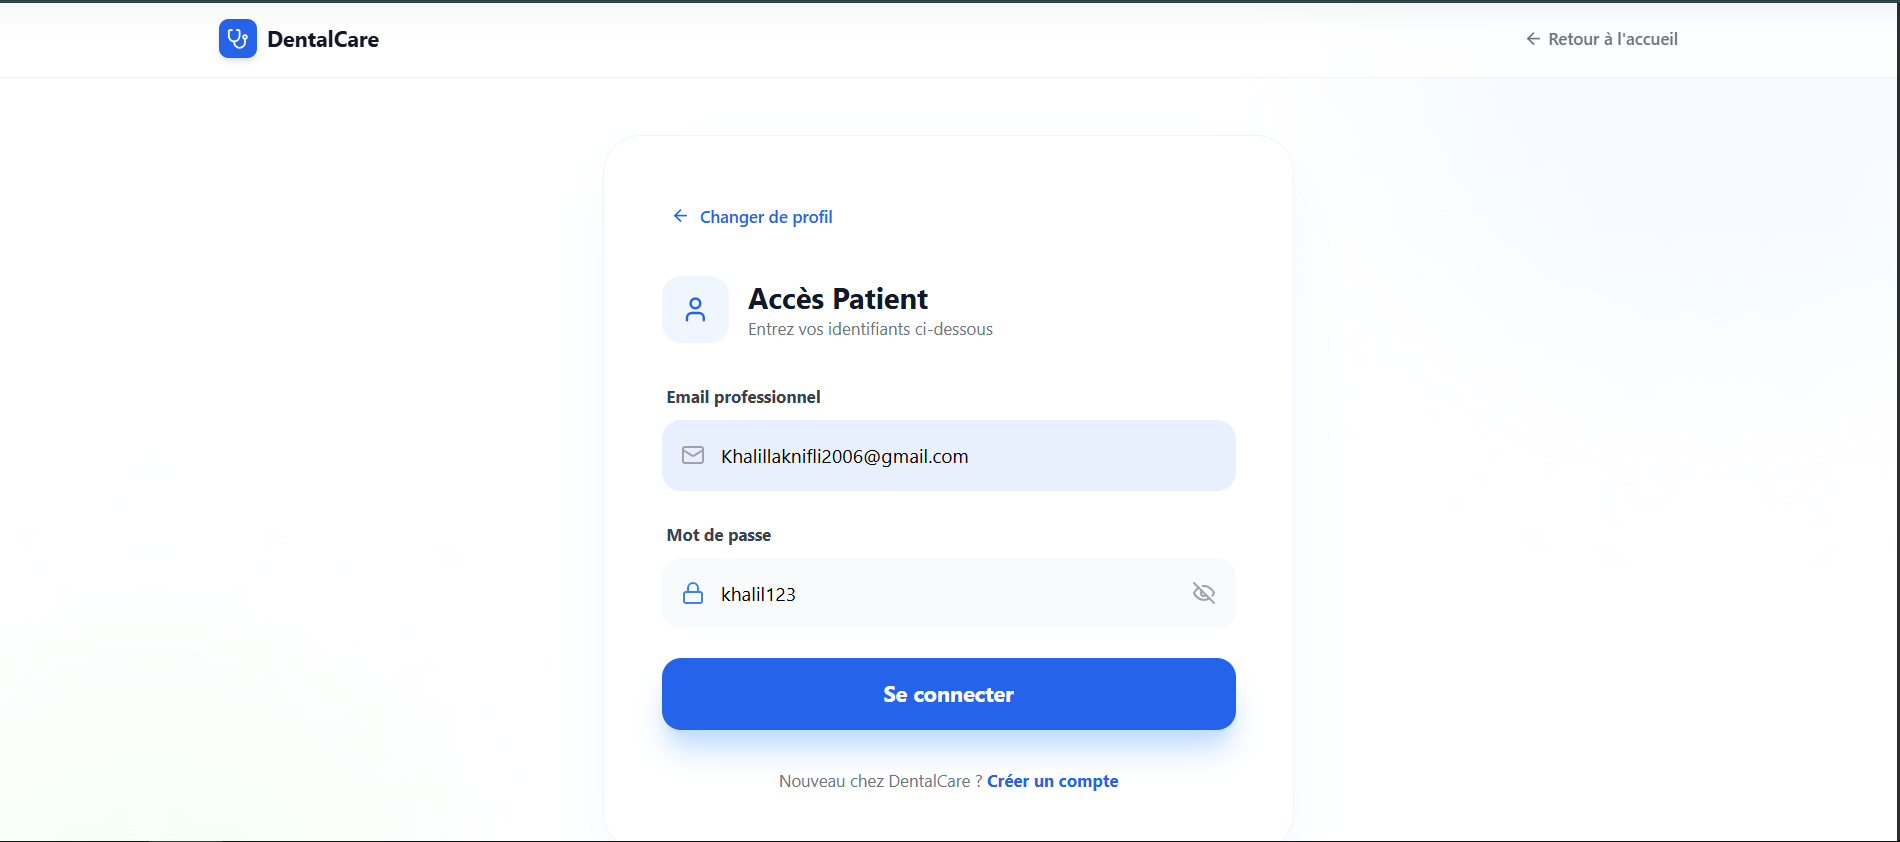
\includegraphics[width=0.9\textwidth]{login.png}
    \caption{Interface de connexion au Cabinet Dentaire}
\end{figure}

L'interface de connexion offre un système d'authentification sécurisé avec plusieurs fonctionnalités clés. L'utilisateur peut sélectionner son rôle parmi trois options : Patient, Docteur ou Personnel Administratif, ce qui permet au système de rediriger vers l'espace approprié après authentification. Le formulaire inclut des champs pour l'email et le mot de passe avec validation en temps réel. Un système de gestion d'erreurs affiche des messages clairs en cas d'échec de connexion (identifiants incorrects, compte inexistant, etc.). L'interface inclut également un lien vers la page d'inscription pour les nouveaux utilisateurs et un design centré avec une carte (card) pour une meilleure expérience utilisateur. La sécurité est assurée par l'authentification JWT côté backend, avec stockage sécurisé du token dans le localStorage du navigateur.

\begin{figure}[H]
    \centering
    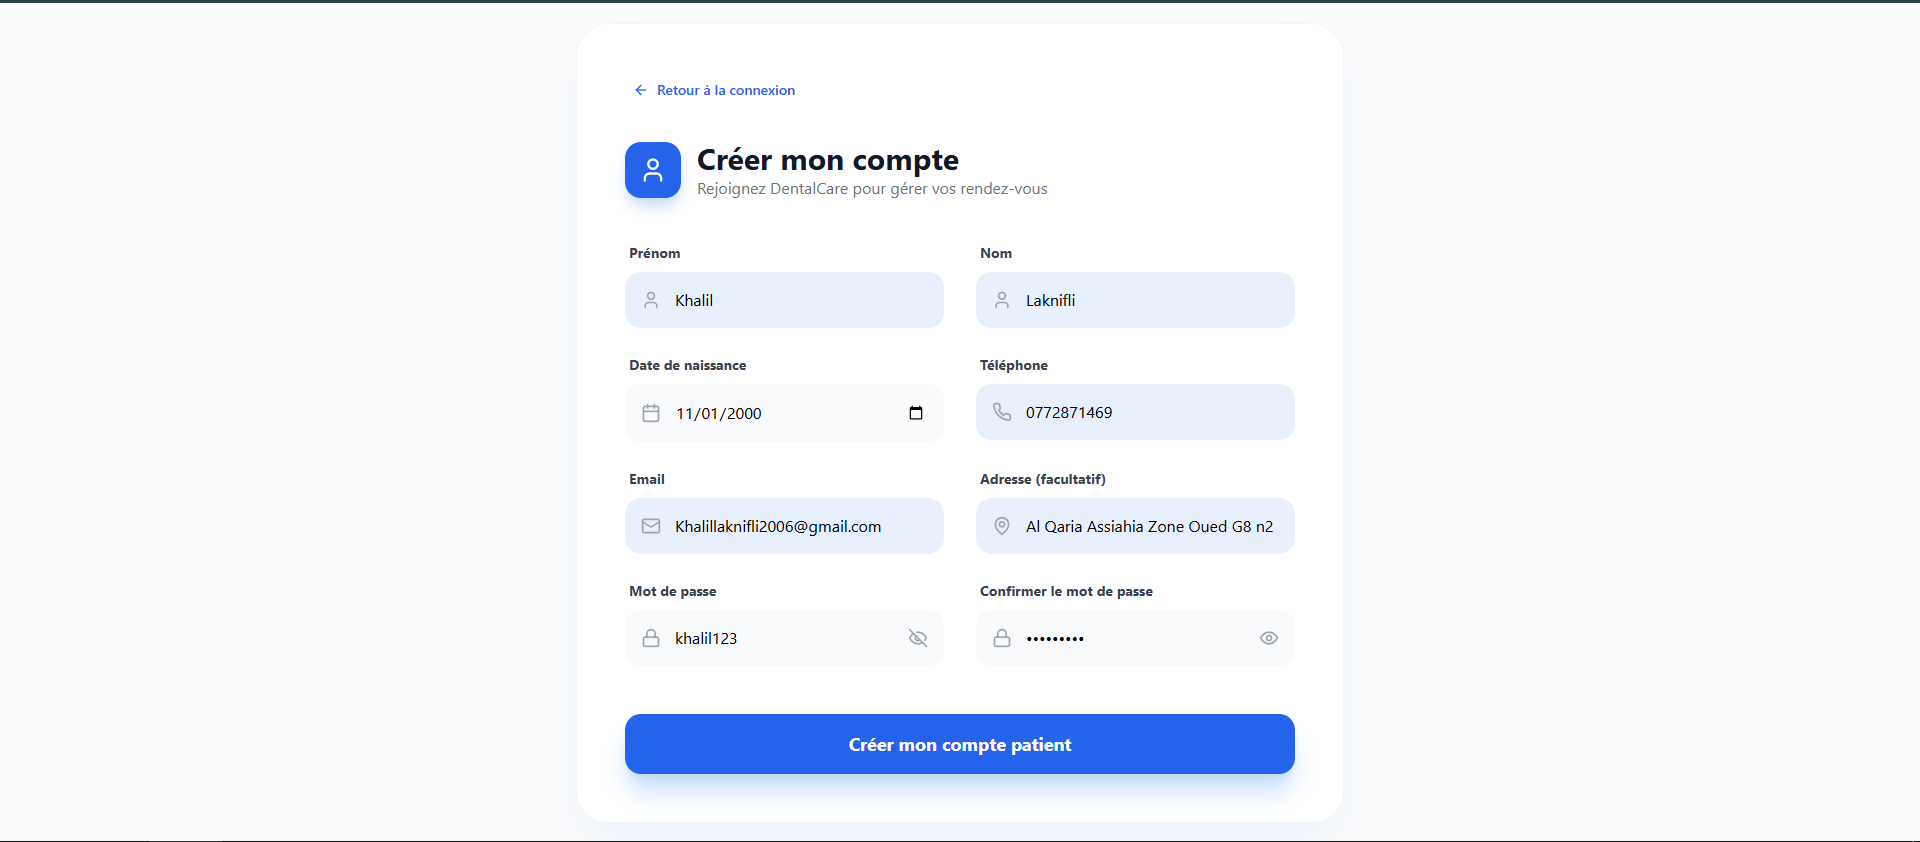
\includegraphics[width=0.9\textwidth]{signup.png}
    \caption{Interface de création de compte pour les patients}
\end{figure}

Le formulaire d'inscription permet aux nouveaux patients de créer un compte complet avec toutes les informations nécessaires. L'interface comprend plusieurs sections organisées : informations personnelles (nom, prénom, date de naissance, téléphone, adresse), informations de connexion (email avec vérification de format, mot de passe avec confirmation et indicateur de force), informations médicales (groupe sanguin, allergies multiples avec possibilité d'ajout/suppression dynamique, antécédents médicaux dans une zone de texte), et validation complète avec messages d'erreur contextuels pour chaque champ. Le formulaire utilise la validation côté client avec React pour une expérience fluide, puis une validation côté serveur via Laravel pour garantir l'intégrité des données. Après inscription réussie, le patient est automatiquement authentifié et redirigé vers son tableau de bord personnel.

\subsection{Espaces Docteur}

Le docteur dispose d'outils complets pour le suivi de son activité et de ses patients.

\begin{figure}[H]
    \centering
    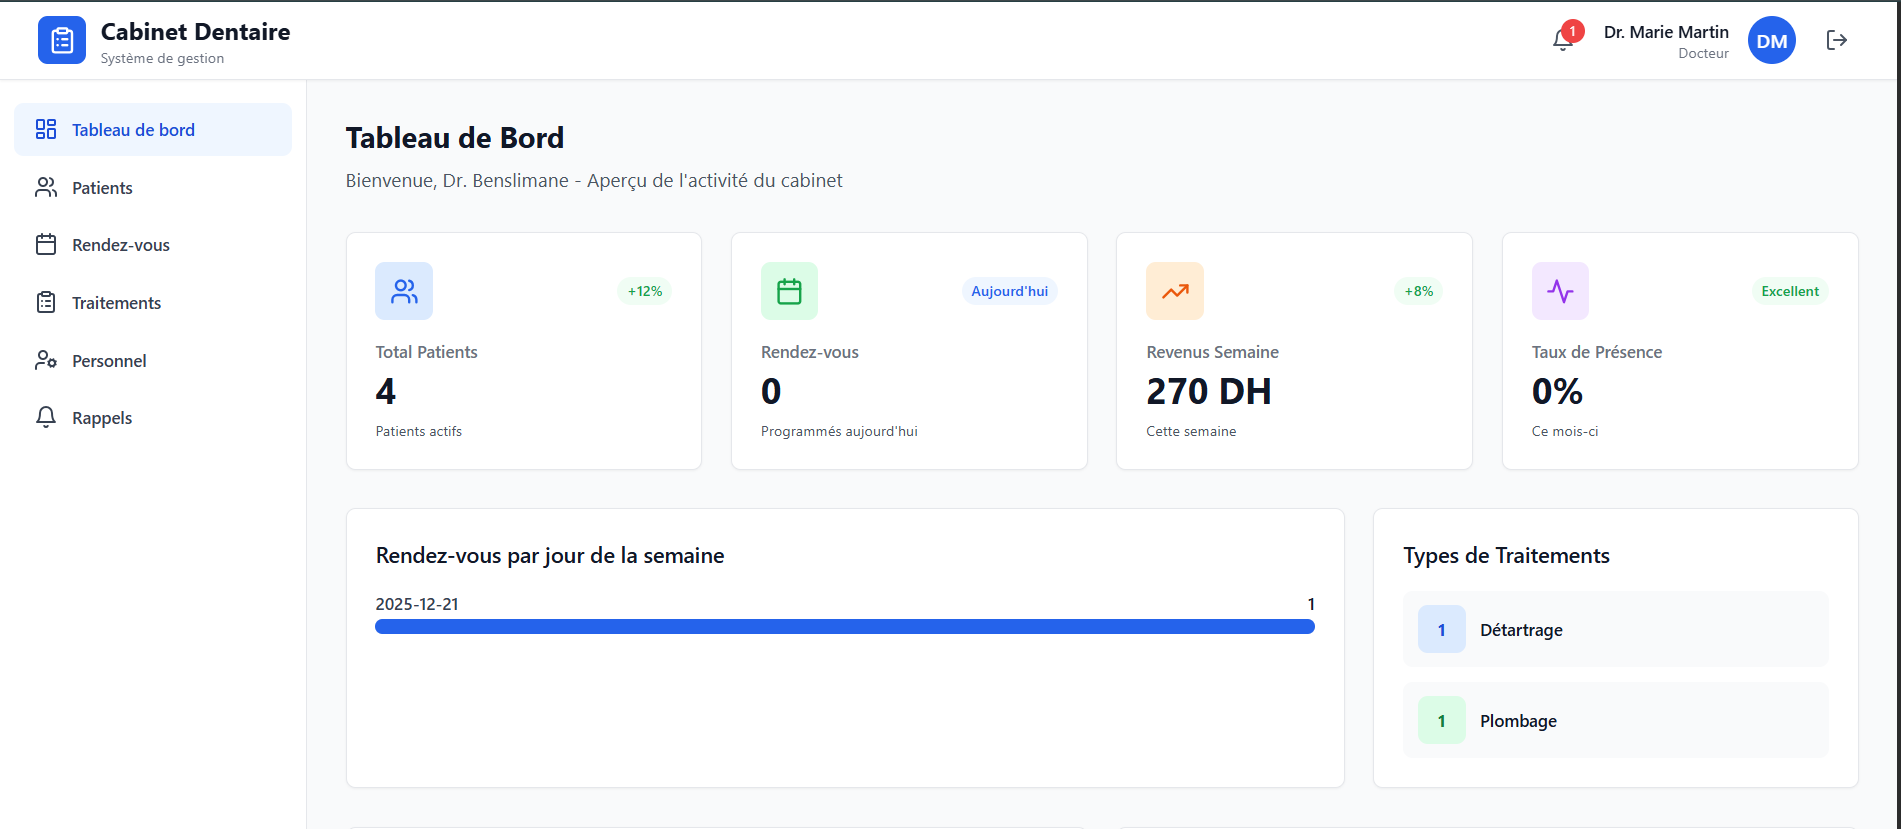
\includegraphics[width=0.9\textwidth]{Tableaudebord_PartieDocteur.png}
    \caption{Tableau de bord du docteur avec statistiques en temps réel, graphiques des rendez-vous et revenus}
\end{figure}

Le tableau de bord du docteur offre une vue d'ensemble complète de l'activité du cabinet avec des statistiques en temps réel. L'interface présente quatre cartes principales affichant les indicateurs clés : le nombre total de patients enregistrés dans le système, le nombre de rendez-vous prévus pour la journée en cours, les revenus générés sur les 7 derniers jours (calculés à partir des coûts des traitements), et le taux de complétion des rendez-vous sur les 30 derniers jours (pourcentage de rendez-vous complétés vs annulés). Un graphique linéaire montre l'évolution des rendez-vous sur les 7 derniers jours, permettant de visualiser les tendances. Un graphique en camembert présente la répartition des types de traitements les plus fréquents. La section "Rendez-vous à venir" liste les 10 prochains rendez-vous avec les informations essentielles (patient, date, heure, type). Enfin, une section "Rappels en attente" affiche les rappels qui doivent être envoyés aux patients. Toutes ces données sont récupérées dynamiquement via l'API REST et mises à jour en temps réel.

\begin{figure}[H]
    \centering
    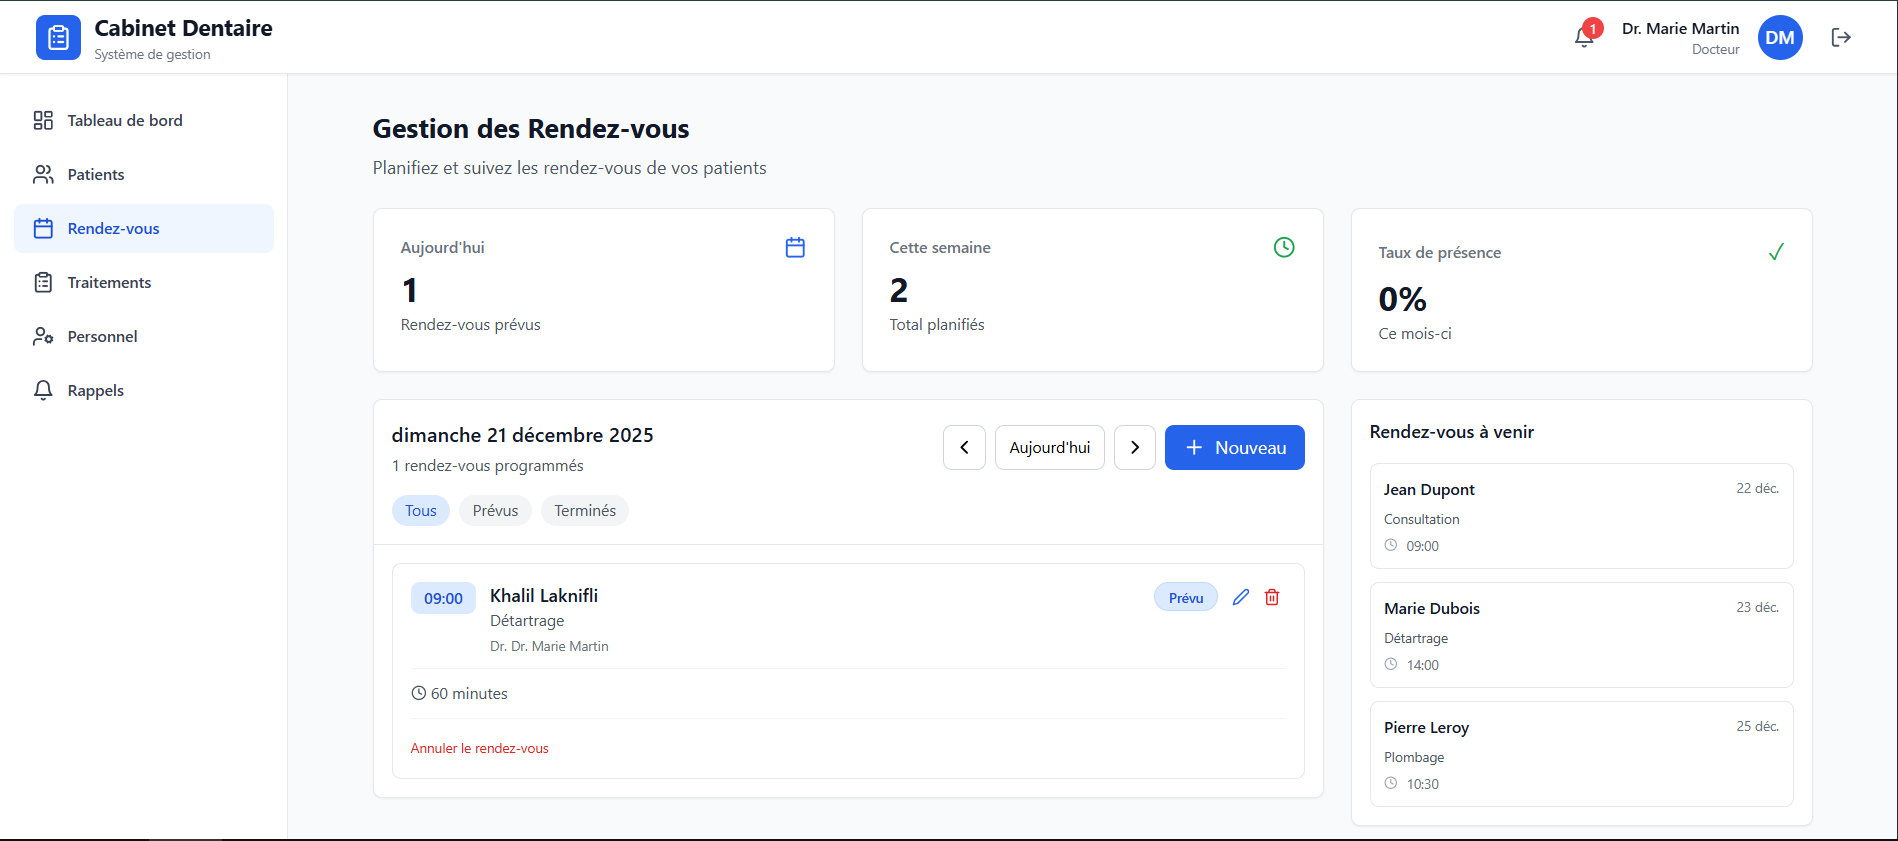
\includegraphics[width=0.9\textwidth]{GestionRendezvous_PartieDocteur.png}
    \caption{Interface de gestion des rendez-vous avec calendrier interactif (Docteur/Admin)}
\end{figure}

L'interface de gestion des rendez-vous combine un calendrier interactif et une liste détaillée pour une gestion optimale. Le calendrier mensuel permet de visualiser tous les rendez-vous avec un code couleur selon leur statut (scheduled, completed, cancelled, no-show). La navigation permet de changer de mois facilement. La liste des rendez-vous affiche toutes les informations pertinentes : nom du patient avec possibilité de cliquer pour accéder au dossier médical, nom du dentiste assigné, date et heure du rendez-vous, type de rendez-vous (Consultation, Détartrage, Extraction, etc.), statut actuel avec badge coloré, et actions disponibles (modifier, annuler, marquer comme complété). Un formulaire modal permet de créer ou modifier un rendez-vous avec sélection du patient (recherche par nom), choix du dentiste disponible, sélection de la date et de l'heure avec vérification automatique des conflits, choix du type de rendez-vous, et ajout de notes optionnelles. Le système détecte automatiquement les conflits de rendez-vous et affiche des messages d'erreur explicites si un créneau est déjà occupé.

\begin{figure}[H]
    \centering
    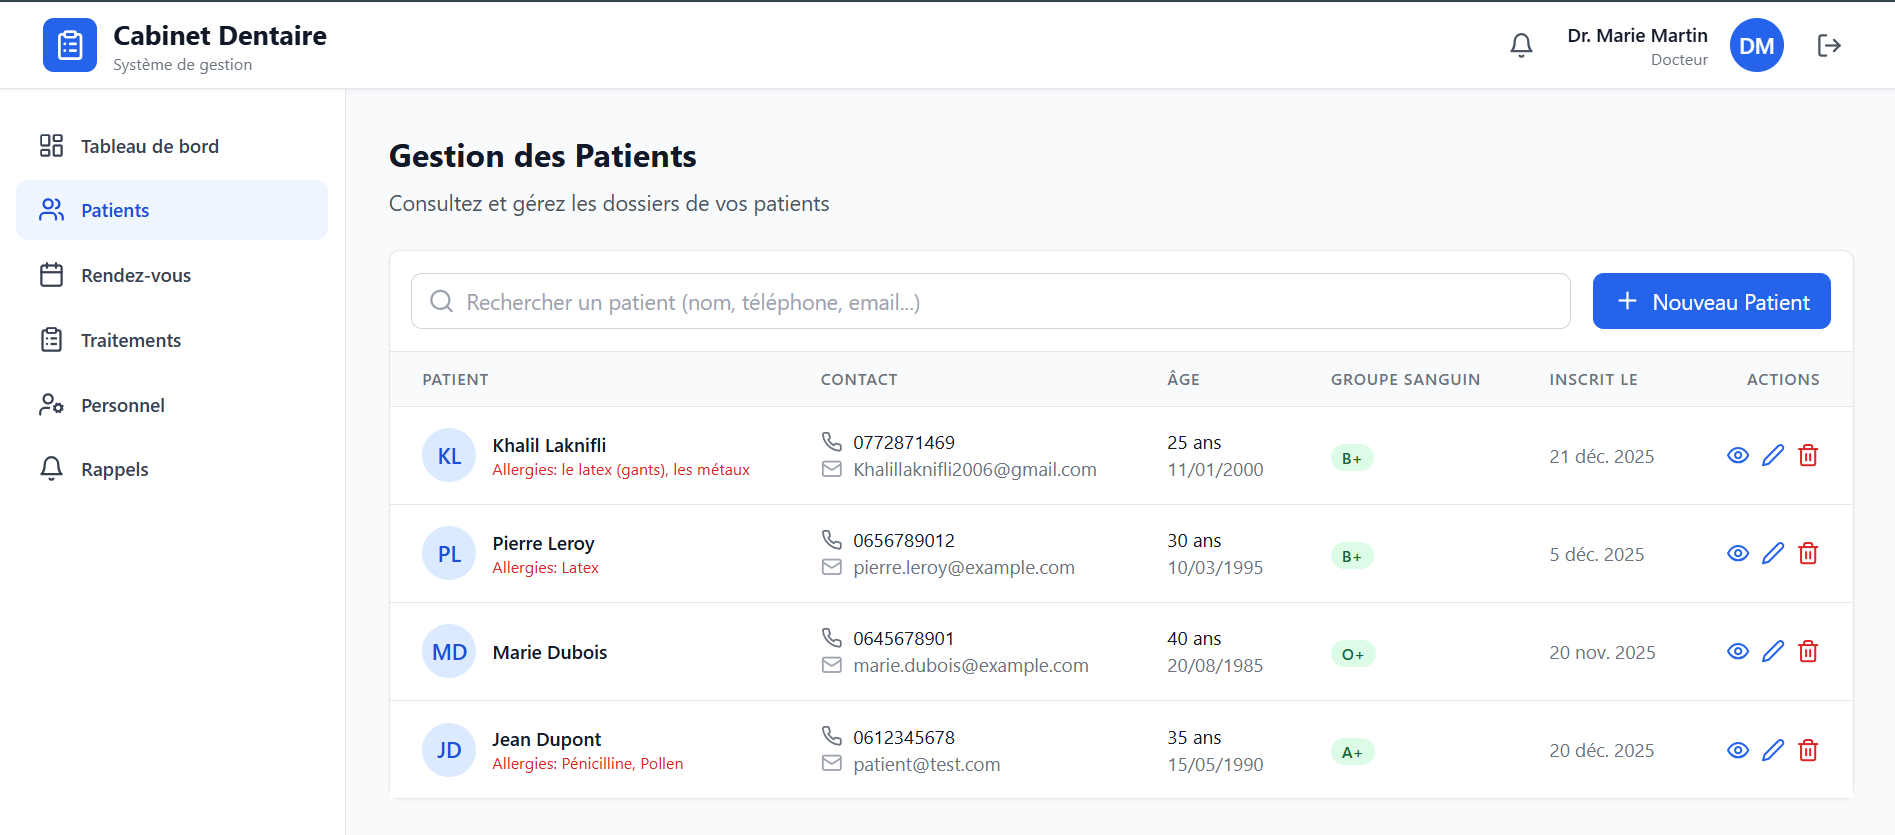
\includegraphics[width=0.9\textwidth]{Gestion_patients_PartieDocteur.png}
    \caption{Gestion complète des patients avec recherche et filtres avancés}
\end{figure}

Cette interface offre une gestion complète de la base de données des patients avec des fonctionnalités avancées de recherche et de filtrage. La barre de recherche permet de rechercher un patient par nom, prénom, email ou numéro de téléphone avec recherche en temps réel. Des filtres avancés permettent de filtrer par date d'inscription, groupe sanguin, ou présence d'allergies. La liste des patients affiche les informations essentielles : nom complet, date de naissance avec calcul automatique de l'âge, coordonnées (email, téléphone), date d'inscription, et actions rapides (voir dossier médical, modifier, supprimer). Chaque ligne est cliquable pour accéder directement au dossier médical complet du patient. Un bouton "Nouveau Patient" permet de créer un nouveau patient avec le formulaire complet. La pagination permet de naviguer dans une grande liste de patients. Les données sont chargées de manière optimisée avec pagination côté serveur pour de meilleures performances.

\begin{figure}[H]
    \centering
    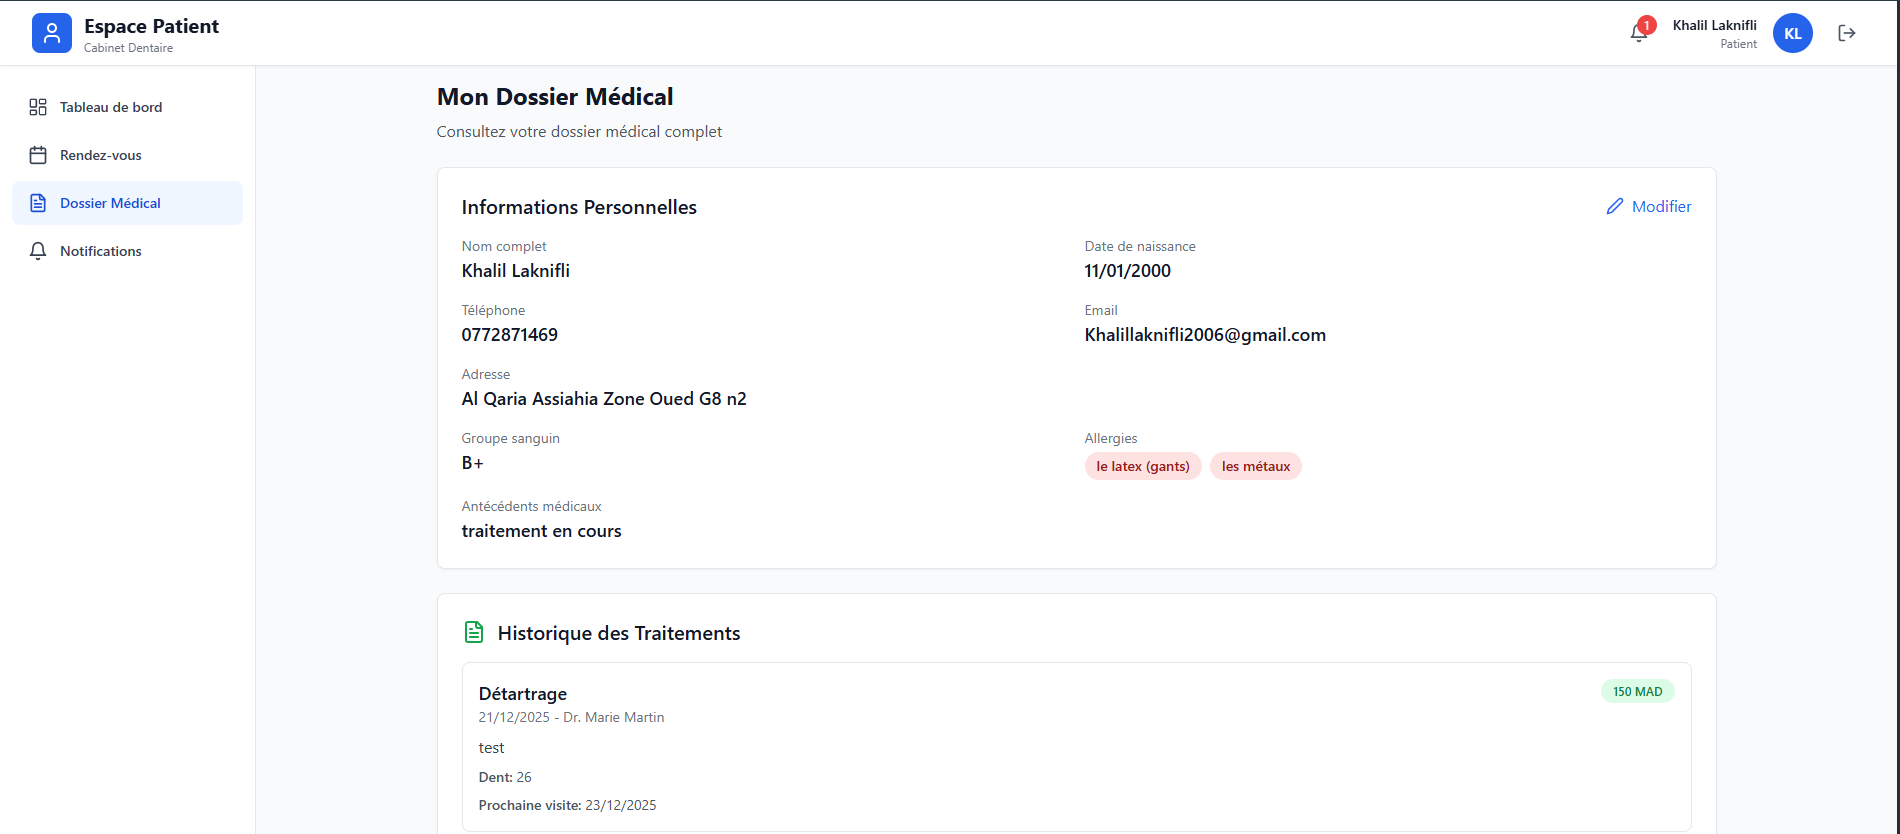
\includegraphics[width=0.9\textwidth]{DossierMedical_PartiePatient.png}
    \caption{Consultation du dossier médical d'un patient avec historique complet}
\end{figure}

Le dossier médical présente toutes les informations médicales d'un patient de manière organisée et complète. La section "Informations Personnelles" affiche les données de base : nom, prénom, date de naissance, coordonnées complètes (adresse, téléphone, email), groupe sanguin, et date d'inscription. La section "Antécédents Médicaux" présente l'historique médical du patient avec possibilité d'ajout et de modification par le docteur. La section "Allergies" liste toutes les allergies connues avec possibilité d'ajout/suppression dynamique. L'historique des rendez-vous affiche tous les rendez-vous passés et à venir avec leurs détails : date, heure, type, statut, et dentiste assigné. L'historique des traitements liste tous les traitements effectués avec leurs dates, types, descriptions détaillées, coûts, et prescriptions associées. Chaque traitement peut être consulté en détail avec ses prescriptions complètes. L'interface permet également d'ajouter rapidement un nouveau traitement directement depuis le dossier médical. Toutes les informations sont présentées de manière claire et hiérarchisée pour faciliter la consultation rapide par le professionnel de santé.

\begin{figure}[H]
    \centering
    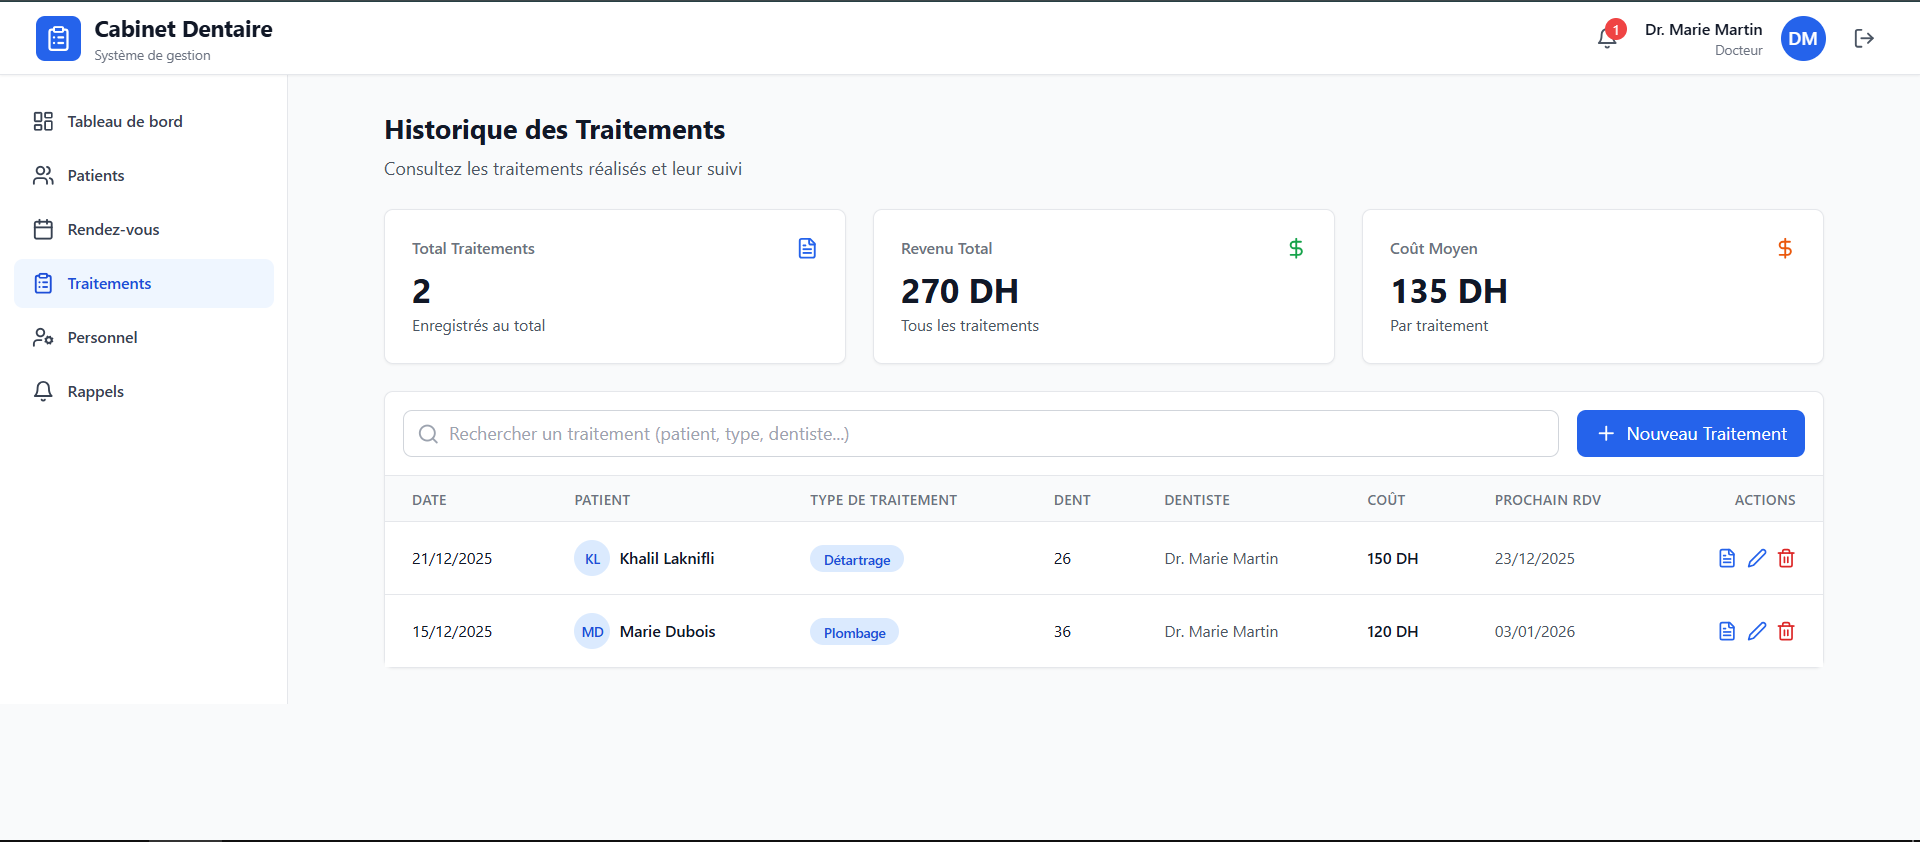
\includegraphics[width=0.9\textwidth]{HistoriqueTraitement_PartieDocteur.png}
    \caption{Historique complet des traitements effectués avec prescriptions et coûts}
\end{figure}

L'historique des traitements offre une vue complète de tous les traitements effectués dans le cabinet avec des fonctionnalités de filtrage et de recherche avancées. La liste des traitements affiche pour chaque traitement : le nom du patient avec lien vers son dossier médical, le nom du dentiste ayant effectué le traitement, la date du traitement, le type de traitement (Plombage, Détartrage, Couronne, etc.), la dent concernée (numéro ou position), le coût du traitement avec formatage monétaire, et la date de la prochaine visite recommandée si applicable. Chaque traitement peut être développé pour afficher sa description détaillée et toutes les prescriptions associées. Des filtres permettent de rechercher par patient, dentiste, type de traitement, ou période (date de début et de fin). Un graphique de statistiques montre la répartition des traitements par type et l'évolution des revenus sur une période sélectionnée. L'interface permet également d'ajouter un nouveau traitement avec un formulaire complet incluant toutes les informations nécessaires. Les prescriptions sont affichées de manière claire avec possibilité d'édition pour les traitements récents.

\subsection{Espaces Patient}

Le patient peut gérer son parcours de soin via un espace dédié.

\begin{figure}[H]
    \centering
    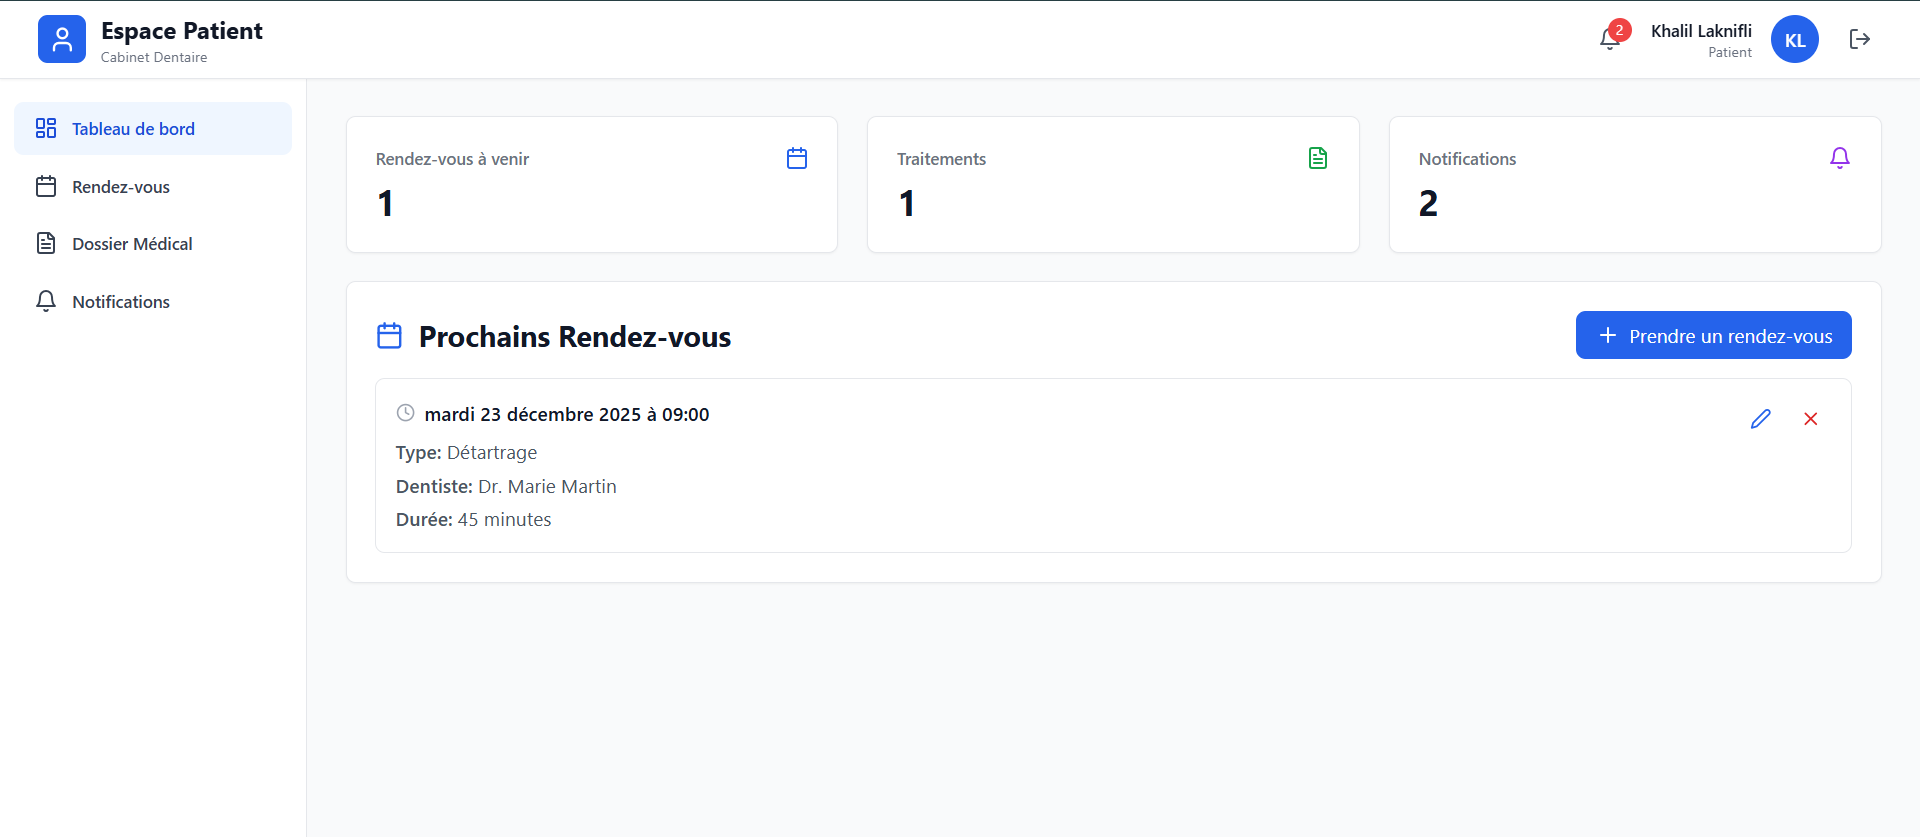
\includegraphics[width=0.9\textwidth]{tableaudebord_PartiePatient.png}
    \caption{Tableau de bord personnalisé du patient avec prochains rendez-vous et statistiques}
\end{figure}

Le tableau de bord patient offre une vue personnalisée de l'espace du patient avec des informations pertinentes et accessibles. La section "Mes Prochains Rendez-vous" affiche les rendez-vous à venir avec les détails essentiels : date et heure, nom du dentiste assigné, type de rendez-vous, et statut actuel. Chaque rendez-vous peut être modifié ou annulé directement depuis cette vue. Une section "Statistiques Personnelles" présente des indicateurs personnels : nombre total de rendez-vous effectués, nombre de traitements reçus, et date du dernier rendez-vous. Un résumé des informations personnelles permet un accès rapide aux données du compte avec possibilité de modification. Des alertes visuelles informent le patient des actions à effectuer (par exemple, confirmer un rendez-vous ou mettre à jour ses informations). L'interface est conçue pour être intuitive et rassurante, avec un design épuré et des informations clairement organisées pour faciliter la navigation.

\begin{figure}[H]
    \centering
    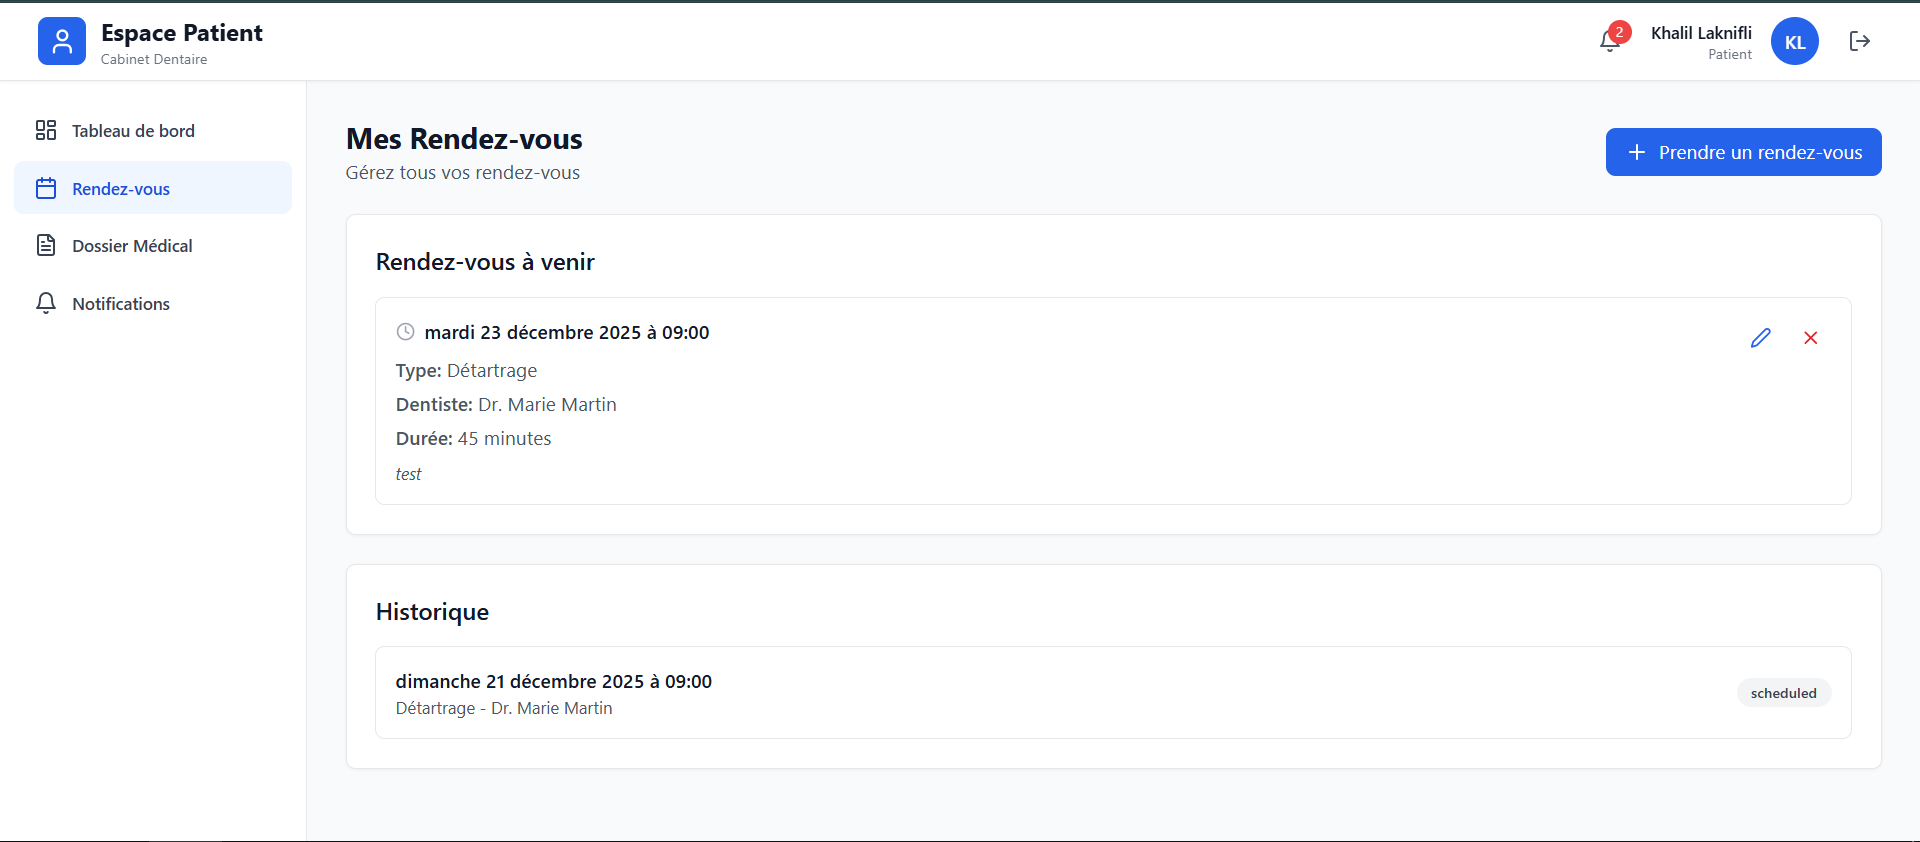
\includegraphics[width=0.9\textwidth]{rendezvous_PartiePatient.png}
    \caption{Liste et prise de rendez-vous pour le patient avec calendrier et formulaire simplifié}
\end{figure}

L'interface de gestion des rendez-vous pour le patient combine simplicité et fonctionnalité pour faciliter la prise de rendez-vous en ligne. Un calendrier mensuel interactif permet de visualiser les créneaux disponibles avec un code couleur indiquant les jours avec disponibilités. La sélection d'une date ouvre automatiquement la liste des créneaux disponibles pour cette journée. La liste des rendez-vous personnels affiche tous les rendez-vous passés et à venir avec leurs détails complets : date et heure, dentiste assigné, type de rendez-vous, statut (confirmé, complété, annulé), et actions disponibles (modifier, annuler). Un formulaire simplifié de prise de rendez-vous permet de sélectionner la date souhaitée dans un calendrier déroulant, choisir l'heure parmi les créneaux disponibles (filtrés automatiquement selon les disponibilités du dentiste), sélectionner le type de rendez-vous dans une liste déroulante, et ajouter des notes ou motifs optionnels. Le système vérifie automatiquement les conflits avant de confirmer le rendez-vous et envoie une notification de confirmation. Les rendez-vous peuvent être modifiés ou annulés jusqu'à 24 heures avant la date prévue, avec notification automatique au personnel administratif.

\begin{figure}[H]
    \centering
    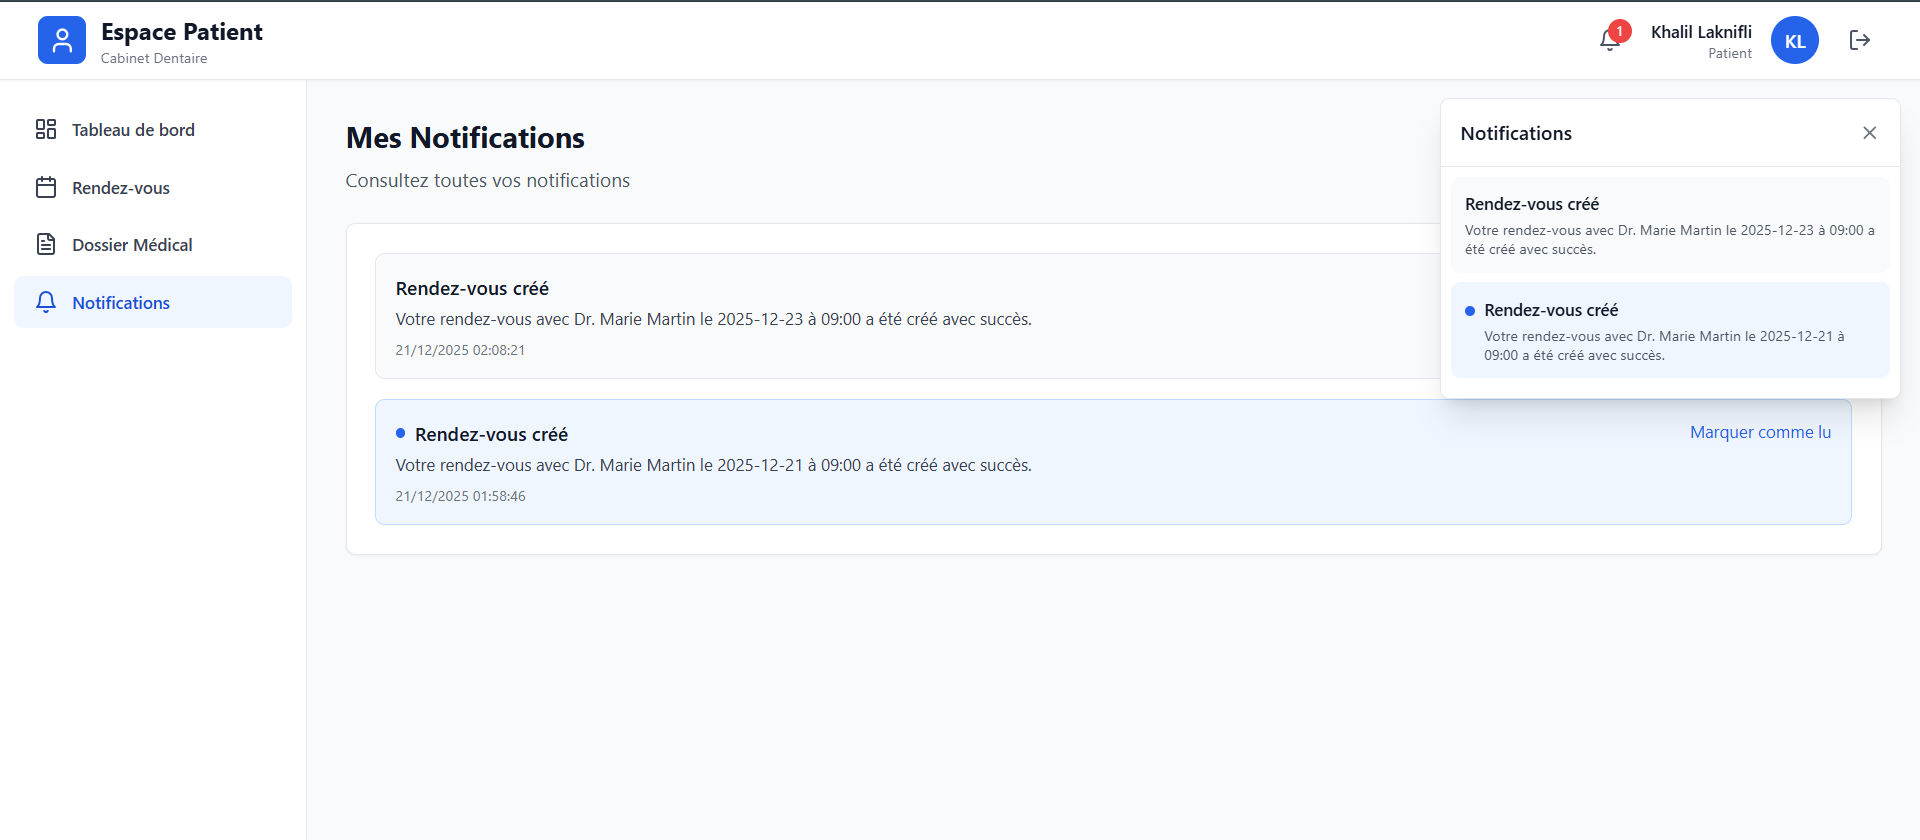
\includegraphics[width=0.9\textwidth]{Notification_PartiePatient.png}
    \caption{Système de notifications et rappels pour le patient avec marquage lu/non lu}
\end{figure}

Le système de notifications offre une communication efficace entre le cabinet et le patient avec un suivi complet des messages. La liste des notifications affiche tous les messages reçus avec leurs détails : type de notification (confirmation de rendez-vous, rappel, annulation, modification, etc.), titre et message complet, date et heure d'envoi, et statut de lecture (lu/non lu) avec badge visuel. Les notifications non lues sont mises en évidence avec un style différent et un compteur dans le menu de navigation. Chaque notification peut être marquée comme lue individuellement ou toutes les notifications peuvent être marquées comme lues en une seule action. Les notifications sont organisées par type avec des icônes distinctives pour faciliter l'identification rapide. Un système de filtrage permet d'afficher uniquement les notifications non lues, par type, ou par période. Les notifications importantes (comme les rappels de rendez-vous) sont affichées en priorité. Le système envoie automatiquement des notifications pour les événements importants : confirmation de création de rendez-vous, rappel 24h avant un rendez-vous, modification ou annulation de rendez-vous, et notifications système diverses. L'interface permet également de consulter l'historique complet des notifications pour un suivi sur le long terme.

\subsection{Gestion Administrative}

Le personnel administratif gère les ressources humaines et les rappels automatiques.

\begin{figure}[H]
    \centering
    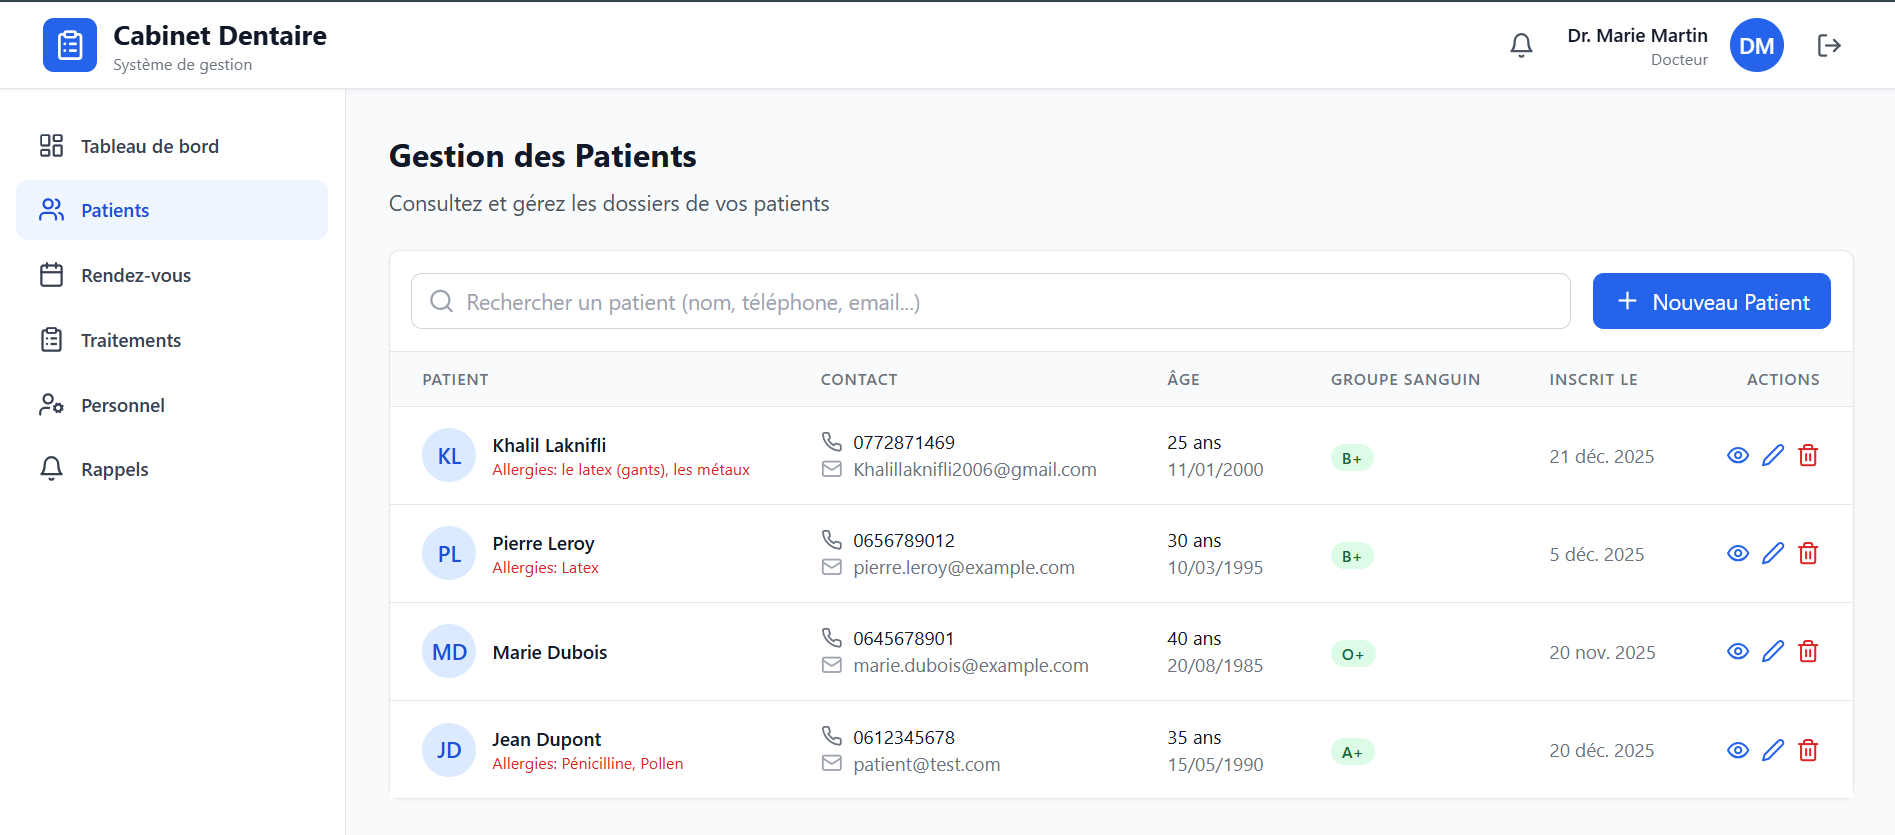
\includegraphics[width=0.9\textwidth]{Gestion_patients_PartieDocteur.png}
    \caption{Gestion complète de la base de données des patients avec CRUD complet}
\end{figure}

Cette interface de gestion administrative des patients offre toutes les fonctionnalités nécessaires pour gérer efficacement la base de données des patients. Le personnel administratif peut créer de nouveaux patients avec un formulaire complet incluant toutes les informations personnelles et médicales. La modification des informations patient est possible directement depuis la liste avec un formulaire pré-rempli. La suppression de patients est protégée par des confirmations pour éviter les suppressions accidentelles, avec vérification des contraintes (patients avec rendez-vous ou traitements ne peuvent pas être supprimés). La recherche avancée permet de trouver rapidement un patient selon plusieurs critères. L'export des données patient est disponible pour générer des rapports ou sauvegardes. L'interface affiche également des statistiques rapides : nombre total de patients, nouveaux patients du mois, et patients actifs. Toutes les actions sont tracées avec horodatage pour un suivi administratif complet.

\begin{figure}[H]
    \centering
    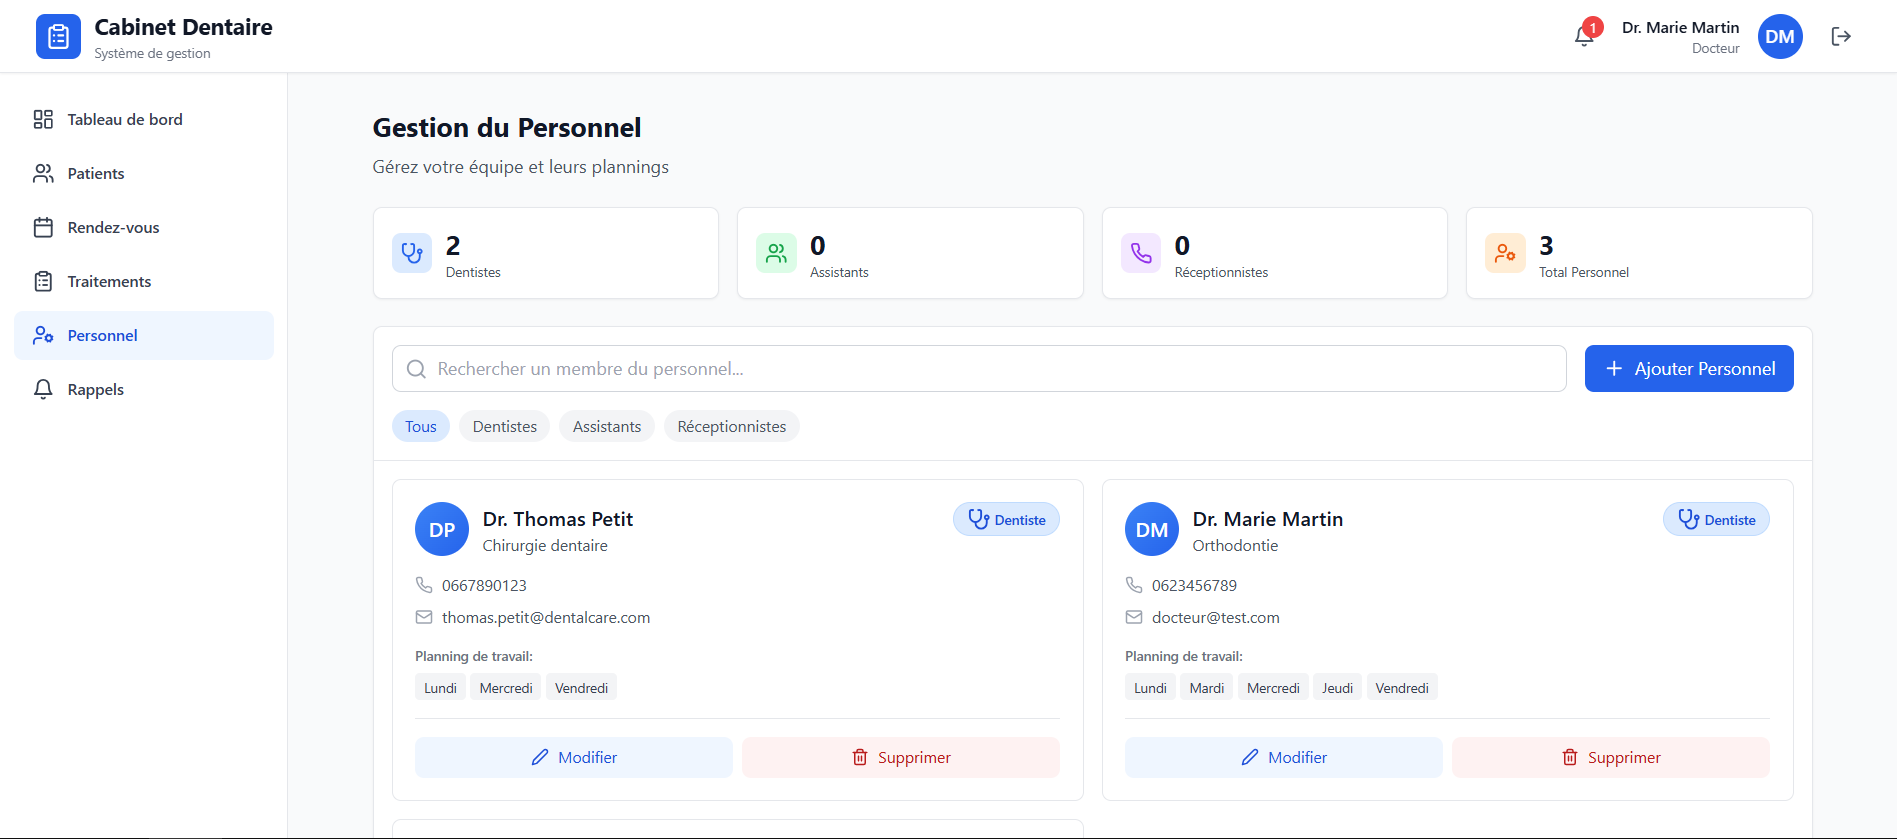
\includegraphics[width=0.9\textwidth]{GestionPersonel_PartieDocteur.png}
    \caption{Gestion des membres du personnel avec attribution de rôles et spécialités}
\end{figure}

L'interface de gestion du personnel permet aux administrateurs de gérer efficacement tous les membres du cabinet dentaire. La liste du personnel affiche tous les membres avec leurs informations essentielles : nom complet, rôle (dentiste, assistant, réceptionniste, administrateur), spécialité pour les dentistes, coordonnées (email, téléphone), et date d'embauche. Le formulaire de création/modification permet de définir toutes les informations : données personnelles (nom, prénom, date de naissance), informations de contact (email, téléphone, adresse), attribution du rôle avec sélection dans une liste déroulante, spécialité médicale pour les dentistes (orthodontie, chirurgie, etc.), et horaires de travail avec sélection des jours de la semaine. La gestion des comptes utilisateurs permet de créer automatiquement un compte de connexion pour chaque membre du personnel avec génération d'identifiants temporaires. Les permissions sont automatiquement assignées selon le rôle sélectionné. L'interface permet également de désactiver temporairement un compte sans le supprimer, utile pour les congés ou absences prolongées. Un historique des modifications est conservé pour traçabilité.

\begin{figure}[H]
    \centering
    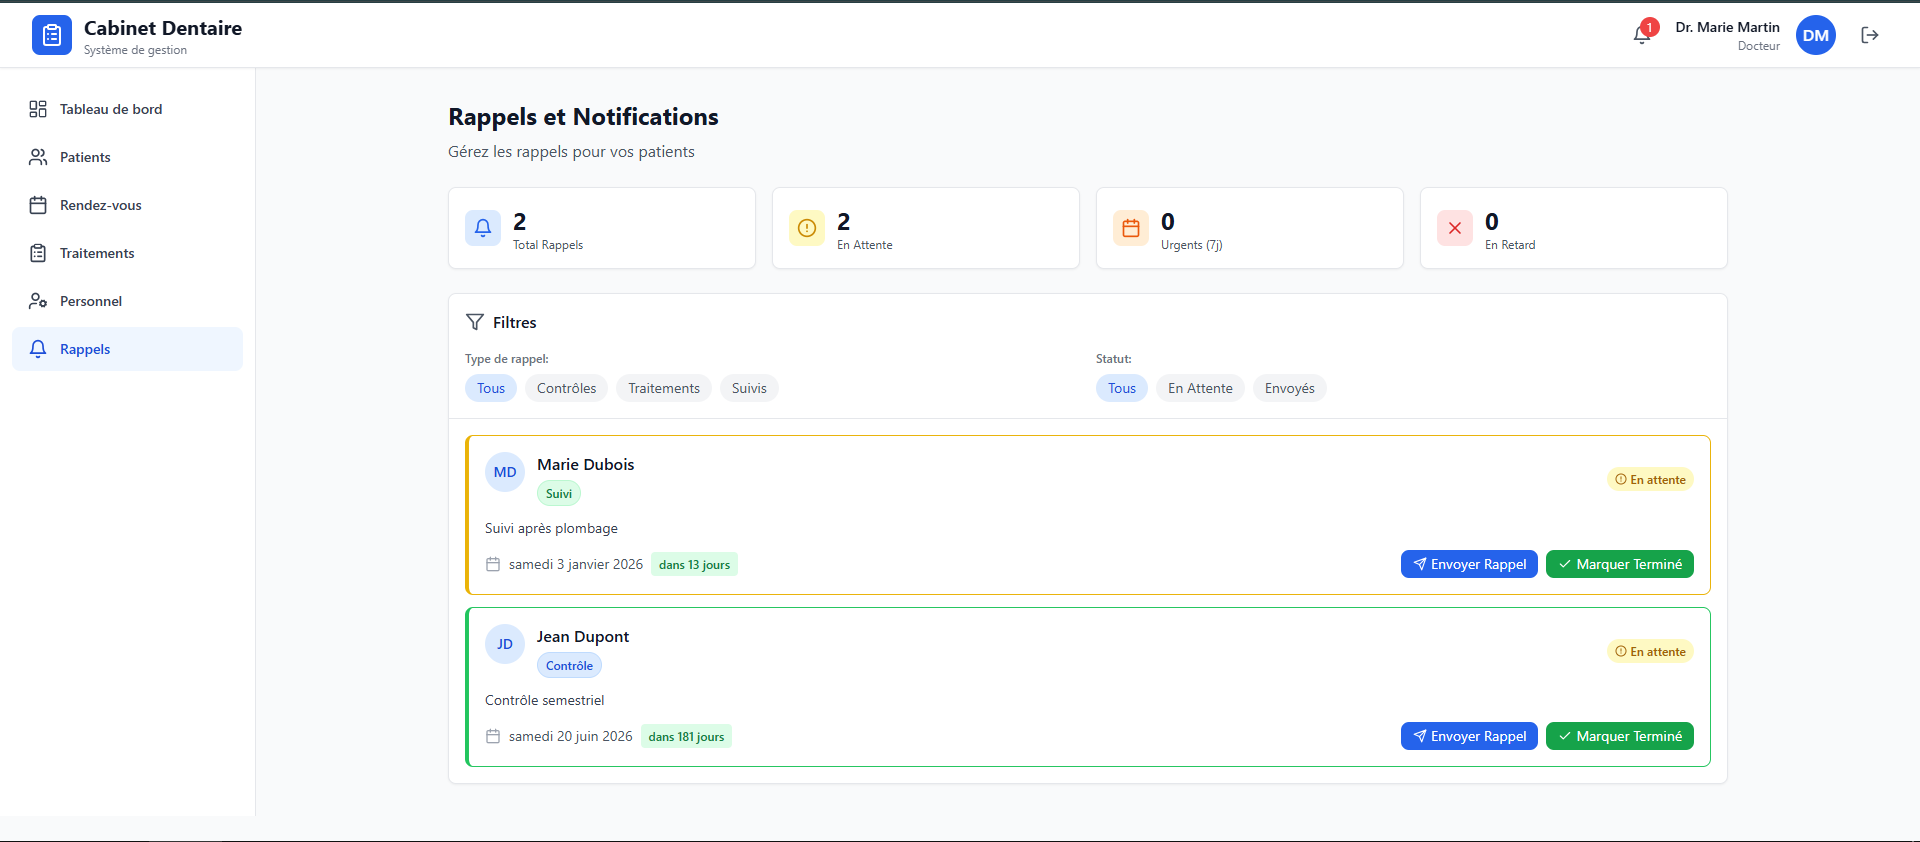
\includegraphics[width=0.9\textwidth]{RappelNotification_PartieDocteur.png}
    \caption{Tableau de bord des rappels et notifications administratives avec suivi des envois}
\end{figure}

Le tableau de bord des rappels et notifications administratives offre une vue complète du système de communication du cabinet. La section "Rappels en Attente" liste tous les rappels qui doivent être envoyés aux patients avec leurs détails : nom du patient, type de rappel (checkup, treatment, followup), date d'échéance, message du rappel, et statut (pending, sent, completed). Les rappels peuvent être envoyés manuellement ou automatiquement selon leur configuration. La section "Notifications Administratives" affiche toutes les notifications destinées au personnel administratif : nouvelles inscriptions de patients, créations/modifications/annulations de rendez-vous par les patients, et alertes système diverses. Chaque notification peut être marquée comme lue avec mise à jour automatique du compteur. Un système de filtrage permet d'afficher les notifications par type, par statut (lu/non lu), ou par période. Les statistiques affichent le nombre total de rappels envoyés, le taux de réponse aux rappels, et les notifications non lues. L'interface permet également de créer manuellement de nouveaux rappels pour des patients spécifiques avec personnalisation du message et de la date d'échéance. Un historique complet conserve toutes les notifications et rappels envoyés pour consultation ultérieure.

\section{Architecture Détaillée}

\subsection{Flux de Données}

\subsubsection{Requête Frontend → Backend}

\begin{enumerate}
    \item L'utilisateur interagit avec l'interface React
    \item Le composant appelle un service API (ex: \texttt{appointmentService.create()})
    \item Le service utilise Axios pour envoyer une requête HTTP
    \item L'intercepteur Axios ajoute automatiquement le token JWT dans l'en-tête \texttt{Authorization}
    \item La requête est envoyée à l'endpoint Laravel correspondant
\end{enumerate}

\subsubsection{Traitement Backend}

\begin{enumerate}
    \item Le middleware \texttt{auth:api} vérifie la validité du token JWT
    \item Le contrôleur reçoit la requête et valide les données avec \texttt{Validator}
    \item Le modèle Eloquent exécute les opérations sur la base de données
    \item Les relations sont chargées avec \texttt{with()} pour éviter les requêtes N+1
    \item Le contrôleur retourne une réponse JSON standardisée
\end{enumerate}

\subsubsection{Réponse Backend → Frontend}

\begin{enumerate}
    \item Axios reçoit la réponse JSON
    \item L'intercepteur gère les erreurs (401, 422, 500, etc.)
    \item Le service retourne les données au composant React
    \item Le composant met à jour son état local avec \texttt{useState}
    \item L'interface se met à jour automatiquement grâce au re-render de React
\end{enumerate}

\subsection{Gestion d'État}

\subsubsection{État Local (useState)}

Chaque composant React gère son propre état local :
\begin{itemize}
    \item Données de formulaire (valeurs saisies)
    \item État de chargement (\texttt{loading})
    \item Messages d'erreur (\texttt{error})
    \item Données affichées (liste de patients, rendez-vous, etc.)
\end{itemize}

\subsubsection{Persistance (localStorage)}

Certaines données sont persistées dans le navigateur :
\begin{itemize}
    \item Token JWT pour l'authentification
    \item Informations de l'utilisateur connecté (\texttt{currentUser})
    \item Préférences utilisateur (si implémentées)
\end{itemize}

\subsection{Optimisations Implémentées}

\subsubsection{Backend}

\begin{itemize}
    \item \textbf{Eager Loading} : Utilisation de \texttt{with()} pour charger les relations en une seule requête
    \item \textbf{Index de Base de Données} : Index sur les colonnes fréquemment interrogées (email, date, status)
    \item \textbf{Requêtes Optimisées} : Utilisation de \texttt{select()} pour limiter les colonnes récupérées
    \item \textbf{Pagination} : Possibilité d'ajouter la pagination pour les grandes listes
    \item \textbf{Cache} : Structure prête pour l'ajout de cache Redis
\end{itemize}

\subsubsection{Frontend}

\begin{itemize}
    \item \textbf{Code Splitting} : Vite divise automatiquement le code en chunks
    \item \textbf{Lazy Loading} : Possibilité d'implémenter le chargement paresseux des composants
    \item \textbf{Memoization} : Utilisation de \texttt{useMemo} et \texttt{useCallback} pour optimiser les re-renders
    \item \textbf{Débouncing} : Implémentable pour les champs de recherche
\end{itemize}

\section{Sécurité et Validation}

\subsection{Authentification JWT}

La sécurité des accès est assurée par des jetons JWT. Lors de la connexion, le backend génère un token crypté qui contient l'identité de l'utilisateur. Ce token doit être inclus dans l'entête de chaque requête protégée :

\subsubsection{Fonctionnement du JWT}

\begin{itemize}
    \item \textbf{Génération} : Lors de la connexion réussie, Laravel génère un token JWT via \texttt{tymon/jwt-auth}
    \item \textbf{Contenu} : Le token contient l'ID utilisateur, l'email, le rôle et une date d'expiration
    \item \textbf{Stockage} : Le token est stocké dans le \texttt{localStorage} du navigateur
    \item \textbf{Envoi} : Chaque requête API inclut le token dans l'en-tête \texttt{Authorization: Bearer \{token\}}
    \item \textbf{Vérification} : Le middleware \texttt{auth:api} vérifie la validité et l'expiration du token
    \item \textbf{Refresh} : Un endpoint permet de rafraîchir le token avant expiration
\end{itemize}

\subsubsection{Sécurité des Mots de Passe}

\begin{itemize}
    \item \textbf{Hachage} : Les mots de passe sont hachés avec l'algorithme BCrypt (coût 10)
    \item \textbf{Validation} : Minimum 6 caractères requis lors de l'inscription
    \item \textbf{Confirmation} : Le champ \texttt{password\_confirmation} est requis lors de l'inscription
    \item \textbf{Vérification} : \texttt{Hash::check()} compare le mot de passe saisi avec le hash stocké
\end{itemize}

\subsubsection{Gestion des Permissions}

\begin{itemize}
    \item \textbf{Rôles} : Trois rôles principaux (patient, docteur, personnelAdministratif)
    \item \textbf{Middleware} : Vérification du rôle avant l'accès aux routes spécifiques
    \item \textbf{Contrôle d'Accès} : Les patients ne peuvent accéder qu'à leurs propres données
    \item \textbf{Personnel Administratif} : Accès limité (pas d'accès aux traitements et gestion du personnel)
\end{itemize}

\subsection{Validation des Données}

Chaque entrée utilisateur est rigoureusement validée côté serveur à l'aide des \texttt{Validator} de Laravel. Cela protège le système contre :

\subsubsection{Protection contre les Injections}

\begin{itemize}
    \item \textbf{SQL Injection} : Protection via Eloquent ORM qui utilise des requêtes préparées
    \item \textbf{XSS} : Échappement automatique des données dans les réponses JSON
    \item \textbf{CSRF} : Désactivé pour l'API (remplacé par JWT)
\end{itemize}

\subsubsection{Règles de Validation}

\begin{itemize}
    \item \textbf{Types} : Vérification des types de données (string, integer, date, email, etc.)
    \item \textbf{Longueurs} : Contrôle des longueurs maximales (max:255, max:100, etc.)
    \item \textbf{Formats} : Validation des formats (email, date, UUID, etc.)
    \item \textbf{Unicité} : Vérification de l'unicité avec exclusion (ex: email unique sauf utilisateur courant)
    \item \textbf{Contraintes Métier} : Validation personnalisée (dates futures, montants positifs, etc.)
\end{itemize}

\subsubsection{Gestion des Erreurs}

\begin{itemize}
    \item \textbf{Codes HTTP} : Utilisation appropriée (200, 201, 401, 404, 422, 500)
    \item \textbf{Messages d'Erreur} : Messages explicites et traduits en français
    \item \textbf{Format Standardisé} : Réponses JSON avec champ \texttt{success} et \texttt{errors}
    \item \textbf{Logging} : Erreurs loggées côté serveur pour débogage
\end{itemize}

\section{Tests et Validation}

Le projet a été validé à travers plusieurs phases de tests rigoureuses :

\subsection{Tests Backend}

\textbf{Tests Unitaires avec PHPUnit :}
\begin{itemize}
    \item Tests des modèles Eloquent (User, Patient, Appointment, Treatment)
    \item Vérification des relations entre modèles (hasMany, belongsTo)
    \item Tests des méthodes de calcul (statistiques, taux de complétion)
    \item Validation de la logique de détection de conflits de rendez-vous
    \item Tests des contrôleurs API (codes de réponse HTTP, formats JSON)
\end{itemize}

\textbf{Tests d'Intégration :}
\begin{itemize}
    \item Tests des endpoints API avec différents rôles utilisateur
    \item Vérification du flux d'authentification JWT complet
    \item Tests de création/modification/suppression de ressources
    \item Validation des contraintes de base de données (clés étrangères, unicités)
\end{itemize}

\textbf{Tests de Validation :}
\begin{itemize}
    \item Vérification des règles de validation Laravel
    \item Tests des cas limites (données manquantes, formats invalides)
    \item Validation des contraintes métier (dates passées, conflits de rendez-vous)
\end{itemize}

\subsection{Tests Frontend}

\textbf{Tests d'Interface Utilisateur :}
\begin{itemize}
    \item Tests de réactivité (Responsive Design) sur mobile, tablette et desktop
    \item Vérification de l'affichage sur différents navigateurs (Chrome, Firefox, Safari, Edge)
    \item Tests d'accessibilité (navigation au clavier, contraste des couleurs)
\end{itemize}

\textbf{Tests de Flux Utilisateur :}
\begin{itemize}
    \item Parcours complet d'inscription patient
    \item Flux de connexion et authentification
    \item Processus de prise de rendez-vous avec vérification de disponibilité
    \item Gestion des erreurs et messages d'erreur utilisateur
    \item Navigation entre les différentes sections selon les rôles
\end{itemize}

\textbf{Tests Fonctionnels :}
\begin{itemize}
    \item Vérification de l'appel des API depuis le frontend
    \item Gestion du token JWT dans le localStorage
    \item Tests des intercepteurs Axios (ajout automatique du token, gestion d'erreurs 401)
    \item Validation des formulaires côté client
    \item Tests des composants React avec différents états
\end{itemize}

\subsection{Validation de Performance}

\begin{itemize}
    \item Temps de réponse des API (< 500ms pour les requêtes simples)
    \item Optimisation des requêtes N+1 avec \texttt{with()} et \texttt{eager loading}
    \item Utilisation d'index sur les colonnes fréquemment interrogées
    \item Tests de charge avec plusieurs utilisateurs simultanés
\end{itemize}

\subsection{Validation de Sécurité}

\begin{itemize}
    \item Vérification du hachage des mots de passe (BCrypt)
    \item Tests de protection contre les injections SQL (via Eloquent)
    \item Validation de l'authentification JWT (expiration, refresh)
    \item Tests d'accès non autorisé aux ressources protégées
    \item Vérification des permissions selon les rôles utilisateur
\end{itemize}

% Module Compilation
\chapter{Module : Analyse et Compilation}

Ce module illustre le cycle complet de compilation pour cinq fonctions critiques de notre application. Pour chaque extrait, nous détaillons les phases d'analyse lexicale, syntaxique, sémantique, ainsi que l'optimisation et la génération finale.

\section{Introduction au Module de Compilation}

Le module d'analyse et de compilation présente une étude approfondie du processus de compilation appliqué au code PHP de notre application Laravel. Cette analyse permet de comprendre comment un compilateur ou un interpréteur traite le code source pour le transformer en instructions exécutables.

Les cinq fonctions sélectionnées représentent des cas d'usage typiques d'une application web moderne :
\begin{itemize}
    \item \textbf{Code 1} : Récupération d'une ressource (pattern CRUD classique)
    \item \textbf{Code 2} : Validation et mise à jour de données utilisateur
    \item \textbf{Code 3} : Traitement par lots avec boucles et conditions
    \item \textbf{Code 4} : Logique conditionnelle complexe avec agrégations
    \item \textbf{Code 5} : Gestion de fichiers et validation de formulaires
\end{itemize}

Pour chaque fonction, nous analysons les cinq phases principales de la compilation :
\begin{enumerate}
    \item \textbf{Analyse Lexicale} : Décomposition du code source en tokens (mots-clés, identifiants, opérateurs, etc.)
    \item \textbf{Analyse Syntaxique} : Construction de l'arbre de syntaxe abstraite (AST) selon la grammaire du langage
    \item \textbf{Analyse Sémantique} : Vérification de la cohérence logique (types, portée des variables, appels de méthodes)
    \item \textbf{Optimisation} : Amélioration du code pour de meilleures performances (élimination de code mort, optimisation des boucles)
    \item \textbf{Génération de Code} : Production du code optimisé ou du bytecode final
\end{enumerate}

\section{Étude du Code 1 : Récupération d'un rendez-vous}

Cette fonction illustre un pattern CRUD classique : la récupération d'une ressource par son identifiant avec gestion d'erreur.

\subsection{Analyse de la Fonction}

\begin{lstlisting}[style=phpstyle, caption=Fonction getAppointment]
public function getAppointment($id)
{
    $appointment = Appointment::find($id);
    if (!$appointment) {
        return response()->json([
            'success' => false,
            'message' => 'Rendez-vous non trouvé'
        ], 404);
    }
    return response()->json([
        'success' => true,
        'data' => $appointment
    ]);
}
\end{lstlisting}

\subsubsection{Description Fonctionnelle}

Cette fonction implémente la récupération d'un rendez-vous par son identifiant unique. Elle suit le pattern de réponse JSON standardisé avec un champ \texttt{success} et des données ou un message d'erreur. En cas d'absence du rendez-vous, elle retourne un code HTTP 404 (Not Found).

\subsubsection{Points Techniques}

\begin{itemize}
    \item Utilisation d'Eloquent ORM avec la méthode statique \texttt{find()}
    \item Gestion d'erreur avec vérification de nullité
    \item Réponse JSON standardisée avec code HTTP approprié
    \item Pattern de retour cohérent pour l'API REST
\end{itemize}

\begin{figure}[H]
    \centering
    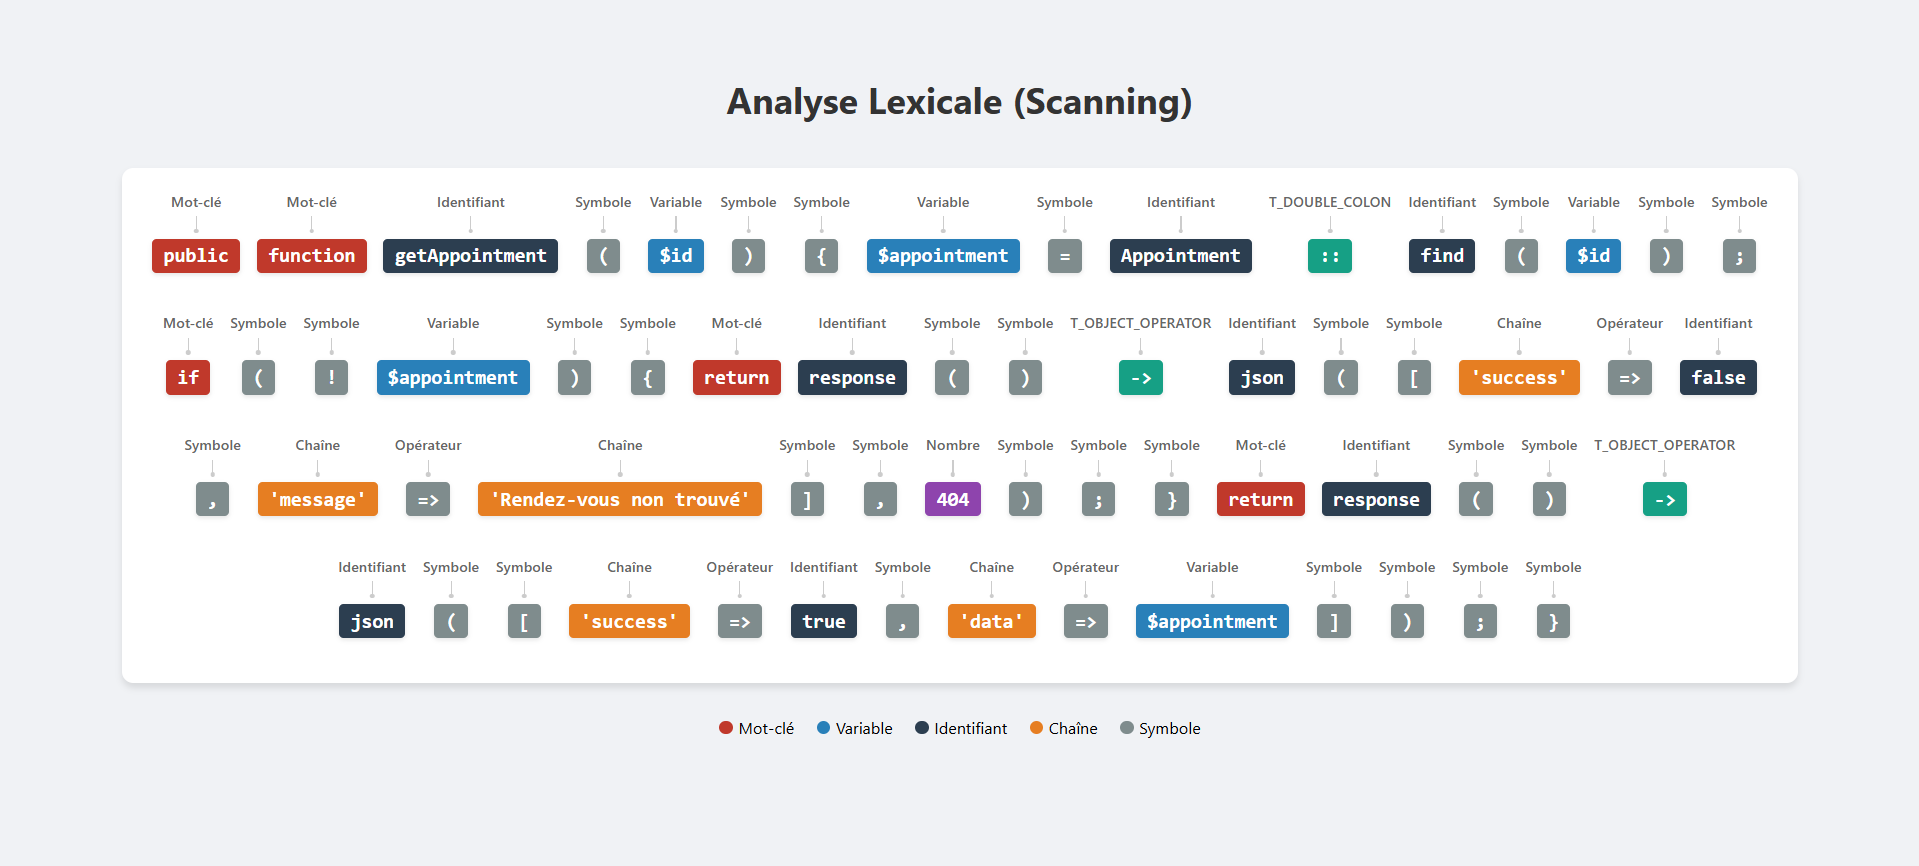
\includegraphics[width=0.7\textwidth]{analyse_lexical_code1.png}
    \caption{Analyse Lexicale (Tokens) - Code 1}
\end{figure}

\begin{figure}[H]
    \centering
    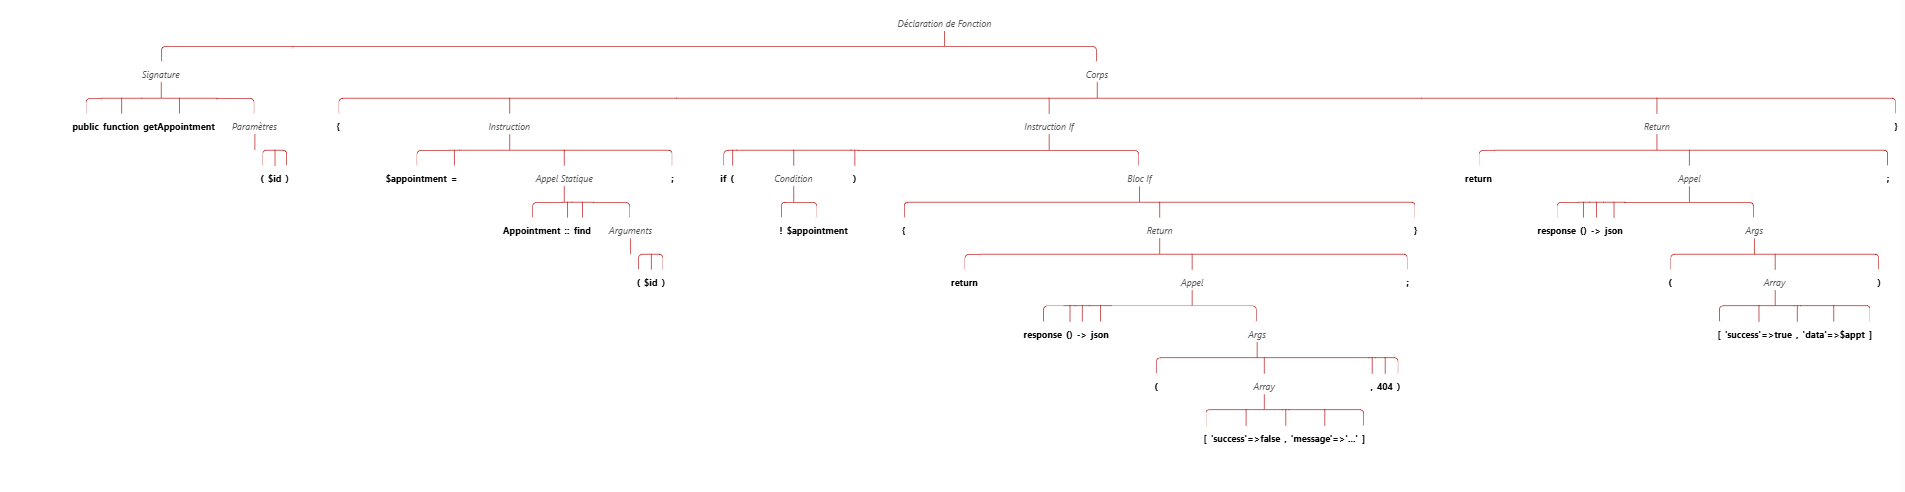
\includegraphics[width=0.8\textwidth]{analyse_syntaxique_code1.png}
    \caption{Analyse Syntaxique - Code 1}
\end{figure}

\begin{figure}[H]
    \centering
    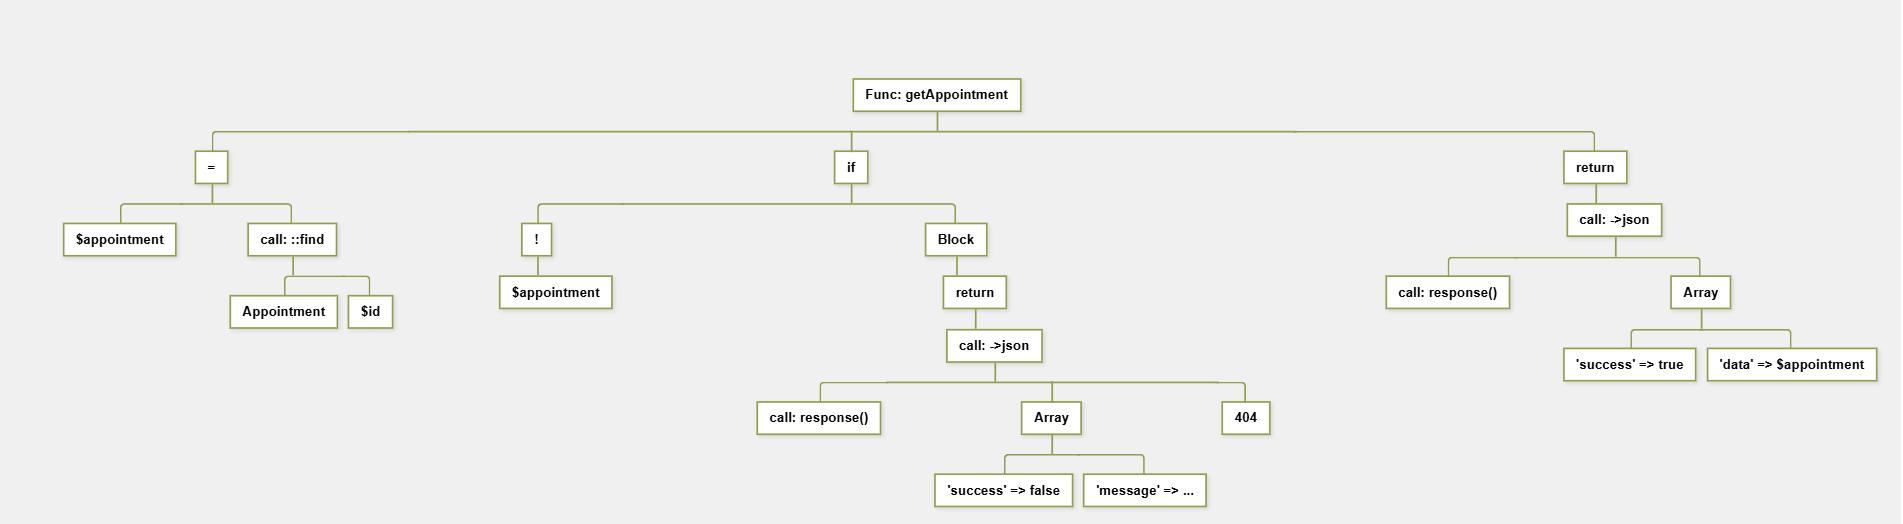
\includegraphics[width=0.8\textwidth]{analyse_sementique_code1.png}
    \caption{Analyse Sémantique - Code 1}
\end{figure}

\begin{figure}[H]
    \centering
    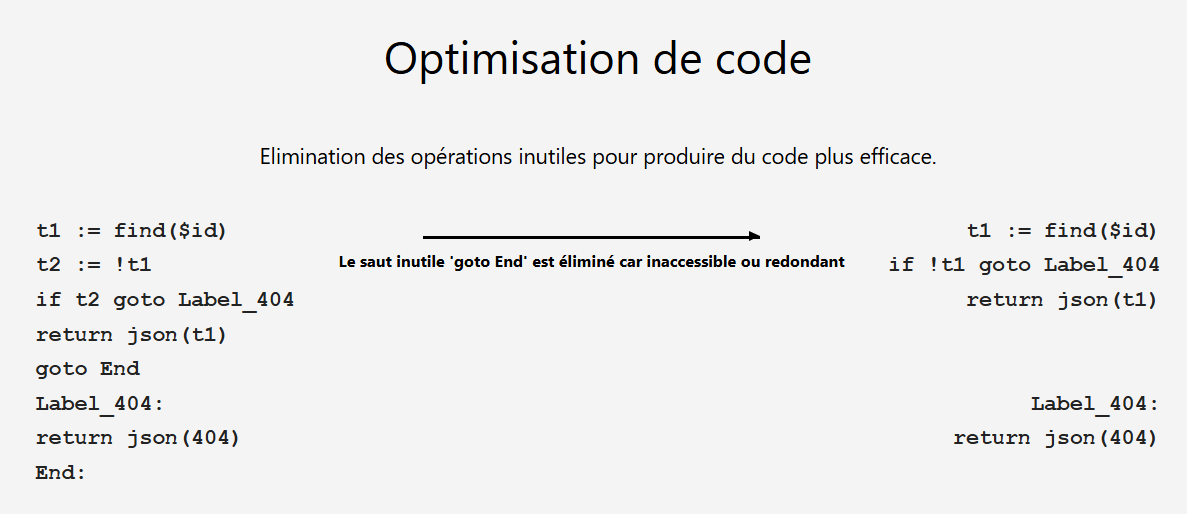
\includegraphics[width=0.8\textwidth]{optimisation_code1.png}
    \caption{Optimisation - Code 1}
\end{figure}

\begin{figure}[H]
    \centering
    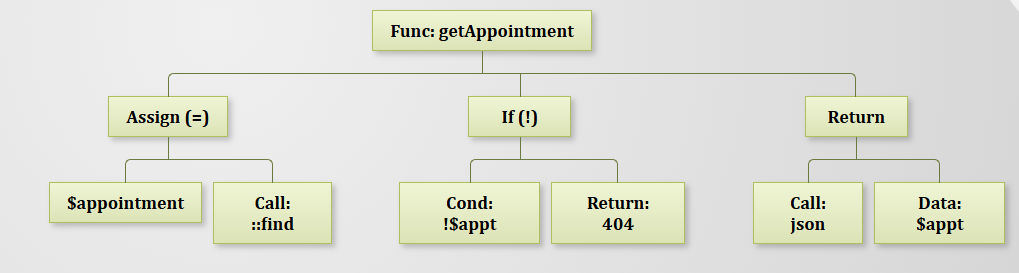
\includegraphics[width=0.8\textwidth]{generation_code1.png}
    \caption{Génération de Code - Code 1}
\end{figure}

\newpage
\section{Étude du Code 2 : Mise à jour du profil}

Cette fonction illustre la validation de données et la mise à jour d'un profil utilisateur avec des règles de validation complexes.

\subsection{Analyse de la Fonction}

\begin{lstlisting}[style=phpstyle, caption=Extrait de la fonction updateProfile]
public function updateProfile(Request $request)
{
    $validator = Validator::make($request->all(), [
        'name' => 'required|string|max:255',
        'email' => 'required|email|unique:users,email,' . auth()->id(),
        'phone' => 'nullable|string|max:20'
    ]);
    if ($validator->fails()) {
        return response()->json(['success' => false]);
    }
\end{lstlisting}

\subsubsection{Description Fonctionnelle}

Cette fonction gère la mise à jour du profil utilisateur avec validation stricte des données d'entrée. Elle utilise le système de validation de Laravel avec des règles personnalisées, notamment pour l'unicité de l'email (en excluant l'utilisateur courant).

\subsubsection{Points Techniques}

\begin{itemize}
    \item Utilisation du Validator de Laravel avec règles multiples
    \item Règle \texttt{unique} avec exclusion de l'utilisateur courant via \texttt{auth()->id()}
    \item Champs optionnels avec \texttt{nullable}
    \item Validation des types et longueurs maximales
    \item Gestion d'erreur simplifiée (retour immédiat en cas d'échec)
\end{itemize}

\begin{figure}[H]
    \centering
    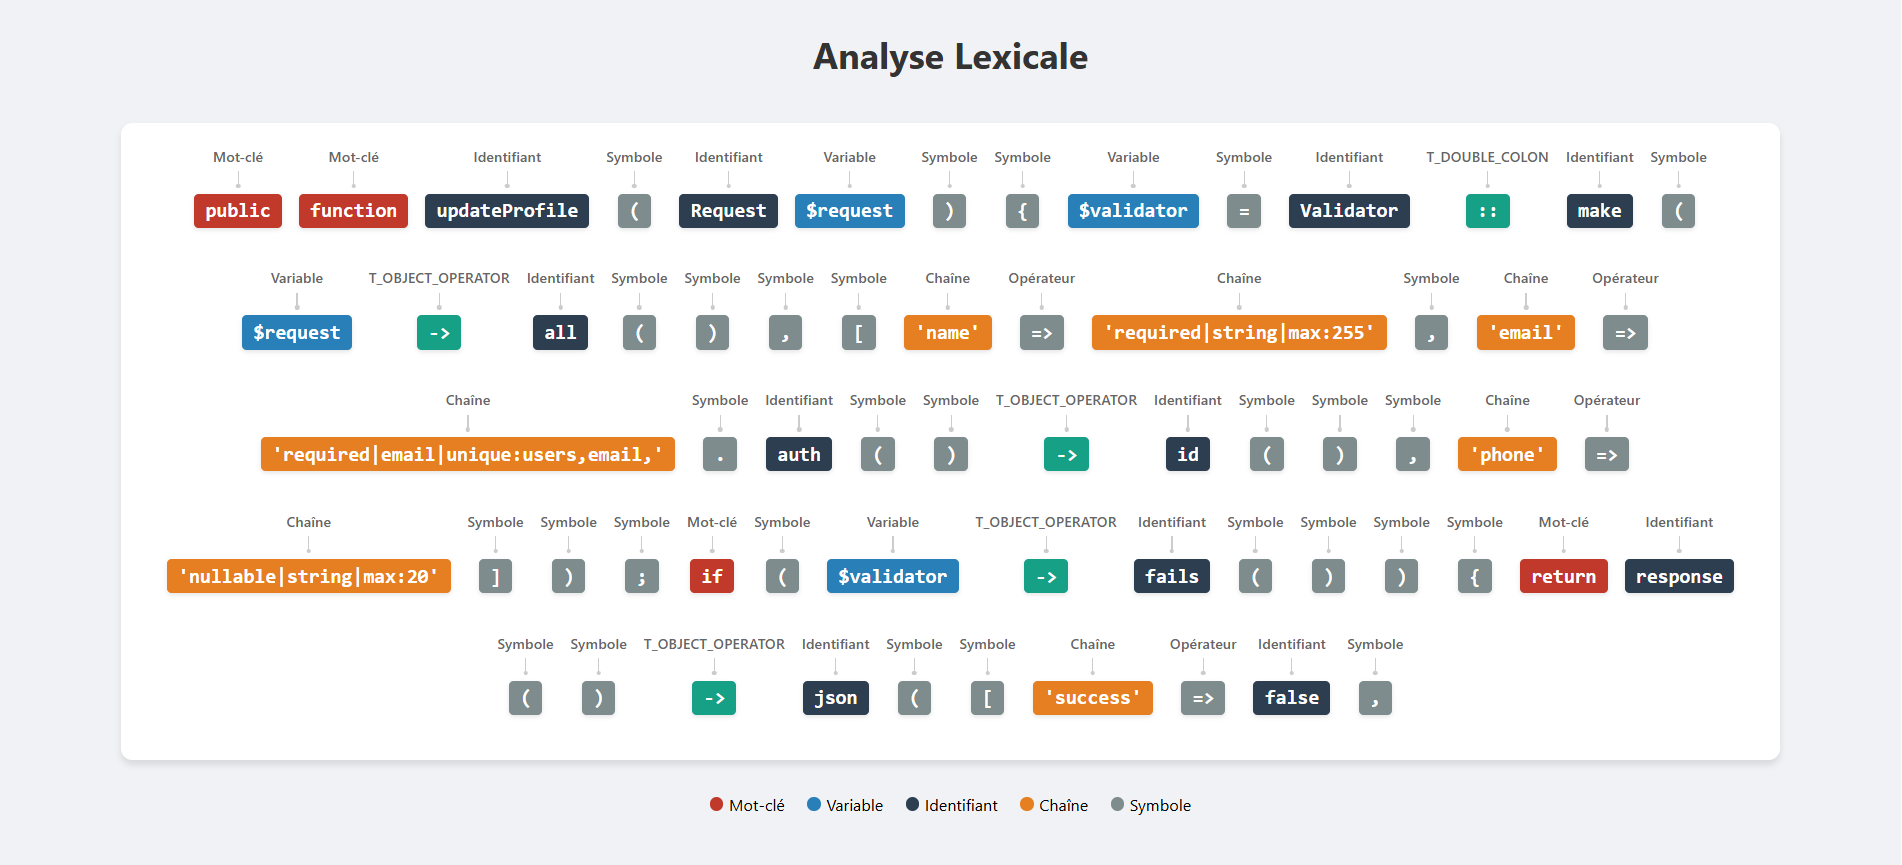
\includegraphics[width=0.7\textwidth]{analyse_lexical_code2.png}
    \caption{Analyse Lexicale - Code 2}
\end{figure}

\begin{figure}[H]
    \centering
    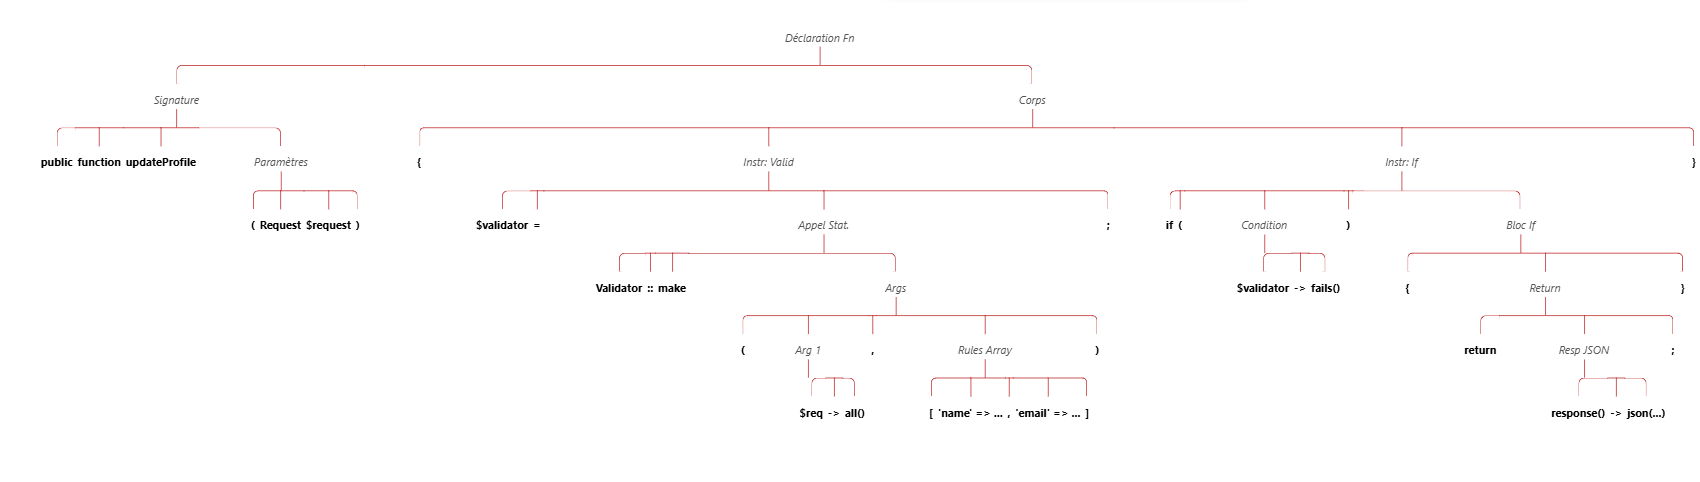
\includegraphics[width=0.8\textwidth]{analyse_syntaxique_code2.png}
    \caption{Analyse Syntaxique - Code 2}
\end{figure}

\begin{figure}[H]
    \centering
    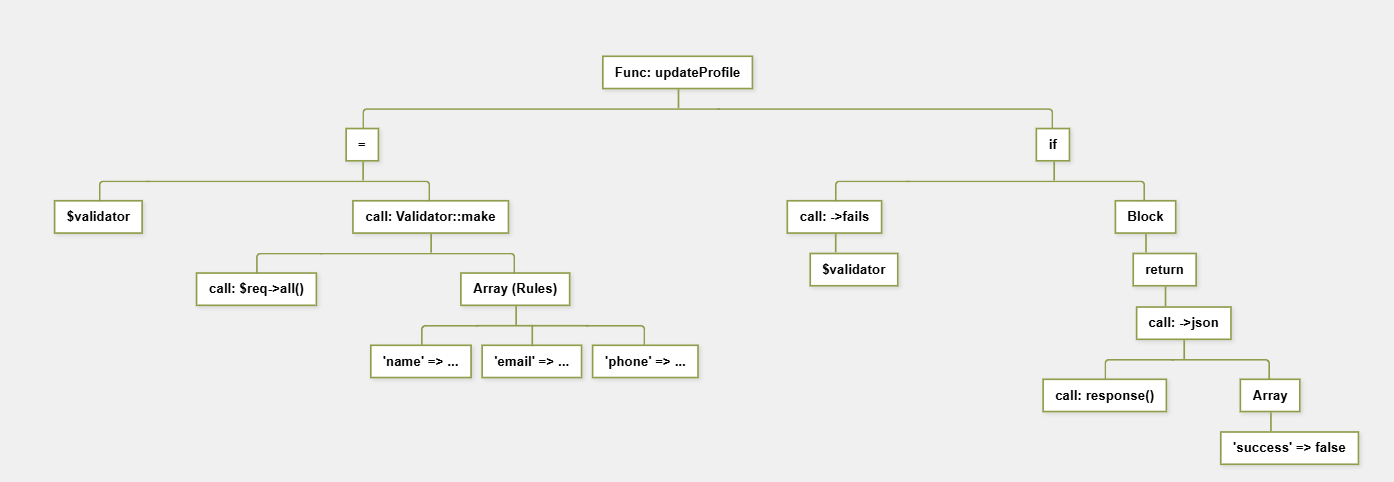
\includegraphics[width=0.8\textwidth]{analyse_sementique_code2.png}
    \caption{Analyse Sémantique - Code 2}
\end{figure}

\begin{figure}[H]
    \centering
    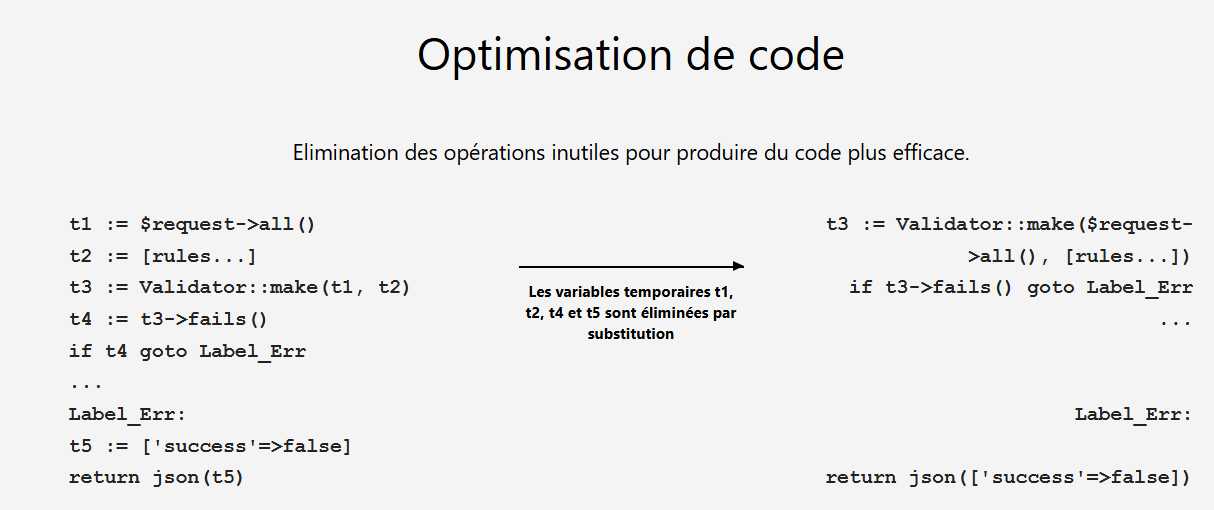
\includegraphics[width=0.8\textwidth]{optimisation_code2.png}
    \caption{Optimisation - Code 2}
\end{figure}

\begin{figure}[H]
    \centering
    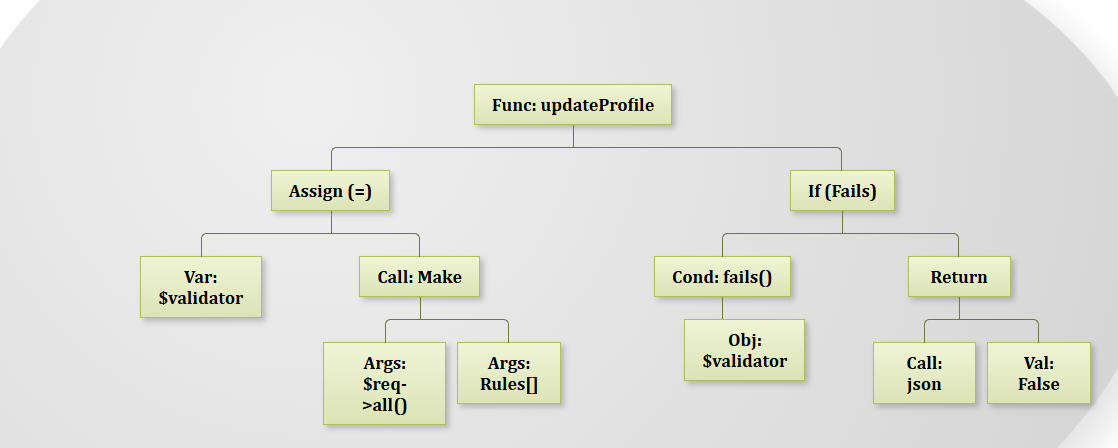
\includegraphics[width=0.8\textwidth]{generation_code2.png}
    \caption{Génération de Code - Code 2}
\end{figure}

\newpage
\section{Étude du Code 3 : Traitement des paiements}

Cette fonction illustre le traitement par lots avec requêtes filtrées, boucles et conditions multiples.

\subsection{Analyse de la Fonction}

\begin{lstlisting}[style=phpstyle, caption=Fonction processPayments]
public function processPayments()
{
    $unpaidInvoices = Invoice::where('status', 'unpaid')
                           ->where('due_date', '<', now())
                           ->get();
    foreach ($unpaidInvoices as $invoice) {
        if ($invoice->amount > 0) {
            $this->sendPaymentReminder($invoice);
            $invoice->reminder_sent_at = now();
            $invoice->save();
        }
    }
}
\end{lstlisting}

\subsubsection{Description Fonctionnelle}

Cette fonction traite les factures impayées en envoyant des rappels automatiques. Elle utilise le Query Builder d'Eloquent pour filtrer les factures non payées et échues, puis itère sur chaque facture pour envoyer un rappel si le montant est supérieur à zéro.

\subsubsection{Points Techniques}

\begin{itemize}
    \item Chaînage de méthodes \texttt{where()} pour filtres multiples
    \item Utilisation de \texttt{now()} pour les comparaisons de dates
    \item Boucle \texttt{foreach} avec traitement conditionnel
    \item Mise à jour de modèle avec \texttt{save()}
    \item Pattern de traitement par lots (batch processing)
\end{itemize}

\begin{figure}[H]
    \centering
    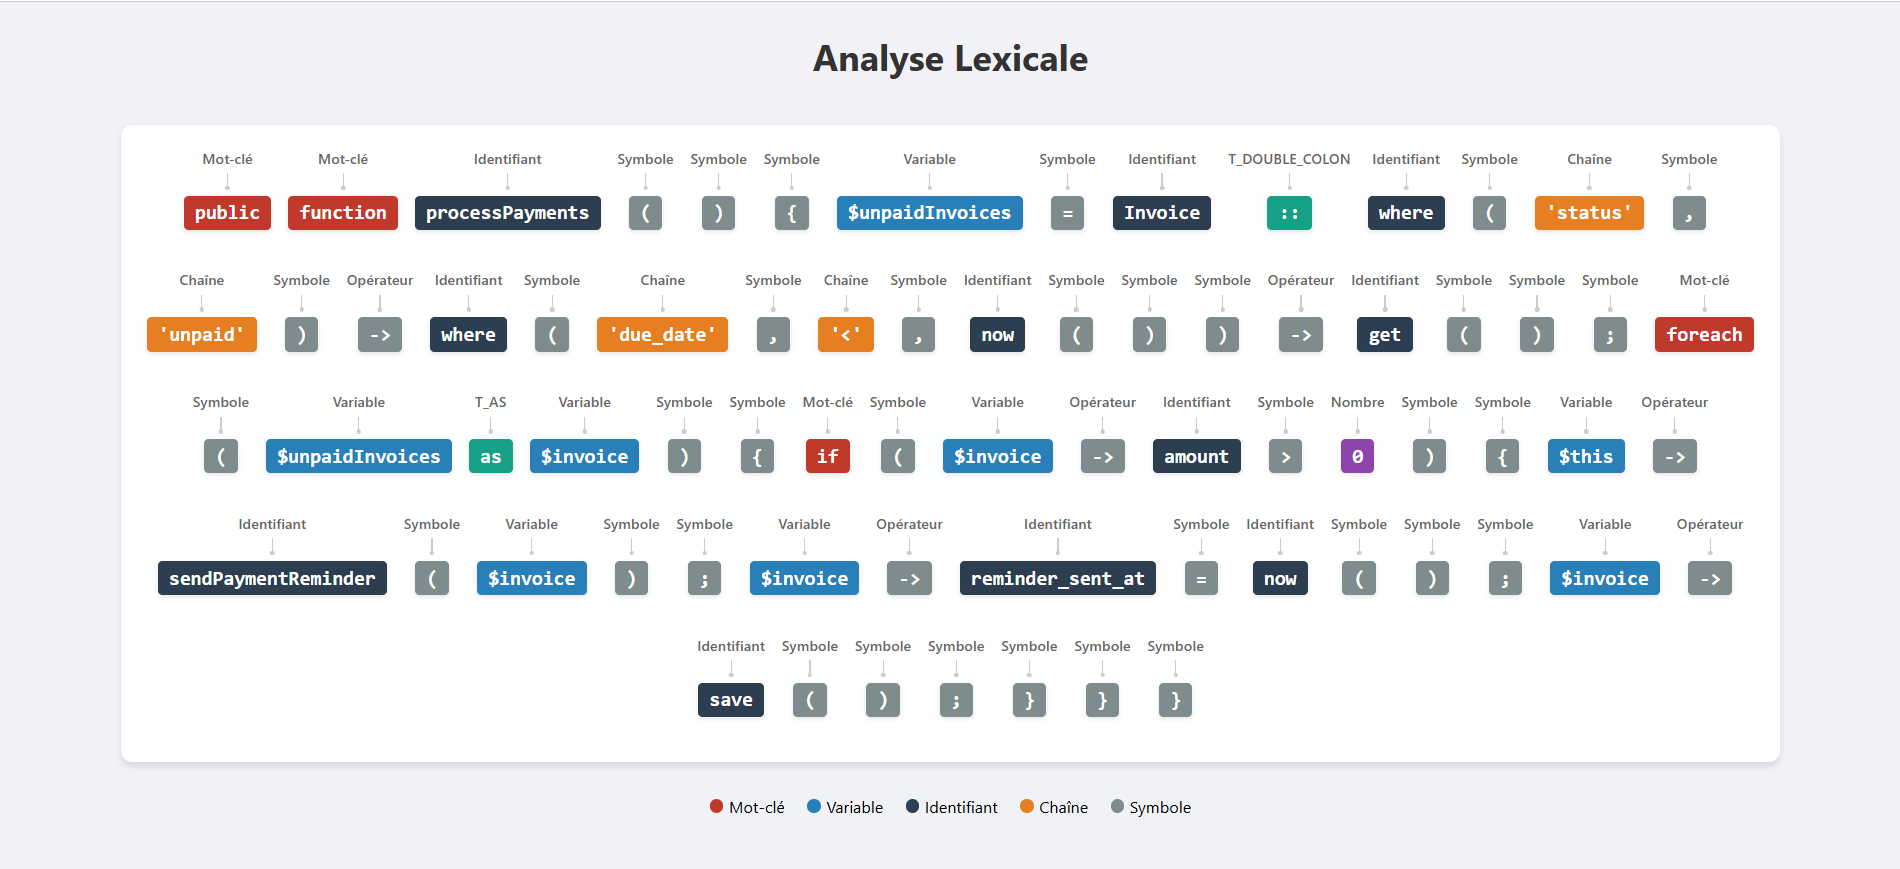
\includegraphics[width=0.7\textwidth]{analyse_lexical_code3.png}
    \caption{Analyse Lexicale - Code 3}
\end{figure}

\begin{figure}[H]
    \centering
    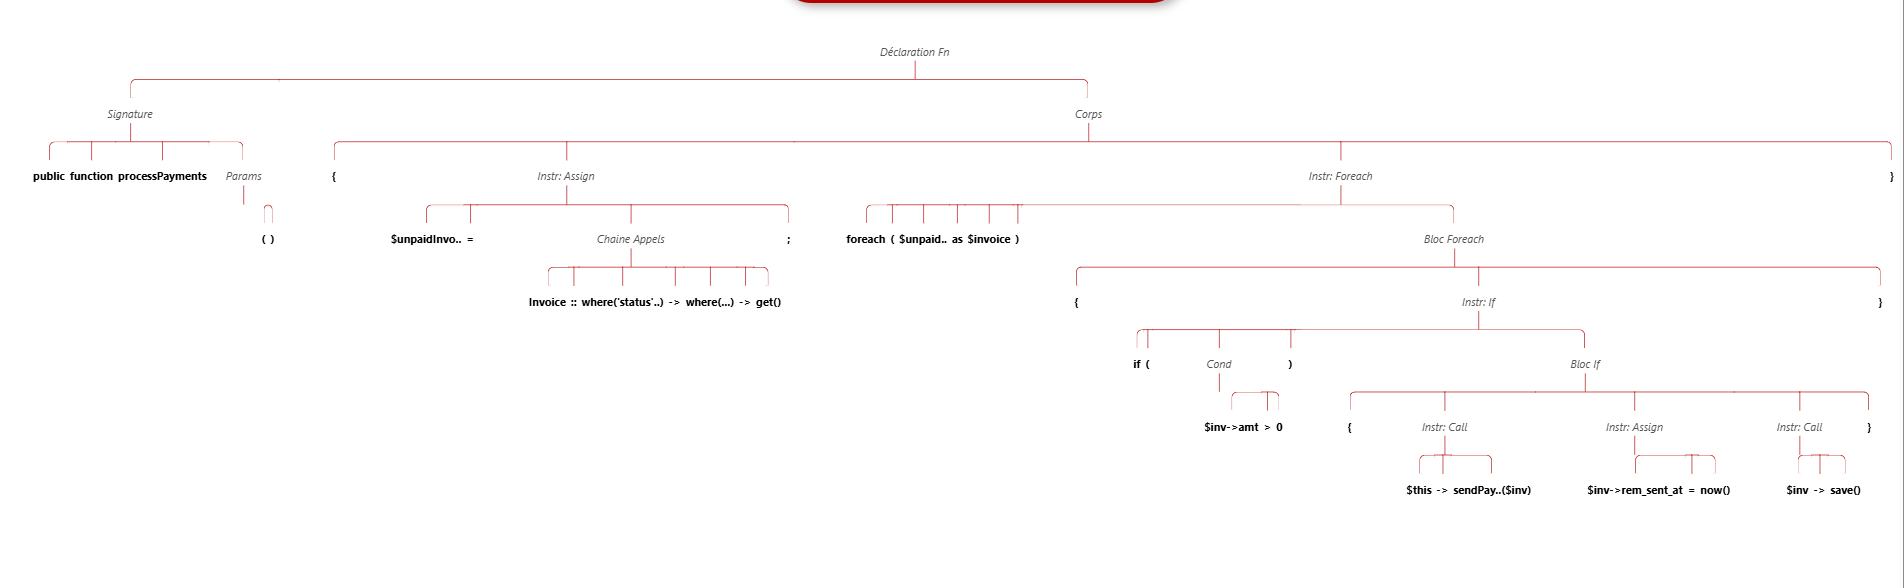
\includegraphics[width=0.8\textwidth]{analyse_syntaxique_code3.png}
    \caption{Analyse Syntaxique - Code 3}
\end{figure}

\begin{figure}[H]
    \centering
    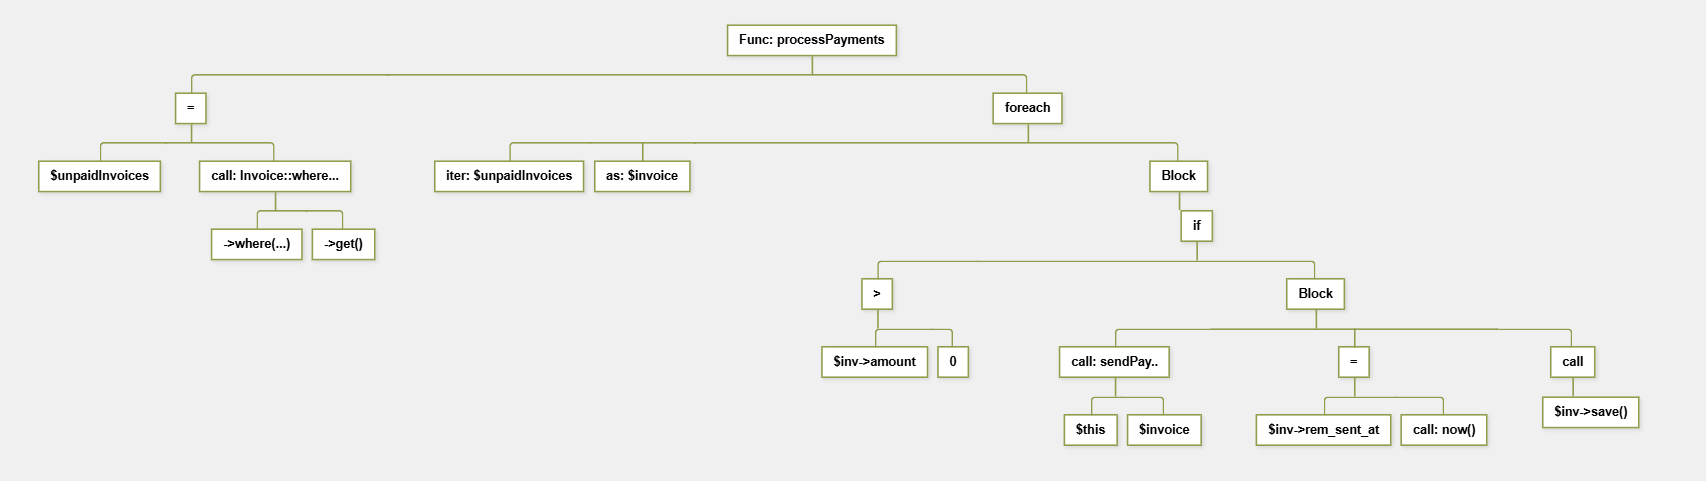
\includegraphics[width=0.8\textwidth]{analyse_sementique_code3.png}
    \caption{Analyse Sémantique - Code 3}
\end{figure}

\begin{figure}[H]
    \centering
    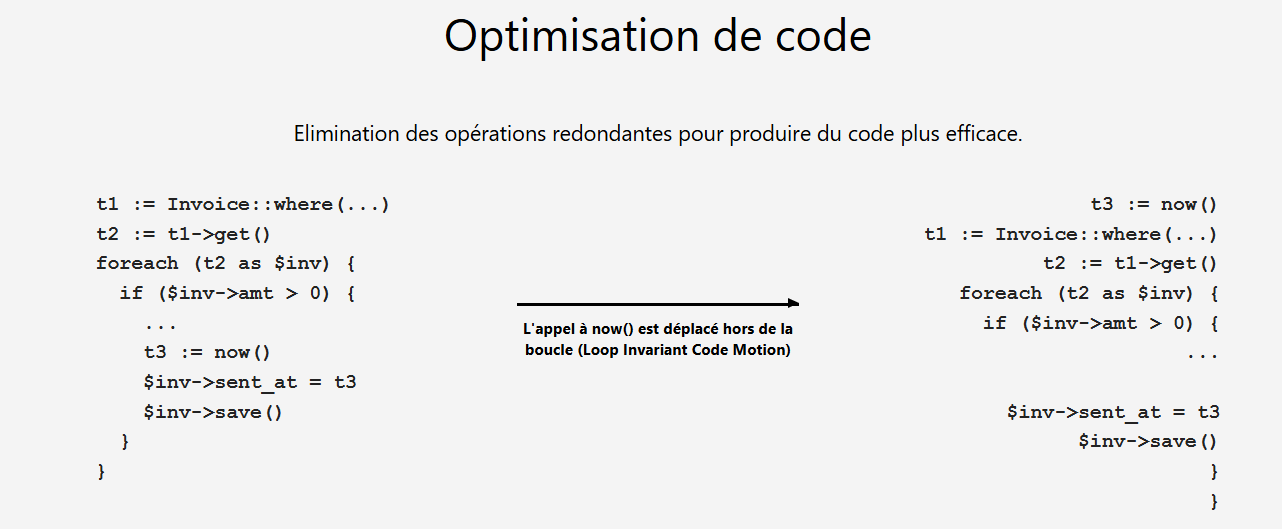
\includegraphics[width=0.8\textwidth]{optimisation_code3.png}
    \caption{Optimisation - Code 3}
\end{figure}

\begin{figure}[H]
    \centering
    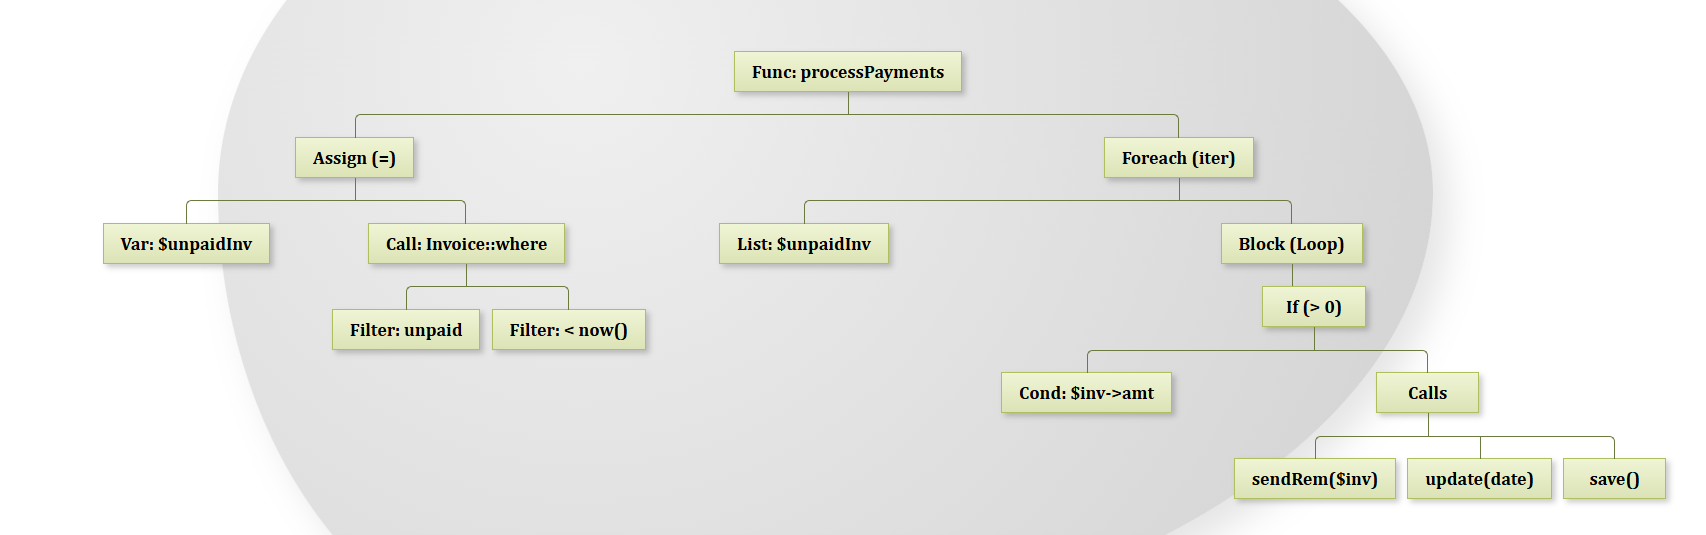
\includegraphics[width=0.8\textwidth]{generation_code3.png}
    \caption{Génération de Code - Code 3}
\end{figure}

\newpage
\section{Étude du Code 4 : Statistiques Dashboard}

Cette fonction illustre la logique conditionnelle complexe avec agrégations et calculs basés sur le rôle utilisateur.

\subsection{Analyse de la Fonction}

\begin{lstlisting}[style=phpstyle, caption=Fonction dashboardStats]
public function dashboardStats(Request $request)
{
    $user = $request->user();
    $data = [];
    if ($user->isAdmin()) {
        $data['totalUsers'] = User::count();
        $data['activeUsers'] = User::where('last_login', '>=', now()->subDays(30))->count();
    } else {
        $data['appointments'] = $user->appointments()->whereDate('appointment_date', '>=', now())->count();
        $data['unreadMessages'] = $user->unreadMessages()->count();
    }
    return response()->json($data);
}
\end{lstlisting}

\subsubsection{Description Fonctionnelle}

Cette fonction génère des statistiques personnalisées selon le rôle de l'utilisateur. Les administrateurs reçoivent des statistiques globales (total d'utilisateurs, utilisateurs actifs), tandis que les autres utilisateurs reçoivent leurs statistiques personnelles (rendez-vous à venir, messages non lus).

\subsubsection{Points Techniques}

\begin{itemize}
    \item Récupération de l'utilisateur depuis la requête
    \item Logique conditionnelle basée sur le rôle (\texttt{isAdmin()})
    \item Agrégations avec \texttt{count()} sur différentes relations
    \item Calcul de dates avec \texttt{now()->subDays(30)}
    \item Utilisation de relations Eloquent (\texttt{appointments()}, \texttt{unreadMessages()})
    \item Pattern de réponse différenciée selon le contexte
\end{itemize}

\begin{figure}[H]
    \centering
    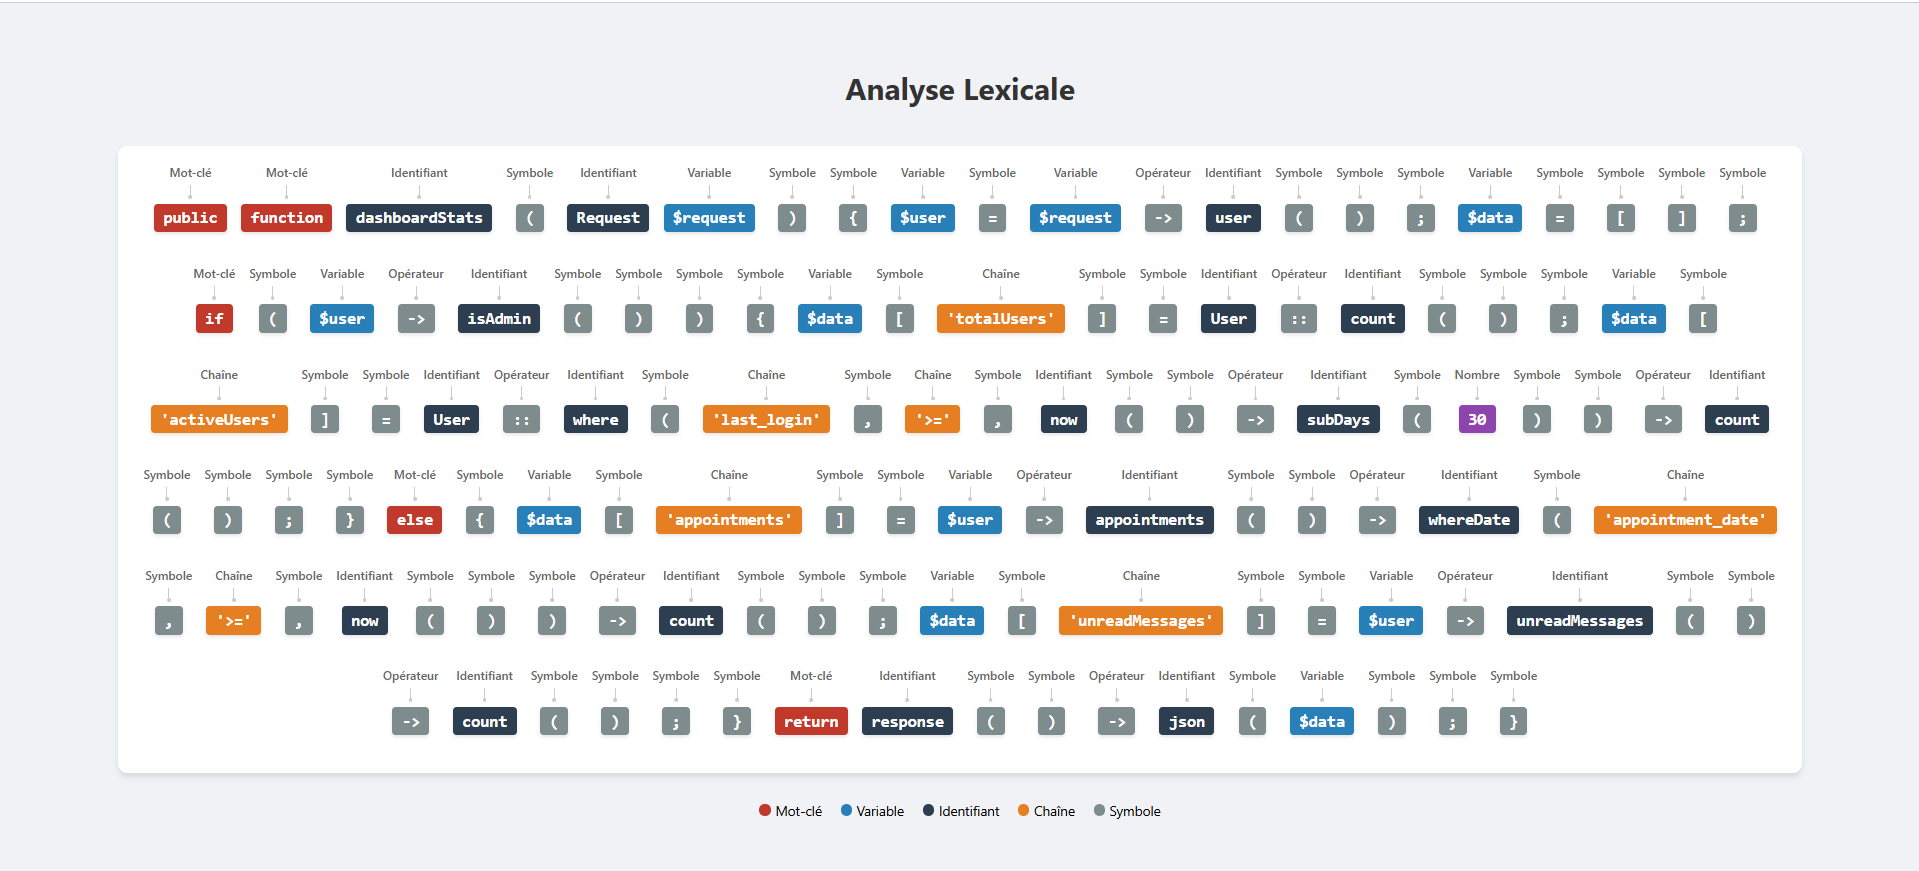
\includegraphics[width=0.7\textwidth]{analyse_lexical_code4.png}
    \caption{Analyse Lexicale - Code 4}
\end{figure}

\begin{figure}[H]
    \centering
    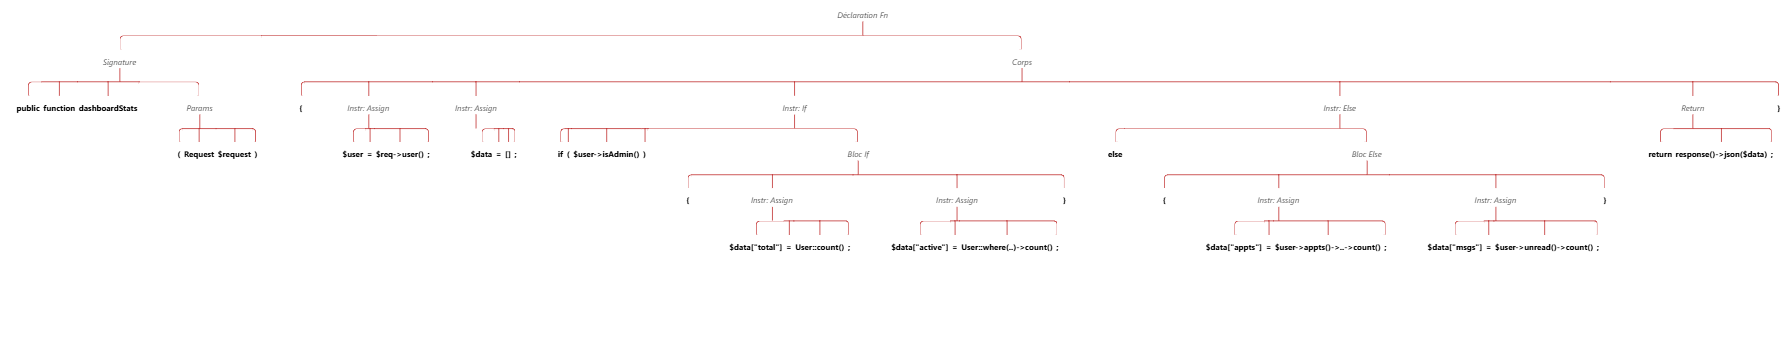
\includegraphics[width=0.8\textwidth]{analyse_syntaxique_code4.png}
    \caption{Analyse Syntaxique - Code 4}
\end{figure}

\begin{figure}[H]
    \centering
    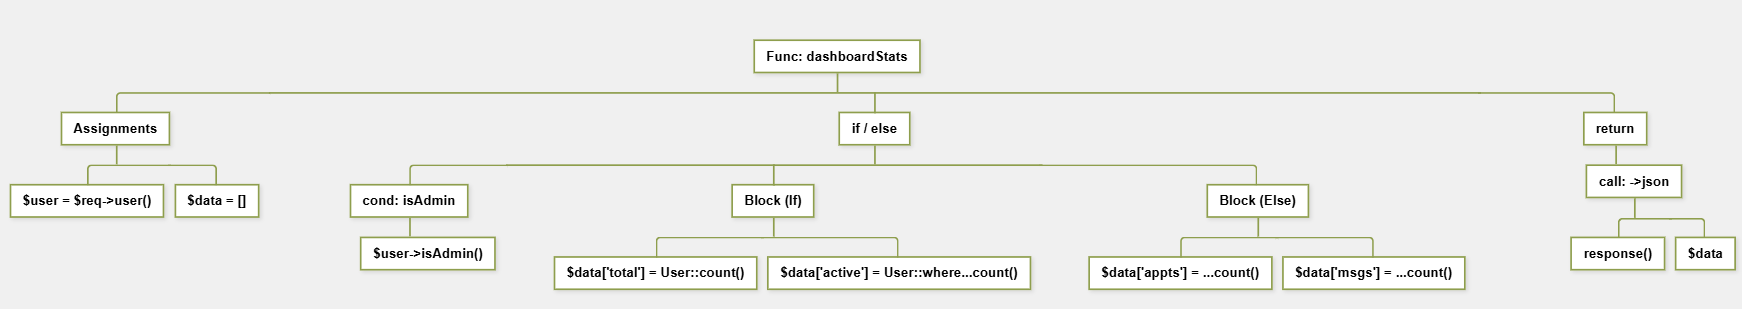
\includegraphics[width=0.8\textwidth]{analyse_sementique_code4.png}
    \caption{Analyse Sémantique - Code 4}
\end{figure}

\begin{figure}[H]
    \centering
    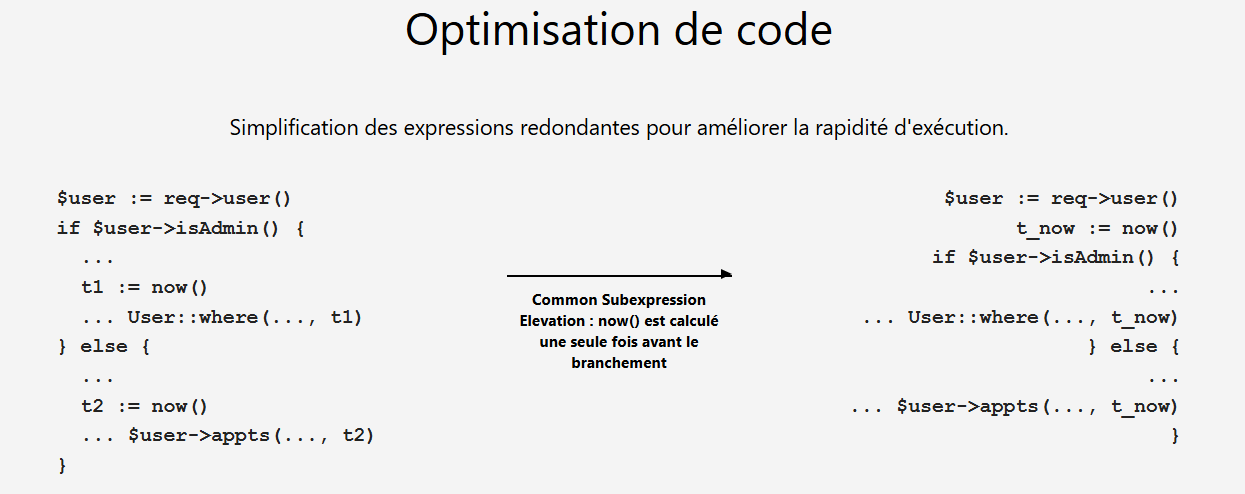
\includegraphics[width=0.8\textwidth]{optimisation_code4.png}
    \caption{Optimisation - Code 4}
\end{figure}

\begin{figure}[H]
    \centering
    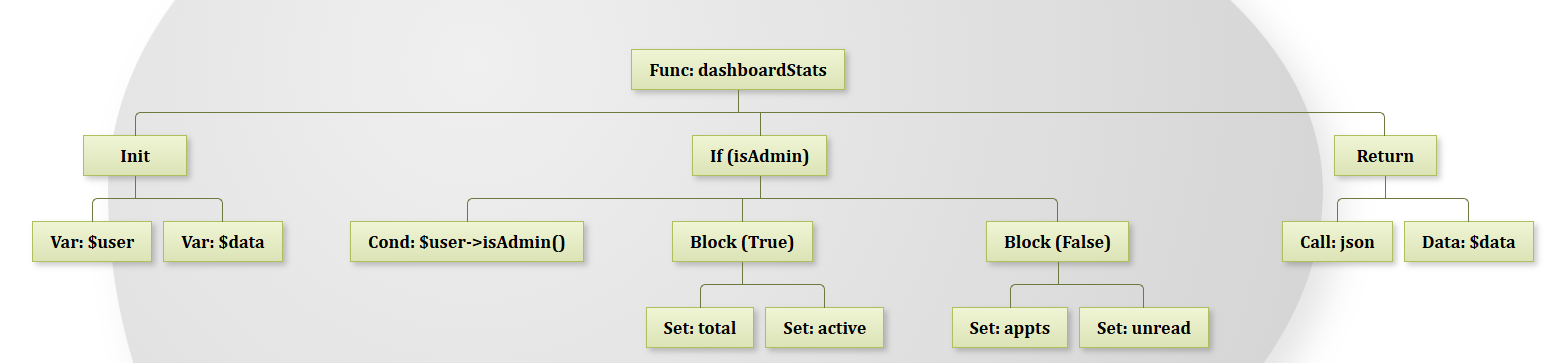
\includegraphics[width=0.8\textwidth]{generation_code4.png}
    \caption{Génération de Code - Code 4}
\end{figure}

\newpage
\section{Étude du Code 5 : Enregistrement d'une tâche}

Cette fonction illustre la gestion de fichiers, la validation de formulaires et la création de ressources avec données optionnelles.

\subsection{Analyse de la Fonction}

\begin{lstlisting}[style=phpstyle, caption=Fonction store]
public function store(Request $request)
{
    $validated = $request->validate([
        'title' => 'required|string|max:100',
        'due_date' => 'required|date|after:today'
    ]);
    $task = new Task($validated);
    if ($request->hasFile('attachment')) {
        $path = $request->file('attachment')->store('attachments');
        $task->attachment_path = $path;
    }
    $task->save();
    return response()->json($task, 201);
}
\end{lstlisting}

\subsubsection{Description Fonctionnelle}

Cette fonction crée une nouvelle tâche avec validation des données et gestion optionnelle d'un fichier joint. Elle utilise la validation intégrée de Laravel directement sur la requête, puis crée le modèle avec les données validées. Si un fichier est présent, il est stocké et son chemin est enregistré.

\subsubsection{Points Techniques}

\begin{itemize}
    \item Validation directe sur \texttt{\$request} avec \texttt{validate()}
    \item Règle de validation temporelle \texttt{after:today}
    \item Création de modèle avec données validées via constructeur
    \item Gestion conditionnelle de fichiers avec \texttt{hasFile()}
    \item Stockage de fichiers avec \texttt{store()} dans un dossier dédié
    \item Code HTTP 201 (Created) pour création réussie
    \item Pattern de création de ressource RESTful complet
\end{itemize}

\begin{figure}[H]
    \centering
    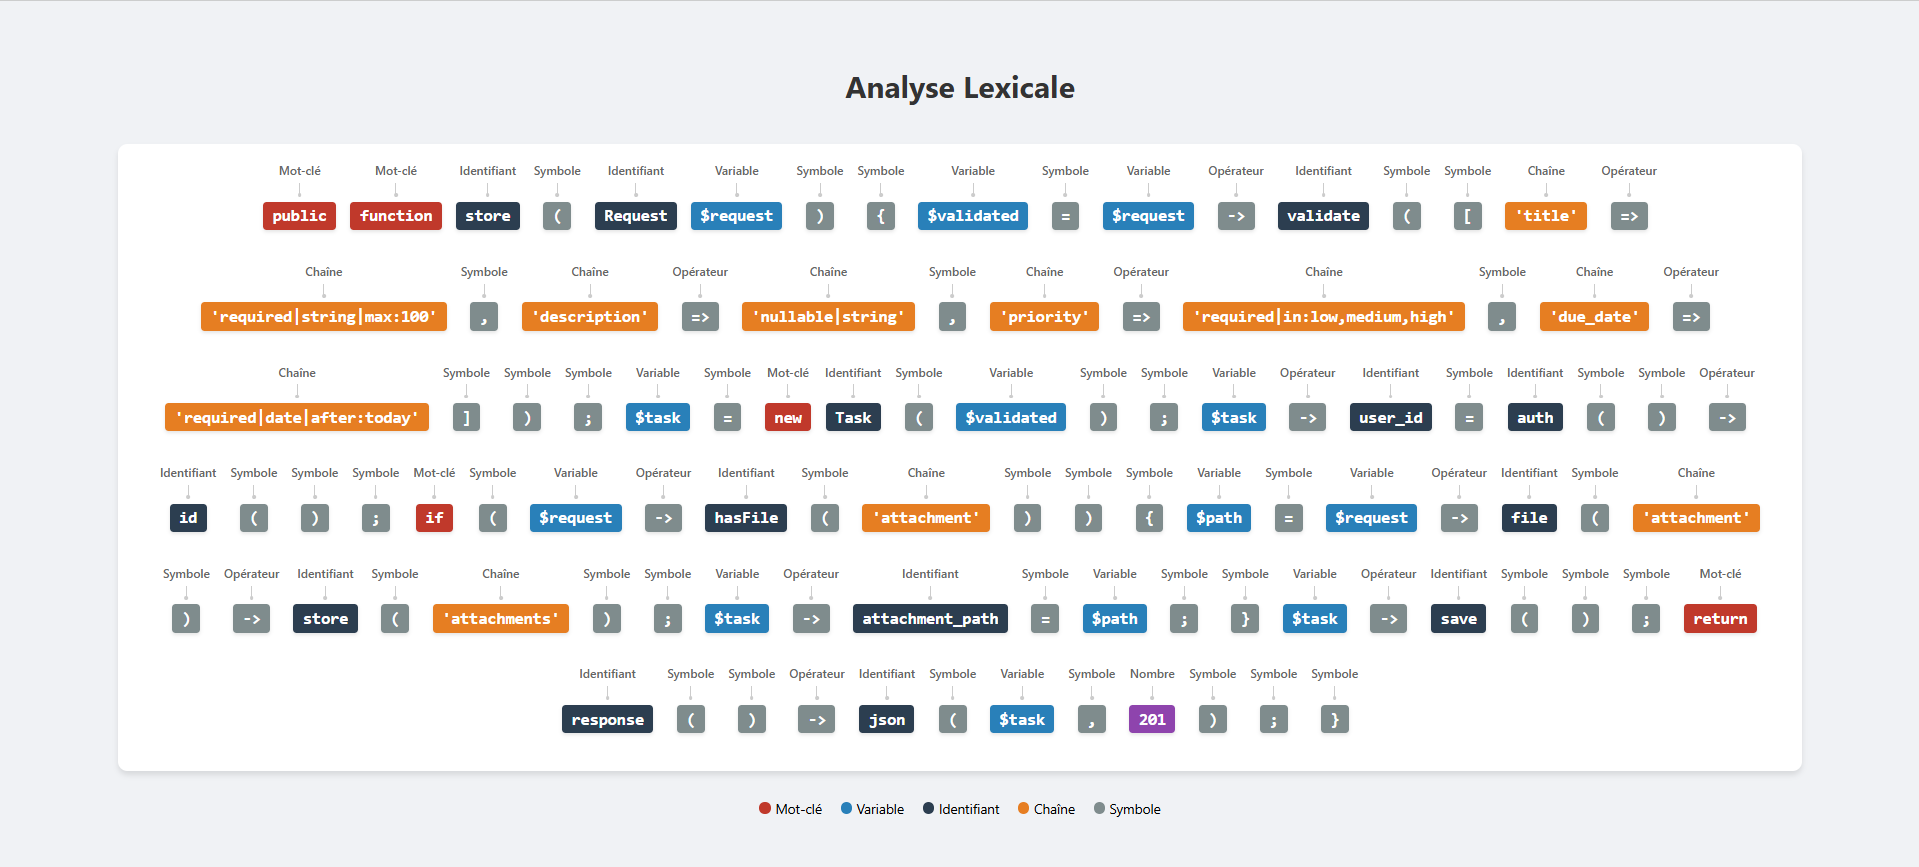
\includegraphics[width=0.7\textwidth]{analyse_lexical_code5.png}
    \caption{Analyse Lexicale - Code 5}
\end{figure}

\begin{figure}[H]
    \centering
    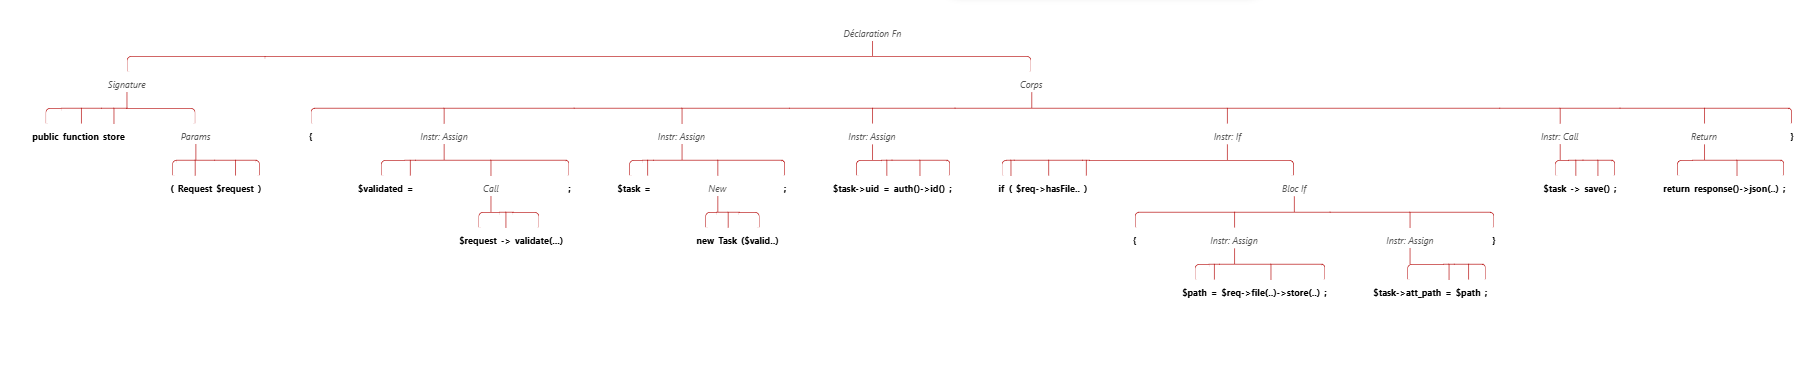
\includegraphics[width=0.8\textwidth]{analyse_syntaxique_code5.png}
    \caption{Analyse Syntaxique - Code 5}
\end{figure}

\begin{figure}[H]
    \centering
    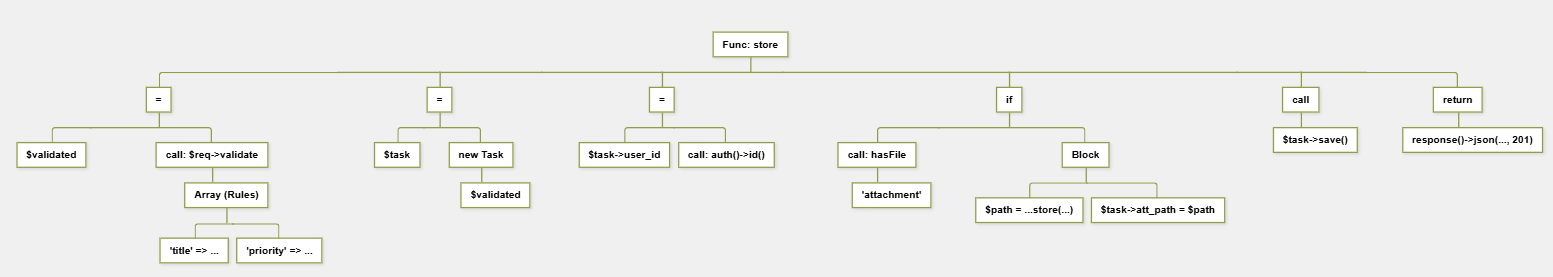
\includegraphics[width=0.8\textwidth]{analyse_sementique_code5.png}
    \caption{Analyse Sémantique - Code 5}
\end{figure}

\begin{figure}[H]
    \centering
    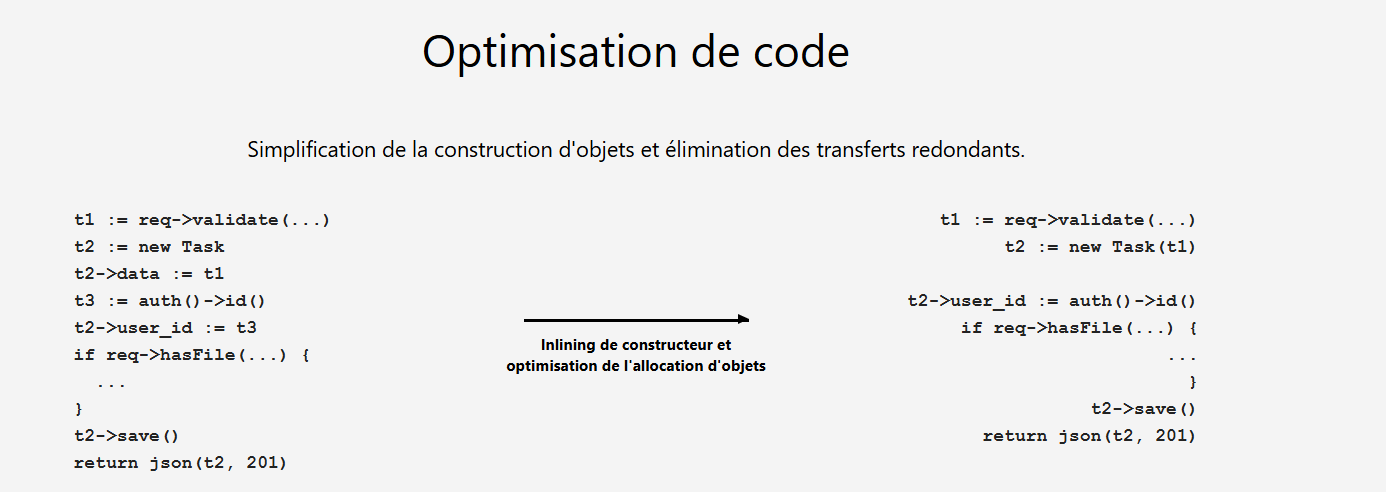
\includegraphics[width=0.8\textwidth]{optimisation_code5.png}
    \caption{Optimisation - Code 5}
\end{figure}

\begin{figure}[H]
    \centering
    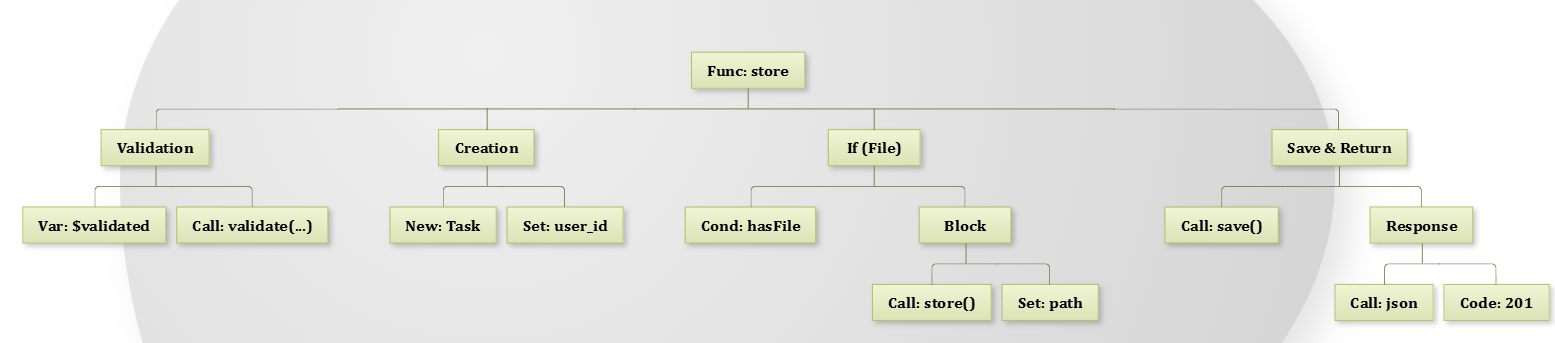
\includegraphics[width=0.8\textwidth]{generation_code5.png}
    \caption{Génération de Code - Code 5}
\end{figure}

\chapter{Conclusion Générale}

\section{Résumé du Projet}

Ce rapport a présenté l'analyse, la conception et la réalisation complète d'un système de gestion de cabinet dentaire, ainsi qu'une exploration approfondie des phases de compilation. Les éléments principaux développés sont :

\begin{itemize}
    \item \textbf{Analyse des besoins} : Identification complète des acteurs (Patient, Docteur, Personnel Administratif, Système de Notifications), fonctionnalités détaillées et contraintes techniques et fonctionnelles du système.
    \item \textbf{Modélisation UML} : Conception structurée à travers trois diagrammes essentiels :
    \begin{itemize}
        \item Diagramme de cas d'utilisation avec relations \texttt{includes} et \texttt{extends}
        \item Diagramme de séquence illustrant les interactions temporelles
        \item Diagramme de classes avec hiérarchie d'héritage et relations d'association
    \end{itemize}
    \item \textbf{Base de données} : Schéma relationnel normalisé (3NF) avec 11 tables principales, 3 vues optimisées, index stratégiques et contraintes d'intégrité référentielle sous MySQL.
    \item \textbf{Réalisation logicielle} : Implémentation complète d'une application web moderne :
    \begin{itemize}
        \item Frontend React avec TypeScript, Tailwind CSS et architecture modulaire
        \item Backend Laravel 12 avec API RESTful complète (8 contrôleurs, 8 modèles)
        \item Authentification JWT sécurisée avec gestion des rôles
        \item 15+ composants React réutilisables et services API organisés
    \end{itemize}
    \item \textbf{Module de compilation} : Démonstration détaillée des cinq phases de compilation (lexicale, syntaxique, sémantique, optimisation, génération) appliquées à cinq fonctions critiques du système.
\end{itemize}

\section{Bilan Technique et Apports}

\subsection{Maîtrise Technique Acquise}

La réalisation de ce projet a permis d'acquérir une expertise approfondie dans plusieurs domaines :

\textbf{Architecture et Conception :}
\begin{itemize}
    \item Maîtrise de l'architecture découplée (frontend/backend)
    \item Conception d'API RESTful selon les standards
    \item Modélisation UML complète (cas d'utilisation, séquence, classes)
    \item Normalisation de base de données (3NF) avec optimisation des requêtes
\end{itemize}

\textbf{Développement Frontend :}
\begin{itemize}
    \item Maîtrise de React 18 avec hooks et gestion d'état
    \item Utilisation de TypeScript pour la robustesse du code
    \item Design responsive avec Tailwind CSS
    \item Gestion des appels API avec Axios et intercepteurs
    \item Architecture modulaire avec séparation des responsabilités
\end{itemize}

\textbf{Développement Backend :}
\begin{itemize}
    \item Maîtrise de Laravel 12 avec Eloquent ORM
    \item Implémentation d'authentification JWT sécurisée
    \item Validation de données avec règles personnalisées
    \item Gestion des relations complexes entre modèles
    \item Optimisation des requêtes (eager loading, index)
\end{itemize}

\textbf{Sécurité et Bonnes Pratiques :}
\begin{itemize}
    \item Hachage sécurisé des mots de passe (BCrypt)
    \item Protection contre les injections SQL (via Eloquent)
    \item Gestion fine des permissions selon les rôles
    \item Validation stricte des données d'entrée
    \item Gestion des erreurs et codes HTTP appropriés
\end{itemize}

\subsection{Apports du Module de Compilation}

L'étude du module de compilation a permis de :
\begin{itemize}
    \item Comprendre les mécanismes internes des langages de programmation
    \item Analyser le processus de transformation du code source
    \item Identifier les optimisations possibles dans le code
    \item Appréhender la complexité des compilateurs et interpréteurs
    \item Appliquer ces connaissances à l'optimisation de notre propre code
\end{itemize}

\subsection{Enjeux Métier Compris}

Ce projet a également permis de comprendre les enjeux spécifiques au domaine médical :
\begin{itemize}
    \item Confidentialité et protection des données médicales sensibles
    \item Conformité aux réglementations sur la protection des données
    \item Gestion des contraintes temporelles (rendez-vous, rappels)
    \item Traçabilité des actions (historique des traitements)
    \item Interface intuitive pour différents profils d'utilisateurs
\end{itemize}

\section{Perspectives d'Évolution}

Cette base solide et bien architecturée permet d'envisager plusieurs évolutions futures :

\subsection{Évolutions Fonctionnelles}

\begin{itemize}
    \item \textbf{Module de Paiement} : Intégration d'une passerelle de paiement en ligne pour les traitements médicaux (Stripe, PayPal)
    \item \textbf{Application Mobile} : Développement d'une application mobile native (React Native ou Flutter) pour les patients
    \item \textbf{Télémédecine} : Intégration de visioconférence pour consultations à distance
    \item \textbf{Gestion Multi-Cabinets} : Extension du système pour gérer plusieurs cabinets avec centralisation des données
    \item \textbf{Rapports Avancés} : Génération de rapports PDF/Excel avec statistiques détaillées et graphiques
\end{itemize}

\subsection{Évolutions Techniques}

\begin{itemize}
    \item \textbf{Intelligence Artificielle} : Utilisation de l'IA pour l'aide au diagnostic à partir des dossiers médicaux
    \item \textbf{Real-time} : Intégration de WebSockets pour les notifications en temps réel
    \item \textbf{Cache} : Mise en place de Redis pour le cache des requêtes fréquentes
    \item \textbf{Search} : Intégration d'Elasticsearch pour la recherche avancée dans les dossiers
    \item \textbf{Microservices} : Migration vers une architecture microservices pour une meilleure scalabilité
\end{itemize}

\subsection{Améliorations Continues}

\begin{itemize}
    \item Tests automatisés complets (unitaires, intégration, end-to-end)
    \item CI/CD avec déploiement automatique
    \item Monitoring et logging avancés (Sentry, LogRocket)
    \item Documentation API complète (Swagger/OpenAPI)
    \item Optimisation continue des performances
\end{itemize}

\section{Conclusion}

Ce projet constitue une démonstration complète de maîtrise du cycle de développement logiciel, de l'analyse des besoins à la réalisation technique, en passant par la modélisation UML et la conception de base de données. 

L'application développée répond aux exigences fonctionnelles et non fonctionnelles définies, avec une architecture moderne, sécurisée et évolutive. Le module d'analyse de compilation ajoute une dimension pédagogique importante, permettant de comprendre les mécanismes internes des langages de programmation.

Ce travail démontre :
\begin{itemize}
    \item Une capacité d'analyse et de conception rigoureuse
    \item Une maîtrise technique des technologies modernes (React, Laravel, TypeScript)
    \item Une compréhension approfondie des enjeux de sécurité et de performance
    \item Une approche méthodique et professionnelle du développement logiciel
    \item Une capacité à documenter et présenter un projet complexe
\end{itemize}

En conclusion, ce système de gestion de cabinet dentaire représente une solution professionnelle, complète et évolutive, prête à être déployée dans un environnement de production, tout en conservant la flexibilité nécessaire pour s'adapter aux besoins futurs.


\end{document}